% Chapter 6: State space models and Bayesian filtering
% Advanced Time Series Analysis and Forecasting -- Master's programme Applied Statistics and Data Science, year 1, semester 2, Bucharest University of Economic Studies
% GENERATED by latex/build_chapter6.py -- edit the generator, not this file.

\newcommand{\coursename}{Advanced Time Series Analysis and Forecasting}
% Preambul comun ATS -- Analiza avansată a seriilor de timp și previziune / Advanced Time Series Analysis and Forecasting
% (Beamer, 16:9). Același design ca MFM, SFM și TSA (copiat din TSA, 5 octombrie 2026). Înainte de % Preambul comun ATS -- Analiza avansată a seriilor de timp și previziune / Advanced Time Series Analysis and Forecasting
% (Beamer, 16:9). Același design ca MFM, SFM și TSA (copiat din TSA, 5 octombrie 2026). Înainte de % Preambul comun ATS -- Analiza avansată a seriilor de timp și previziune / Advanced Time Series Analysis and Forecasting
% (Beamer, 16:9). Același design ca MFM, SFM și TSA (copiat din TSA, 5 octombrie 2026). Înainte de \input{../../latex/preamble} se definește
%   \newcommand{\coursename}{Advanced Time Series Analysis and Forecasting}          (EN)
%   \newcommand{\coursename}{Analiza avansată a seriilor de timp și previziune}       (RO)  și  \def\atslang{ro}
% Fișierele .tex se află în EN/Courses, EN/Seminars, RO/Cursuri, RO/Seminarii (două niveluri sub rădăcină).
% Deck-urile sînt generate de latex/build_chapterN.py / build_seminarN.py (vezi latex/ats_build.py).

\documentclass[9pt, aspectratio=169, t]{beamer}
\providecommand{\coursename}{Advanced Time Series Analysis and Forecasting}

% Ensure content fits on slides
\setbeamersize{text margin left=8mm, text margin right=8mm}
% Smaller institute font (title page)
\setbeamerfont{institute}{size=\footnotesize}

%=============================================================================
% THEME AND STYLE CONFIGURATION
%=============================================================================
\usetheme{default}
% Using default theme for clean header/footer control

% Color Palette (matching Redispatch PDF)
\definecolor{MainBlue}{RGB}{26, 58, 110}
\definecolor{AccentBlue}{RGB}{26, 58, 110}
\definecolor{IDAred}{RGB}{205, 0, 0}
\definecolor{DarkGray}{RGB}{51, 51, 51}
\definecolor{MediumGray}{RGB}{128, 128, 128}
\definecolor{LightGray}{RGB}{248, 248, 248}
\definecolor{VeryLightGray}{RGB}{235, 235, 235}
\definecolor{KeynoteGray}{RGB}{218, 218, 218}
\definecolor{SectionGray}{RGB}{120, 120, 120}
\definecolor{FooterGray}{RGB}{100, 100, 100}
\definecolor{Crimson}{RGB}{220, 53, 69}
\definecolor{Forest}{RGB}{46, 125, 50}
\definecolor{Amber}{RGB}{181, 133, 63}
\definecolor{Orange}{RGB}{230, 126, 34}
\definecolor{Purple}{RGB}{142, 68, 173}

% Gradient background (exact Keynote 315° gradient: white to RGB 218,218,218)
\setbeamertemplate{background}{%
    \begin{tikzpicture}[remember picture, overlay]
        \shade[shading=axis, shading angle=315,
        top color=white, bottom color=KeynoteGray]
        (current page.south west) rectangle (current page.north east);
    \end{tikzpicture}%
}
% Fallback solid color for compatibility
\setbeamercolor{background canvas}{bg=}

\setbeamercolor{palette primary}{bg=MainBlue, fg=white}
\setbeamercolor{palette secondary}{bg=MainBlue!85, fg=white}
\setbeamercolor{palette tertiary}{bg=MainBlue!70, fg=white}
\setbeamercolor{structure}{fg=MainBlue}
\setbeamercolor{title}{fg=IDAred}
\setbeamercolor{frametitle}{fg=IDAred, bg=}
\setbeamercolor{block title}{bg=MainBlue, fg=white}
\setbeamercolor{block body}{bg=VeryLightGray, fg=DarkGray}
\setbeamercolor{block title alerted}{bg=Crimson, fg=white}
\setbeamercolor{block body alerted}{bg=Crimson!8, fg=DarkGray}
\setbeamercolor{block title example}{bg=Forest, fg=white}
\setbeamercolor{block body example}{bg=Forest!8, fg=DarkGray}
\setbeamercolor{item}{fg=MainBlue}

% Footer colors (override Madrid theme blue)
\setbeamercolor{author in head/foot}{fg=FooterGray, bg=}
\setbeamercolor{title in head/foot}{fg=FooterGray, bg=}
\setbeamercolor{date in head/foot}{fg=FooterGray, bg=}
\setbeamercolor{section in head/foot}{fg=FooterGray, bg=}
\setbeamercolor{subsection in head/foot}{fg=FooterGray, bg=}

% Bullet styles (apply everywhere including blocks)
\setbeamertemplate{itemize item}{\color{MainBlue}$\boxdot$}
\setbeamertemplate{itemize subitem}{\color{MainBlue}$\blacktriangleright$}
\setbeamertemplate{itemize subsubitem}{\color{MainBlue}\tiny$\bullet$}
\setbeamertemplate{itemize/enumerate body begin}{\normalsize}
\setbeamertemplate{itemize/enumerate subbody begin}{\normalsize}

% Item spacing - compact style
\setlength{\leftmargini}{10pt}       % Level 1: minimal indent
\setlength{\leftmarginii}{10pt}      % Level 2: minimal additional indent
% Compact list spacing (zero extra space before/after lists in blocks)
\makeatletter
\def\@listi{\leftmargin\leftmargini \topsep 0pt \parsep 0pt \itemsep 0pt}
\def\@listii{\leftmargin\leftmarginii \topsep 0pt \parsep 0pt \itemsep 0pt}
\makeatother

\setbeamertemplate{navigation symbols}{}

%=============================================================================
% CUSTOM HEADLINE
%=============================================================================
\setbeamertemplate{headline}{%
    \vskip10pt%
    \hbox to \paperwidth{%
        \hskip0.5cm%
        {\small\color{FooterGray}\renewcommand{\hyperlink}[2]{##2}\insertsectionhead}%
        \hfill%
        \textcolor{FooterGray}{\small\insertframenumber}%
        \hskip0.5cm%
    }%
    \vskip4pt%
    {\color{FooterGray}\hrule height 0.4pt}%
}

%=============================================================================
% CUSTOM FOOTER
%=============================================================================
\usepackage{fontawesome5}

\setbeamertemplate{footline}{%
    {\color{FooterGray}\hrule height 0.4pt}%
    \vskip4pt%
    \hbox to \paperwidth{%
        \hskip0.5cm%
        \textcolor{FooterGray}{\small\coursename}%
        \hfill%
        \raisebox{-0.1em}{%
            \begin{tikzpicture}[x=0.08em, y=0.08em, line width=0.4pt]
                \draw[FooterGray] (0,3) -- (1,4) -- (2,3.5) -- (3,5) -- (4,4) -- (5,6) -- (6,5.5) -- (7,4) -- (8,5) -- (9,7) -- (10,6) -- (11,5) -- (12,6.5) -- (13,8) -- (14,7) -- (15,6) -- (16,7.5) -- (17,9) -- (18,8) -- (19,7) -- (20,8.5) -- (21,10) -- (22,9) -- (23,8) -- (24,9.5);
            \end{tikzpicture}%
        }%
        \hskip0.5cm%
    }%
    \vskip6pt%
}

%=============================================================================
% PACKAGES
%=============================================================================
\usepackage[utf8]{inputenc}
\DeclareUnicodeCharacter{03B1}{\ensuremath{\alpha}}
\usepackage[T1]{fontenc}
\usepackage{amsmath, amssymb, amsthm}
\usepackage{mathtools}
\usepackage{bm}
\usepackage{tikz}
\usetikzlibrary{arrows.meta, positioning, shapes, calc, decorations.pathreplacing, shadings}
\usepackage{booktabs}
\usepackage{multirow}
\usepackage{array}
\usepackage{graphicx}
\usepackage{animate}
\usepackage{hyperref}
\usepackage{colortbl}
\usepackage{listings}
\lstset{language=Python, basicstyle=\ttfamily\scriptsize, keywordstyle=\color{MainBlue}\bfseries,
  commentstyle=\color{Forest}, stringstyle=\color{Crimson}, breaklines=true,
  frame=none, backgroundcolor=\color{VeryLightGray}, xleftmargin=2mm}
\hypersetup{colorlinks=true, linkcolor=MainBlue, urlcolor=MainBlue}
\graphicspath{{../../logos/}{../../charts/}{../../photos/}}
\usepackage{xcolor}
\hfuzz=2pt  % Suppress tiny overfull warnings (<2pt)
\vfuzz=2pt  % Suppress tiny vertical overfull warnings (<2pt)

%=============================================================================
% QUANTLET COMMANDS
%   \quantlet{<displayed name>}{<url>}       (generic)
%   \atsquantlet{Ch_05}{ATS_ch5_garch}       -> https://github.com/danpele/Advanced-Time-Series/tree/main/Quantlets/Ch_05/ATS_ch5_garch
%   \qlurl{<folder>} is defined per chapter by the generator (Quantlets/Ch_NN/<folder>)
%=============================================================================
\newcommand{\atsrepo}{https://github.com/danpele/Advanced-Time-Series}
\newcommand{\atsqlbase}{https://github.com/danpele/Advanced-Time-Series/tree/main/Quantlets}
\newcommand{\quantlet}[2]{%
    \hfill\href{#2}{%
        \raisebox{-0.15em}{
\includegraphics[height=0.7em]{ql_logo.png}}%
        \textcolor{MainBlue}{\tiny\ #1}%
    }%
}
\newcommand{\atsquantlet}[2]{\quantlet{\detokenize{#2}}{\atsqlbase/#1/#2}}

%=============================================================================
% NOTEBOOKS (Google Colab)
%   \colaburl{notebooks/EN/chapter5_seminar_notebook.ipynb} -> the Colab link of a file in the ATS repo
%   \nb: the chapter notebook (each seminar deck redefines it with \renewcommand)
%=============================================================================
\newcommand{\colaburl}[1]{https://colab.research.google.com/github/danpele/Advanced-Time-Series/blob/main/#1}
\newcommand{\nb}{https://colab.research.google.com/github/danpele/Advanced-Time-Series/tree/main/notebooks/EN}
\newcommand{\nbname}{notebooks/EN}

%=============================================================================
% SLIDE HELPERS (used by the generators; the same as in MFM)
%=============================================================================
% local font size for list bodies (the preamble forces \normalsize)
\newcommand{\itemsize}[1]{\setbeamertemplate{itemize/enumerate body begin}{#1}\setbeamertemplate{itemize/enumerate subbody begin}{#1}}
\newcommand{\intitle}[1]{{\hypersetup{urlcolor=white}#1}}   % white links inside coloured title bars
\newcommand{\imgcap}[1]{{\scriptsize #1}\\[0.5mm]}          % caption under a photo
\newcommand{\imgcredit}[2]{{\tiny\color{FooterGray}\href{#1}{#2}}}   % image credit: source URL, author/licence
\newcommand{\aiprompt}[1]{{\ttfamily\color{MainBlue}#1}}     % a prompt to an AI assistant

%=============================================================================
% SEMINARS: student version by default; the instructor wrapper *_solutions.tex sets \solutionstrue
%=============================================================================
\makeatletter\@ifundefined{ifsolutions}{\expandafter\newif\csname ifsolutions\endcsname}{}\makeatother
\newcommand{\solonly}[1]{\ifsolutions #1\fi}
\newcommand{\propsub}{\ifsolutions\else\framesubtitle{\ifdefined\atslang Rezolvarea se discută la seminar\else Solution discussed in class\fi}\fi}

%=============================================================================
% APPENDIX AND CHAPTER LINKS (latex/appendix_links.py writes the calls; it also re-declares these
% macros before \begin{document}, so the decks compile with or without this preamble block)
%=============================================================================
\providecommand{\atsapplink}[3]{\hypertarget{#2}{}\hyperlink{#1}{\beamergotobutton{#3}}}
\providecommand{\atsappback}[2]{\begin{tikzpicture}[remember picture,overlay]\node[anchor=south east] at ([xshift=-3mm,yshift=7mm]current page.south east){\hyperlink{#1}{\beamerreturnbutton{#2}}};\end{tikzpicture}}
\providecommand{\atschlink}[2]{\href{#1}{#2}}
\providecommand{\atschlinkt}[2]{\href{#1}{\usebeamercolor[fg]{frametitle}#2}}

%=============================================================================
% QUANTINAR COMMAND: link către un curs Quantinar (subiecte avansate)
%=============================================================================
\newcommand{\quantinar}[2]{%
    \href{#2}{%
        \raisebox{-0.15em}{
\includegraphics[height=0.8em]{qr_logo.png}}%
        \textcolor{MainBlue}{\scriptsize\ #1}%
    }%
}

%=============================================================================
% CUSTOM TITLE PAGE
%=============================================================================
\defbeamertemplate*{title page}{hybrid}[1][]
{
    \vspace{0.2cm}
    % Logos row - top header (with clickable links)
    \begin{center}
        \href{https://www.ase.ro}{
\includegraphics[height=1.0cm]{ase_logo.png}}\hspace{0.3cm}%
        \href{https://theida.net}{
\includegraphics[height=1.0cm]{ida_logo.png}}\hspace{0.3cm}%
        \href{https://blockchain-research-center.com}{
\includegraphics[height=1.0cm]{brc_logo.png}}\hspace{0.3cm}%
        \href{https://www.ai4efin.ase.ro}{
\includegraphics[height=1.0cm]{ai4efin_logo.png}}\hspace{0.3cm}%
        \href{https://ipe.ro/new}{
\includegraphics[height=1.0cm]{acad_logo.png}}\hspace{0.3cm}%
        \href{https://www.digital-finance-msca.com}{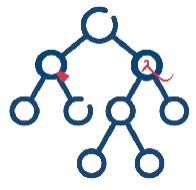
\includegraphics[height=1.0cm]{msca_logo.png}}%
    \end{center}

    \vspace{0.6cm}

    % Main title with Q logos on sides (with clickable links)
    \begin{center}
        \begin{minipage}{0.1\textwidth}
            \centering
            \href{https://quantlet.com}{
\includegraphics[height=1.1cm]{ql_logo.png}}
        \end{minipage}%
        \begin{minipage}{0.78\textwidth}
            \centering
            {\LARGE\bfseries\usebeamercolor[fg]{title}\inserttitle}

            \vspace{0.3cm}

            {\usebeamerfont{subtitle}\usebeamercolor[fg]{title}\insertsubtitle}
        \end{minipage}%
        \begin{minipage}{0.1\textwidth}
            \centering
            \href{https://quantinar.com}{
\includegraphics[height=1.1cm]{qr_logo.png}}
        \end{minipage}
    \end{center}

    \vspace{0.6cm}

    % Authors (left aligned)
    \hspace{0.5cm}{\usebeamerfont{author}\insertauthor}

    \vspace{0.3cm}

    % Institute/Affiliations (left aligned)
    \hspace{0.5cm}\begin{minipage}[t]{0.9\textwidth}
        \raggedright\small\insertinstitute
    \end{minipage}
}

%=============================================================================
% THEOREM ENVIRONMENTS
%=============================================================================
\theoremstyle{definition}
\setbeamertemplate{theorems}[numbered]
\ifdefined\atslang
\newtheorem{defn}{Definiție}
\newtheorem{thm}{Teoremă}
\newtheorem{prop}{Propoziție}
\newtheorem{rmk}{Observație}
\else
\newtheorem{defn}{Definition}
\newtheorem{thm}{Theorem}
\newtheorem{prop}{Proposition}
\newtheorem{rmk}{Remark}
\fi

%=============================================================================
% CENTRED MINIPAGE (no extra vertical space)
%=============================================================================
\newenvironment{cminipage}[1]{%
    \par\noindent\hfill\begin{minipage}{#1}\ignorespaces
}{%
    \end{minipage}\hfill\null\par
}

%=============================================================================
% CUSTOM COMMANDS
%=============================================================================
\newcommand{\E}{\mathbb{E}}
\newcommand{\Var}{\text{Var}}
\newcommand{\Cov}{\text{Cov}}
\newcommand{\Corr}{\text{Corr}}
\newcommand{\R}{\mathbb{R}}
\newcommand{\N}{\mathbb{N}}
\newcommand{\Z}{\mathbb{Z}}
\newcommand{\B}{\mathbf{B}}
\newcommand{\imark}{\textcolor{MainBlue}{\textbullet}}
\newcommand{\RMSE}{\text{RMSE}}
\newcommand{\MAE}{\text{MAE}}
\newcommand{\MAPE}{\text{MAPE}}

% Boldface vector/matrix commands (VAR, VECM, state space)
\newcommand{\bY}{\mathbf{Y}}
\newcommand{\bX}{\mathbf{X}}
\newcommand{\bA}{\mathbf{A}}
\newcommand{\bB}{\mathbf{B}}
\newcommand{\bepsilon}{\boldsymbol{\varepsilon}}
\newcommand{\bSigma}{\boldsymbol{\Sigma}}
\newcommand{\bPhi}{\boldsymbol{\Phi}}
\newcommand{\bGamma}{\boldsymbol{\Gamma}}
\newcommand{\bPi}{\boldsymbol{\Pi}}
\newcommand{\bc}{\mathbf{c}}
\newcommand{\balpha}{\boldsymbol{\alpha}}
\newcommand{\bbeta}{\boldsymbol{\beta}}
\newcommand{\bvarepsilon}{\boldsymbol{\varepsilon}}

% Seminar marks
\newcommand{\correct}{\textcolor{Forest}{\checkmark}}
\newcommand{\incorrect}{\textcolor{Crimson}{\texttimes}}
 se definește
%   \newcommand{\coursename}{Advanced Time Series Analysis and Forecasting}          (EN)
%   \newcommand{\coursename}{Analiza avansată a seriilor de timp și previziune}       (RO)  și  \def\atslang{ro}
% Fișierele .tex se află în EN/Courses, EN/Seminars, RO/Cursuri, RO/Seminarii (două niveluri sub rădăcină).
% Deck-urile sînt generate de latex/build_chapterN.py / build_seminarN.py (vezi latex/ats_build.py).

\documentclass[9pt, aspectratio=169, t]{beamer}
\providecommand{\coursename}{Advanced Time Series Analysis and Forecasting}

% Ensure content fits on slides
\setbeamersize{text margin left=8mm, text margin right=8mm}
% Smaller institute font (title page)
\setbeamerfont{institute}{size=\footnotesize}

%=============================================================================
% THEME AND STYLE CONFIGURATION
%=============================================================================
\usetheme{default}
% Using default theme for clean header/footer control

% Color Palette (matching Redispatch PDF)
\definecolor{MainBlue}{RGB}{26, 58, 110}
\definecolor{AccentBlue}{RGB}{26, 58, 110}
\definecolor{IDAred}{RGB}{205, 0, 0}
\definecolor{DarkGray}{RGB}{51, 51, 51}
\definecolor{MediumGray}{RGB}{128, 128, 128}
\definecolor{LightGray}{RGB}{248, 248, 248}
\definecolor{VeryLightGray}{RGB}{235, 235, 235}
\definecolor{KeynoteGray}{RGB}{218, 218, 218}
\definecolor{SectionGray}{RGB}{120, 120, 120}
\definecolor{FooterGray}{RGB}{100, 100, 100}
\definecolor{Crimson}{RGB}{220, 53, 69}
\definecolor{Forest}{RGB}{46, 125, 50}
\definecolor{Amber}{RGB}{181, 133, 63}
\definecolor{Orange}{RGB}{230, 126, 34}
\definecolor{Purple}{RGB}{142, 68, 173}

% Gradient background (exact Keynote 315° gradient: white to RGB 218,218,218)
\setbeamertemplate{background}{%
    \begin{tikzpicture}[remember picture, overlay]
        \shade[shading=axis, shading angle=315,
        top color=white, bottom color=KeynoteGray]
        (current page.south west) rectangle (current page.north east);
    \end{tikzpicture}%
}
% Fallback solid color for compatibility
\setbeamercolor{background canvas}{bg=}

\setbeamercolor{palette primary}{bg=MainBlue, fg=white}
\setbeamercolor{palette secondary}{bg=MainBlue!85, fg=white}
\setbeamercolor{palette tertiary}{bg=MainBlue!70, fg=white}
\setbeamercolor{structure}{fg=MainBlue}
\setbeamercolor{title}{fg=IDAred}
\setbeamercolor{frametitle}{fg=IDAred, bg=}
\setbeamercolor{block title}{bg=MainBlue, fg=white}
\setbeamercolor{block body}{bg=VeryLightGray, fg=DarkGray}
\setbeamercolor{block title alerted}{bg=Crimson, fg=white}
\setbeamercolor{block body alerted}{bg=Crimson!8, fg=DarkGray}
\setbeamercolor{block title example}{bg=Forest, fg=white}
\setbeamercolor{block body example}{bg=Forest!8, fg=DarkGray}
\setbeamercolor{item}{fg=MainBlue}

% Footer colors (override Madrid theme blue)
\setbeamercolor{author in head/foot}{fg=FooterGray, bg=}
\setbeamercolor{title in head/foot}{fg=FooterGray, bg=}
\setbeamercolor{date in head/foot}{fg=FooterGray, bg=}
\setbeamercolor{section in head/foot}{fg=FooterGray, bg=}
\setbeamercolor{subsection in head/foot}{fg=FooterGray, bg=}

% Bullet styles (apply everywhere including blocks)
\setbeamertemplate{itemize item}{\color{MainBlue}$\boxdot$}
\setbeamertemplate{itemize subitem}{\color{MainBlue}$\blacktriangleright$}
\setbeamertemplate{itemize subsubitem}{\color{MainBlue}\tiny$\bullet$}
\setbeamertemplate{itemize/enumerate body begin}{\normalsize}
\setbeamertemplate{itemize/enumerate subbody begin}{\normalsize}

% Item spacing - compact style
\setlength{\leftmargini}{10pt}       % Level 1: minimal indent
\setlength{\leftmarginii}{10pt}      % Level 2: minimal additional indent
% Compact list spacing (zero extra space before/after lists in blocks)
\makeatletter
\def\@listi{\leftmargin\leftmargini \topsep 0pt \parsep 0pt \itemsep 0pt}
\def\@listii{\leftmargin\leftmarginii \topsep 0pt \parsep 0pt \itemsep 0pt}
\makeatother

\setbeamertemplate{navigation symbols}{}

%=============================================================================
% CUSTOM HEADLINE
%=============================================================================
\setbeamertemplate{headline}{%
    \vskip10pt%
    \hbox to \paperwidth{%
        \hskip0.5cm%
        {\small\color{FooterGray}\renewcommand{\hyperlink}[2]{##2}\insertsectionhead}%
        \hfill%
        \textcolor{FooterGray}{\small\insertframenumber}%
        \hskip0.5cm%
    }%
    \vskip4pt%
    {\color{FooterGray}\hrule height 0.4pt}%
}

%=============================================================================
% CUSTOM FOOTER
%=============================================================================
\usepackage{fontawesome5}

\setbeamertemplate{footline}{%
    {\color{FooterGray}\hrule height 0.4pt}%
    \vskip4pt%
    \hbox to \paperwidth{%
        \hskip0.5cm%
        \textcolor{FooterGray}{\small\coursename}%
        \hfill%
        \raisebox{-0.1em}{%
            \begin{tikzpicture}[x=0.08em, y=0.08em, line width=0.4pt]
                \draw[FooterGray] (0,3) -- (1,4) -- (2,3.5) -- (3,5) -- (4,4) -- (5,6) -- (6,5.5) -- (7,4) -- (8,5) -- (9,7) -- (10,6) -- (11,5) -- (12,6.5) -- (13,8) -- (14,7) -- (15,6) -- (16,7.5) -- (17,9) -- (18,8) -- (19,7) -- (20,8.5) -- (21,10) -- (22,9) -- (23,8) -- (24,9.5);
            \end{tikzpicture}%
        }%
        \hskip0.5cm%
    }%
    \vskip6pt%
}

%=============================================================================
% PACKAGES
%=============================================================================
\usepackage[utf8]{inputenc}
\DeclareUnicodeCharacter{03B1}{\ensuremath{\alpha}}
\usepackage[T1]{fontenc}
\usepackage{amsmath, amssymb, amsthm}
\usepackage{mathtools}
\usepackage{bm}
\usepackage{tikz}
\usetikzlibrary{arrows.meta, positioning, shapes, calc, decorations.pathreplacing, shadings}
\usepackage{booktabs}
\usepackage{multirow}
\usepackage{array}
\usepackage{graphicx}
\usepackage{animate}
\usepackage{hyperref}
\usepackage{colortbl}
\usepackage{listings}
\lstset{language=Python, basicstyle=\ttfamily\scriptsize, keywordstyle=\color{MainBlue}\bfseries,
  commentstyle=\color{Forest}, stringstyle=\color{Crimson}, breaklines=true,
  frame=none, backgroundcolor=\color{VeryLightGray}, xleftmargin=2mm}
\hypersetup{colorlinks=true, linkcolor=MainBlue, urlcolor=MainBlue}
\graphicspath{{../../logos/}{../../charts/}{../../photos/}}
\usepackage{xcolor}
\hfuzz=2pt  % Suppress tiny overfull warnings (<2pt)
\vfuzz=2pt  % Suppress tiny vertical overfull warnings (<2pt)

%=============================================================================
% QUANTLET COMMANDS
%   \quantlet{<displayed name>}{<url>}       (generic)
%   \atsquantlet{Ch_05}{ATS_ch5_garch}       -> https://github.com/danpele/Advanced-Time-Series/tree/main/Quantlets/Ch_05/ATS_ch5_garch
%   \qlurl{<folder>} is defined per chapter by the generator (Quantlets/Ch_NN/<folder>)
%=============================================================================
\newcommand{\atsrepo}{https://github.com/danpele/Advanced-Time-Series}
\newcommand{\atsqlbase}{https://github.com/danpele/Advanced-Time-Series/tree/main/Quantlets}
\newcommand{\quantlet}[2]{%
    \hfill\href{#2}{%
        \raisebox{-0.15em}{
\includegraphics[height=0.7em]{ql_logo.png}}%
        \textcolor{MainBlue}{\tiny\ #1}%
    }%
}
\newcommand{\atsquantlet}[2]{\quantlet{\detokenize{#2}}{\atsqlbase/#1/#2}}

%=============================================================================
% NOTEBOOKS (Google Colab)
%   \colaburl{notebooks/EN/chapter5_seminar_notebook.ipynb} -> the Colab link of a file in the ATS repo
%   \nb: the chapter notebook (each seminar deck redefines it with \renewcommand)
%=============================================================================
\newcommand{\colaburl}[1]{https://colab.research.google.com/github/danpele/Advanced-Time-Series/blob/main/#1}
\newcommand{\nb}{https://colab.research.google.com/github/danpele/Advanced-Time-Series/tree/main/notebooks/EN}
\newcommand{\nbname}{notebooks/EN}

%=============================================================================
% SLIDE HELPERS (used by the generators; the same as in MFM)
%=============================================================================
% local font size for list bodies (the preamble forces \normalsize)
\newcommand{\itemsize}[1]{\setbeamertemplate{itemize/enumerate body begin}{#1}\setbeamertemplate{itemize/enumerate subbody begin}{#1}}
\newcommand{\intitle}[1]{{\hypersetup{urlcolor=white}#1}}   % white links inside coloured title bars
\newcommand{\imgcap}[1]{{\scriptsize #1}\\[0.5mm]}          % caption under a photo
\newcommand{\imgcredit}[2]{{\tiny\color{FooterGray}\href{#1}{#2}}}   % image credit: source URL, author/licence
\newcommand{\aiprompt}[1]{{\ttfamily\color{MainBlue}#1}}     % a prompt to an AI assistant

%=============================================================================
% SEMINARS: student version by default; the instructor wrapper *_solutions.tex sets \solutionstrue
%=============================================================================
\makeatletter\@ifundefined{ifsolutions}{\expandafter\newif\csname ifsolutions\endcsname}{}\makeatother
\newcommand{\solonly}[1]{\ifsolutions #1\fi}
\newcommand{\propsub}{\ifsolutions\else\framesubtitle{\ifdefined\atslang Rezolvarea se discută la seminar\else Solution discussed in class\fi}\fi}

%=============================================================================
% APPENDIX AND CHAPTER LINKS (latex/appendix_links.py writes the calls; it also re-declares these
% macros before \begin{document}, so the decks compile with or without this preamble block)
%=============================================================================
\providecommand{\atsapplink}[3]{\hypertarget{#2}{}\hyperlink{#1}{\beamergotobutton{#3}}}
\providecommand{\atsappback}[2]{\begin{tikzpicture}[remember picture,overlay]\node[anchor=south east] at ([xshift=-3mm,yshift=7mm]current page.south east){\hyperlink{#1}{\beamerreturnbutton{#2}}};\end{tikzpicture}}
\providecommand{\atschlink}[2]{\href{#1}{#2}}
\providecommand{\atschlinkt}[2]{\href{#1}{\usebeamercolor[fg]{frametitle}#2}}

%=============================================================================
% QUANTINAR COMMAND: link către un curs Quantinar (subiecte avansate)
%=============================================================================
\newcommand{\quantinar}[2]{%
    \href{#2}{%
        \raisebox{-0.15em}{
\includegraphics[height=0.8em]{qr_logo.png}}%
        \textcolor{MainBlue}{\scriptsize\ #1}%
    }%
}

%=============================================================================
% CUSTOM TITLE PAGE
%=============================================================================
\defbeamertemplate*{title page}{hybrid}[1][]
{
    \vspace{0.2cm}
    % Logos row - top header (with clickable links)
    \begin{center}
        \href{https://www.ase.ro}{
\includegraphics[height=1.0cm]{ase_logo.png}}\hspace{0.3cm}%
        \href{https://theida.net}{
\includegraphics[height=1.0cm]{ida_logo.png}}\hspace{0.3cm}%
        \href{https://blockchain-research-center.com}{
\includegraphics[height=1.0cm]{brc_logo.png}}\hspace{0.3cm}%
        \href{https://www.ai4efin.ase.ro}{
\includegraphics[height=1.0cm]{ai4efin_logo.png}}\hspace{0.3cm}%
        \href{https://ipe.ro/new}{
\includegraphics[height=1.0cm]{acad_logo.png}}\hspace{0.3cm}%
        \href{https://www.digital-finance-msca.com}{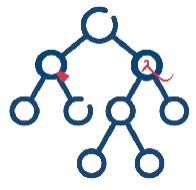
\includegraphics[height=1.0cm]{msca_logo.png}}%
    \end{center}

    \vspace{0.6cm}

    % Main title with Q logos on sides (with clickable links)
    \begin{center}
        \begin{minipage}{0.1\textwidth}
            \centering
            \href{https://quantlet.com}{
\includegraphics[height=1.1cm]{ql_logo.png}}
        \end{minipage}%
        \begin{minipage}{0.78\textwidth}
            \centering
            {\LARGE\bfseries\usebeamercolor[fg]{title}\inserttitle}

            \vspace{0.3cm}

            {\usebeamerfont{subtitle}\usebeamercolor[fg]{title}\insertsubtitle}
        \end{minipage}%
        \begin{minipage}{0.1\textwidth}
            \centering
            \href{https://quantinar.com}{
\includegraphics[height=1.1cm]{qr_logo.png}}
        \end{minipage}
    \end{center}

    \vspace{0.6cm}

    % Authors (left aligned)
    \hspace{0.5cm}{\usebeamerfont{author}\insertauthor}

    \vspace{0.3cm}

    % Institute/Affiliations (left aligned)
    \hspace{0.5cm}\begin{minipage}[t]{0.9\textwidth}
        \raggedright\small\insertinstitute
    \end{minipage}
}

%=============================================================================
% THEOREM ENVIRONMENTS
%=============================================================================
\theoremstyle{definition}
\setbeamertemplate{theorems}[numbered]
\ifdefined\atslang
\newtheorem{defn}{Definiție}
\newtheorem{thm}{Teoremă}
\newtheorem{prop}{Propoziție}
\newtheorem{rmk}{Observație}
\else
\newtheorem{defn}{Definition}
\newtheorem{thm}{Theorem}
\newtheorem{prop}{Proposition}
\newtheorem{rmk}{Remark}
\fi

%=============================================================================
% CENTRED MINIPAGE (no extra vertical space)
%=============================================================================
\newenvironment{cminipage}[1]{%
    \par\noindent\hfill\begin{minipage}{#1}\ignorespaces
}{%
    \end{minipage}\hfill\null\par
}

%=============================================================================
% CUSTOM COMMANDS
%=============================================================================
\newcommand{\E}{\mathbb{E}}
\newcommand{\Var}{\text{Var}}
\newcommand{\Cov}{\text{Cov}}
\newcommand{\Corr}{\text{Corr}}
\newcommand{\R}{\mathbb{R}}
\newcommand{\N}{\mathbb{N}}
\newcommand{\Z}{\mathbb{Z}}
\newcommand{\B}{\mathbf{B}}
\newcommand{\imark}{\textcolor{MainBlue}{\textbullet}}
\newcommand{\RMSE}{\text{RMSE}}
\newcommand{\MAE}{\text{MAE}}
\newcommand{\MAPE}{\text{MAPE}}

% Boldface vector/matrix commands (VAR, VECM, state space)
\newcommand{\bY}{\mathbf{Y}}
\newcommand{\bX}{\mathbf{X}}
\newcommand{\bA}{\mathbf{A}}
\newcommand{\bB}{\mathbf{B}}
\newcommand{\bepsilon}{\boldsymbol{\varepsilon}}
\newcommand{\bSigma}{\boldsymbol{\Sigma}}
\newcommand{\bPhi}{\boldsymbol{\Phi}}
\newcommand{\bGamma}{\boldsymbol{\Gamma}}
\newcommand{\bPi}{\boldsymbol{\Pi}}
\newcommand{\bc}{\mathbf{c}}
\newcommand{\balpha}{\boldsymbol{\alpha}}
\newcommand{\bbeta}{\boldsymbol{\beta}}
\newcommand{\bvarepsilon}{\boldsymbol{\varepsilon}}

% Seminar marks
\newcommand{\correct}{\textcolor{Forest}{\checkmark}}
\newcommand{\incorrect}{\textcolor{Crimson}{\texttimes}}
 se definește
%   \newcommand{\coursename}{Advanced Time Series Analysis and Forecasting}          (EN)
%   \newcommand{\coursename}{Analiza avansată a seriilor de timp și previziune}       (RO)  și  \def\atslang{ro}
% Fișierele .tex se află în EN/Courses, EN/Seminars, RO/Cursuri, RO/Seminarii (două niveluri sub rădăcină).
% Deck-urile sînt generate de latex/build_chapterN.py / build_seminarN.py (vezi latex/ats_build.py).

\documentclass[9pt, aspectratio=169, t]{beamer}
\providecommand{\coursename}{Advanced Time Series Analysis and Forecasting}

% Ensure content fits on slides
\setbeamersize{text margin left=8mm, text margin right=8mm}
% Smaller institute font (title page)
\setbeamerfont{institute}{size=\footnotesize}

%=============================================================================
% THEME AND STYLE CONFIGURATION
%=============================================================================
\usetheme{default}
% Using default theme for clean header/footer control

% Color Palette (matching Redispatch PDF)
\definecolor{MainBlue}{RGB}{26, 58, 110}
\definecolor{AccentBlue}{RGB}{26, 58, 110}
\definecolor{IDAred}{RGB}{205, 0, 0}
\definecolor{DarkGray}{RGB}{51, 51, 51}
\definecolor{MediumGray}{RGB}{128, 128, 128}
\definecolor{LightGray}{RGB}{248, 248, 248}
\definecolor{VeryLightGray}{RGB}{235, 235, 235}
\definecolor{KeynoteGray}{RGB}{218, 218, 218}
\definecolor{SectionGray}{RGB}{120, 120, 120}
\definecolor{FooterGray}{RGB}{100, 100, 100}
\definecolor{Crimson}{RGB}{220, 53, 69}
\definecolor{Forest}{RGB}{46, 125, 50}
\definecolor{Amber}{RGB}{181, 133, 63}
\definecolor{Orange}{RGB}{230, 126, 34}
\definecolor{Purple}{RGB}{142, 68, 173}

% Gradient background (exact Keynote 315° gradient: white to RGB 218,218,218)
\setbeamertemplate{background}{%
    \begin{tikzpicture}[remember picture, overlay]
        \shade[shading=axis, shading angle=315,
        top color=white, bottom color=KeynoteGray]
        (current page.south west) rectangle (current page.north east);
    \end{tikzpicture}%
}
% Fallback solid color for compatibility
\setbeamercolor{background canvas}{bg=}

\setbeamercolor{palette primary}{bg=MainBlue, fg=white}
\setbeamercolor{palette secondary}{bg=MainBlue!85, fg=white}
\setbeamercolor{palette tertiary}{bg=MainBlue!70, fg=white}
\setbeamercolor{structure}{fg=MainBlue}
\setbeamercolor{title}{fg=IDAred}
\setbeamercolor{frametitle}{fg=IDAred, bg=}
\setbeamercolor{block title}{bg=MainBlue, fg=white}
\setbeamercolor{block body}{bg=VeryLightGray, fg=DarkGray}
\setbeamercolor{block title alerted}{bg=Crimson, fg=white}
\setbeamercolor{block body alerted}{bg=Crimson!8, fg=DarkGray}
\setbeamercolor{block title example}{bg=Forest, fg=white}
\setbeamercolor{block body example}{bg=Forest!8, fg=DarkGray}
\setbeamercolor{item}{fg=MainBlue}

% Footer colors (override Madrid theme blue)
\setbeamercolor{author in head/foot}{fg=FooterGray, bg=}
\setbeamercolor{title in head/foot}{fg=FooterGray, bg=}
\setbeamercolor{date in head/foot}{fg=FooterGray, bg=}
\setbeamercolor{section in head/foot}{fg=FooterGray, bg=}
\setbeamercolor{subsection in head/foot}{fg=FooterGray, bg=}

% Bullet styles (apply everywhere including blocks)
\setbeamertemplate{itemize item}{\color{MainBlue}$\boxdot$}
\setbeamertemplate{itemize subitem}{\color{MainBlue}$\blacktriangleright$}
\setbeamertemplate{itemize subsubitem}{\color{MainBlue}\tiny$\bullet$}
\setbeamertemplate{itemize/enumerate body begin}{\normalsize}
\setbeamertemplate{itemize/enumerate subbody begin}{\normalsize}

% Item spacing - compact style
\setlength{\leftmargini}{10pt}       % Level 1: minimal indent
\setlength{\leftmarginii}{10pt}      % Level 2: minimal additional indent
% Compact list spacing (zero extra space before/after lists in blocks)
\makeatletter
\def\@listi{\leftmargin\leftmargini \topsep 0pt \parsep 0pt \itemsep 0pt}
\def\@listii{\leftmargin\leftmarginii \topsep 0pt \parsep 0pt \itemsep 0pt}
\makeatother

\setbeamertemplate{navigation symbols}{}

%=============================================================================
% CUSTOM HEADLINE
%=============================================================================
\setbeamertemplate{headline}{%
    \vskip10pt%
    \hbox to \paperwidth{%
        \hskip0.5cm%
        {\small\color{FooterGray}\renewcommand{\hyperlink}[2]{##2}\insertsectionhead}%
        \hfill%
        \textcolor{FooterGray}{\small\insertframenumber}%
        \hskip0.5cm%
    }%
    \vskip4pt%
    {\color{FooterGray}\hrule height 0.4pt}%
}

%=============================================================================
% CUSTOM FOOTER
%=============================================================================
\usepackage{fontawesome5}

\setbeamertemplate{footline}{%
    {\color{FooterGray}\hrule height 0.4pt}%
    \vskip4pt%
    \hbox to \paperwidth{%
        \hskip0.5cm%
        \textcolor{FooterGray}{\small\coursename}%
        \hfill%
        \raisebox{-0.1em}{%
            \begin{tikzpicture}[x=0.08em, y=0.08em, line width=0.4pt]
                \draw[FooterGray] (0,3) -- (1,4) -- (2,3.5) -- (3,5) -- (4,4) -- (5,6) -- (6,5.5) -- (7,4) -- (8,5) -- (9,7) -- (10,6) -- (11,5) -- (12,6.5) -- (13,8) -- (14,7) -- (15,6) -- (16,7.5) -- (17,9) -- (18,8) -- (19,7) -- (20,8.5) -- (21,10) -- (22,9) -- (23,8) -- (24,9.5);
            \end{tikzpicture}%
        }%
        \hskip0.5cm%
    }%
    \vskip6pt%
}

%=============================================================================
% PACKAGES
%=============================================================================
\usepackage[utf8]{inputenc}
\DeclareUnicodeCharacter{03B1}{\ensuremath{\alpha}}
\usepackage[T1]{fontenc}
\usepackage{amsmath, amssymb, amsthm}
\usepackage{mathtools}
\usepackage{bm}
\usepackage{tikz}
\usetikzlibrary{arrows.meta, positioning, shapes, calc, decorations.pathreplacing, shadings}
\usepackage{booktabs}
\usepackage{multirow}
\usepackage{array}
\usepackage{graphicx}
\usepackage{animate}
\usepackage{hyperref}
\usepackage{colortbl}
\usepackage{listings}
\lstset{language=Python, basicstyle=\ttfamily\scriptsize, keywordstyle=\color{MainBlue}\bfseries,
  commentstyle=\color{Forest}, stringstyle=\color{Crimson}, breaklines=true,
  frame=none, backgroundcolor=\color{VeryLightGray}, xleftmargin=2mm}
\hypersetup{colorlinks=true, linkcolor=MainBlue, urlcolor=MainBlue}
\graphicspath{{../../logos/}{../../charts/}{../../photos/}}
\usepackage{xcolor}
\hfuzz=2pt  % Suppress tiny overfull warnings (<2pt)
\vfuzz=2pt  % Suppress tiny vertical overfull warnings (<2pt)

%=============================================================================
% QUANTLET COMMANDS
%   \quantlet{<displayed name>}{<url>}       (generic)
%   \atsquantlet{Ch_05}{ATS_ch5_garch}       -> https://github.com/danpele/Advanced-Time-Series/tree/main/Quantlets/Ch_05/ATS_ch5_garch
%   \qlurl{<folder>} is defined per chapter by the generator (Quantlets/Ch_NN/<folder>)
%=============================================================================
\newcommand{\atsrepo}{https://github.com/danpele/Advanced-Time-Series}
\newcommand{\atsqlbase}{https://github.com/danpele/Advanced-Time-Series/tree/main/Quantlets}
\newcommand{\quantlet}[2]{%
    \hfill\href{#2}{%
        \raisebox{-0.15em}{
\includegraphics[height=0.7em]{ql_logo.png}}%
        \textcolor{MainBlue}{\tiny\ #1}%
    }%
}
\newcommand{\atsquantlet}[2]{\quantlet{\detokenize{#2}}{\atsqlbase/#1/#2}}

%=============================================================================
% NOTEBOOKS (Google Colab)
%   \colaburl{notebooks/EN/chapter5_seminar_notebook.ipynb} -> the Colab link of a file in the ATS repo
%   \nb: the chapter notebook (each seminar deck redefines it with \renewcommand)
%=============================================================================
\newcommand{\colaburl}[1]{https://colab.research.google.com/github/danpele/Advanced-Time-Series/blob/main/#1}
\newcommand{\nb}{https://colab.research.google.com/github/danpele/Advanced-Time-Series/tree/main/notebooks/EN}
\newcommand{\nbname}{notebooks/EN}

%=============================================================================
% SLIDE HELPERS (used by the generators; the same as in MFM)
%=============================================================================
% local font size for list bodies (the preamble forces \normalsize)
\newcommand{\itemsize}[1]{\setbeamertemplate{itemize/enumerate body begin}{#1}\setbeamertemplate{itemize/enumerate subbody begin}{#1}}
\newcommand{\intitle}[1]{{\hypersetup{urlcolor=white}#1}}   % white links inside coloured title bars
\newcommand{\imgcap}[1]{{\scriptsize #1}\\[0.5mm]}          % caption under a photo
\newcommand{\imgcredit}[2]{{\tiny\color{FooterGray}\href{#1}{#2}}}   % image credit: source URL, author/licence
\newcommand{\aiprompt}[1]{{\ttfamily\color{MainBlue}#1}}     % a prompt to an AI assistant

%=============================================================================
% SEMINARS: student version by default; the instructor wrapper *_solutions.tex sets \solutionstrue
%=============================================================================
\makeatletter\@ifundefined{ifsolutions}{\expandafter\newif\csname ifsolutions\endcsname}{}\makeatother
\newcommand{\solonly}[1]{\ifsolutions #1\fi}
\newcommand{\propsub}{\ifsolutions\else\framesubtitle{\ifdefined\atslang Rezolvarea se discută la seminar\else Solution discussed in class\fi}\fi}

%=============================================================================
% APPENDIX AND CHAPTER LINKS (latex/appendix_links.py writes the calls; it also re-declares these
% macros before \begin{document}, so the decks compile with or without this preamble block)
%=============================================================================
\providecommand{\atsapplink}[3]{\hypertarget{#2}{}\hyperlink{#1}{\beamergotobutton{#3}}}
\providecommand{\atsappback}[2]{\begin{tikzpicture}[remember picture,overlay]\node[anchor=south east] at ([xshift=-3mm,yshift=7mm]current page.south east){\hyperlink{#1}{\beamerreturnbutton{#2}}};\end{tikzpicture}}
\providecommand{\atschlink}[2]{\href{#1}{#2}}
\providecommand{\atschlinkt}[2]{\href{#1}{\usebeamercolor[fg]{frametitle}#2}}

%=============================================================================
% QUANTINAR COMMAND: link către un curs Quantinar (subiecte avansate)
%=============================================================================
\newcommand{\quantinar}[2]{%
    \href{#2}{%
        \raisebox{-0.15em}{
\includegraphics[height=0.8em]{qr_logo.png}}%
        \textcolor{MainBlue}{\scriptsize\ #1}%
    }%
}

%=============================================================================
% CUSTOM TITLE PAGE
%=============================================================================
\defbeamertemplate*{title page}{hybrid}[1][]
{
    \vspace{0.2cm}
    % Logos row - top header (with clickable links)
    \begin{center}
        \href{https://www.ase.ro}{
\includegraphics[height=1.0cm]{ase_logo.png}}\hspace{0.3cm}%
        \href{https://theida.net}{
\includegraphics[height=1.0cm]{ida_logo.png}}\hspace{0.3cm}%
        \href{https://blockchain-research-center.com}{
\includegraphics[height=1.0cm]{brc_logo.png}}\hspace{0.3cm}%
        \href{https://www.ai4efin.ase.ro}{
\includegraphics[height=1.0cm]{ai4efin_logo.png}}\hspace{0.3cm}%
        \href{https://ipe.ro/new}{
\includegraphics[height=1.0cm]{acad_logo.png}}\hspace{0.3cm}%
        \href{https://www.digital-finance-msca.com}{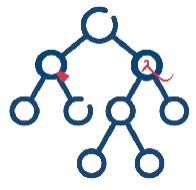
\includegraphics[height=1.0cm]{msca_logo.png}}%
    \end{center}

    \vspace{0.6cm}

    % Main title with Q logos on sides (with clickable links)
    \begin{center}
        \begin{minipage}{0.1\textwidth}
            \centering
            \href{https://quantlet.com}{
\includegraphics[height=1.1cm]{ql_logo.png}}
        \end{minipage}%
        \begin{minipage}{0.78\textwidth}
            \centering
            {\LARGE\bfseries\usebeamercolor[fg]{title}\inserttitle}

            \vspace{0.3cm}

            {\usebeamerfont{subtitle}\usebeamercolor[fg]{title}\insertsubtitle}
        \end{minipage}%
        \begin{minipage}{0.1\textwidth}
            \centering
            \href{https://quantinar.com}{
\includegraphics[height=1.1cm]{qr_logo.png}}
        \end{minipage}
    \end{center}

    \vspace{0.6cm}

    % Authors (left aligned)
    \hspace{0.5cm}{\usebeamerfont{author}\insertauthor}

    \vspace{0.3cm}

    % Institute/Affiliations (left aligned)
    \hspace{0.5cm}\begin{minipage}[t]{0.9\textwidth}
        \raggedright\small\insertinstitute
    \end{minipage}
}

%=============================================================================
% THEOREM ENVIRONMENTS
%=============================================================================
\theoremstyle{definition}
\setbeamertemplate{theorems}[numbered]
\ifdefined\atslang
\newtheorem{defn}{Definiție}
\newtheorem{thm}{Teoremă}
\newtheorem{prop}{Propoziție}
\newtheorem{rmk}{Observație}
\else
\newtheorem{defn}{Definition}
\newtheorem{thm}{Theorem}
\newtheorem{prop}{Proposition}
\newtheorem{rmk}{Remark}
\fi

%=============================================================================
% CENTRED MINIPAGE (no extra vertical space)
%=============================================================================
\newenvironment{cminipage}[1]{%
    \par\noindent\hfill\begin{minipage}{#1}\ignorespaces
}{%
    \end{minipage}\hfill\null\par
}

%=============================================================================
% CUSTOM COMMANDS
%=============================================================================
\newcommand{\E}{\mathbb{E}}
\newcommand{\Var}{\text{Var}}
\newcommand{\Cov}{\text{Cov}}
\newcommand{\Corr}{\text{Corr}}
\newcommand{\R}{\mathbb{R}}
\newcommand{\N}{\mathbb{N}}
\newcommand{\Z}{\mathbb{Z}}
\newcommand{\B}{\mathbf{B}}
\newcommand{\imark}{\textcolor{MainBlue}{\textbullet}}
\newcommand{\RMSE}{\text{RMSE}}
\newcommand{\MAE}{\text{MAE}}
\newcommand{\MAPE}{\text{MAPE}}

% Boldface vector/matrix commands (VAR, VECM, state space)
\newcommand{\bY}{\mathbf{Y}}
\newcommand{\bX}{\mathbf{X}}
\newcommand{\bA}{\mathbf{A}}
\newcommand{\bB}{\mathbf{B}}
\newcommand{\bepsilon}{\boldsymbol{\varepsilon}}
\newcommand{\bSigma}{\boldsymbol{\Sigma}}
\newcommand{\bPhi}{\boldsymbol{\Phi}}
\newcommand{\bGamma}{\boldsymbol{\Gamma}}
\newcommand{\bPi}{\boldsymbol{\Pi}}
\newcommand{\bc}{\mathbf{c}}
\newcommand{\balpha}{\boldsymbol{\alpha}}
\newcommand{\bbeta}{\boldsymbol{\beta}}
\newcommand{\bvarepsilon}{\boldsymbol{\varepsilon}}

% Seminar marks
\newcommand{\correct}{\textcolor{Forest}{\checkmark}}
\newcommand{\incorrect}{\textcolor{Crimson}{\texttimes}}


\newcommand{\qlurl}[1]{https://github.com/danpele/Advanced-Time-Series/tree/main/Quantlets/Ch_06/#1}

% Clickable citations (DOIs verified via Crossref)
\newcommand{\refAG}{\href{https://doi.org/10.1086/511283}{Aguiar and Gopinath (2007)}}
\newcommand{\refADH}{\href{https://doi.org/10.1111/j.1467-9868.2009.00736.x}{Andrieu, Doucet and Holenstein (2010)}}
\newcommand{\refAR}{\href{https://doi.org/10.1214/07-AOS574}{Andrieu and Roberts (2009)}}
\newcommand{\refAK}{\href{https://doi.org/10.1214/aos/1176349739}{Ansley and Kohn (1985)}}
\newcommand{\refBM}{\href{https://doi.org/10.1002/jae.2306}{Bańbura and Modugno (2014)}}
\newcommand{\refBN}{\href{https://doi.org/10.1016/0304-3932(81)90040-4}{Beveridge and Nelson (1981)}}
\newcommand{\refBol}{\href{https://doi.org/10.1016/0304-4076(86)90063-1}{Bollerslev (1986)}}
\newcommand{\refBro}{\href{https://doi.org/10.1214/14-AOAS788}{Brodersen et al.\ (2015)}}
\newcommand{\refCK}{\href{https://doi.org/10.1093/biomet/81.3.541}{Carter and Kohn (1994)}}
\newcommand{\refCJ}{\href{https://doi.org/10.1504/IJMMNO.2009.030090}{Chan and Jeliazkov (2009)}}
\newcommand{\refCP}{\href{https://doi.org/10.1007/978-3-030-47845-2}{Chopin and Papaspiliopoulos (2020)}}
\newcommand{\refCla}{\href{https://doi.org/10.2307/1884282}{Clark (1987)}}
\newcommand{\refCSa}{\href{https://doi.org/10.1086/654451}{Cogley and Sargent (2001)}}
\newcommand{\refCSb}{\href{https://doi.org/10.1016/j.red.2004.10.009}{Cogley and Sargent (2005)}}
\newcommand{\refdJa}{\href{https://doi.org/10.1214/aos/1176348139}{de Jong (1991)}}
\newcommand{\refdJS}{\href{https://doi.org/10.1093/biomet/82.2.339}{de Jong and Shephard (1995)}}
\newcommand{\refDM}{\href{https://doi.org/10.1007/978-1-4684-9393-1}{Del Moral (2004)}}
\newcommand{\refDNP}{\href{https://doi.org/10.1093/restud/rdv024}{Del Negro and Primiceri (2015)}}
\newcommand{\refDPDK}{\href{https://doi.org/10.1093/biomet/asu075}{Doucet, Pitt, Deligiannidis and Kohn (2015)}}
\newcommand{\refDGR}{\href{https://doi.org/10.1016/j.jeconom.2011.02.012}{Doz, Giannone and Reichlin (2011)}}
\newcommand{\refDKa}{\href{https://doi.org/10.1093/biomet/89.3.603}{Durbin and Koopman (2002)}}
\newcommand{\refDK}{\href{https://doi.org/10.1093/acprof:oso/9780199641178.001.0001}{Durbin and Koopman (2012)}}
\newcommand{\refFS}{\href{https://doi.org/10.1111/j.1467-9892.1994.tb00184.x}{Frühwirth-Schnatter (1994)}}
\newcommand{\refFSW}{\href{https://doi.org/10.1016/j.jeconom.2009.07.003}{Frühwirth-Schnatter and Wagner (2010)}}
\newcommand{\refGRS}{\href{https://doi.org/10.1016/j.jmoneco.2008.05.010}{Giannone, Reichlin and Small (2008)}}
\newcommand{\refGSS}{\href{https://doi.org/10.1049/ip-f-2.1993.0015}{Gordon, Salmond and Smith (1993)}}
\newcommand{\refHam}{\href{https://doi.org/10.2307/j.ctv14jx6sm}{Hamilton (1994)}}
\newcommand{\refHamB}{\href{https://doi.org/10.1162/rest_a_00706}{Hamilton (2018)}}
\newcommand{\refHar}{\href{https://doi.org/10.1017/CBO9781107049994}{Harvey (1990)}}
\newcommand{\refHJ}{\href{https://doi.org/10.1002/jae.3950080302}{Harvey and Jaeger (1993)}}
\newcommand{\refHRS}{\href{https://doi.org/10.2307/2297980}{Harvey, Ruiz and Shephard (1994)}}
\newcommand{\refJPR}{\href{https://doi.org/10.1080/07350015.1994.10524553}{Jacquier, Polson and Rossi (1994)}}
\newcommand{\refJU}{\href{https://doi.org/10.1109/JPROC.2003.823141}{Julier and Uhlmann (2004)}}
\newcommand{\refJK}{\href{https://doi.org/10.1111/ectj.12029}{Jungbacker and Koopman (2015)}}
\newcommand{\refKal}{\href{https://doi.org/10.1115/1.3662552}{Kalman (1960)}}
\newcommand{\refKMW}{\href{https://doi.org/10.1162/REST_a_00691}{Kamber, Morley and Wong (2018)}}
\newcommand{\refKN}{\href{https://doi.org/10.7551/mitpress/6444.001.0001}{Kim and Nelson (1999)}}
\newcommand{\refKSC}{\href{https://doi.org/10.1111/1467-937X.00050}{Kim, Shephard and Chib (1998)}}
\newcommand{\refKit}{\href{https://doi.org/10.1080/10618600.1996.10474692}{Kitagawa (1996)}}
\newcommand{\refKoo}{\href{https://doi.org/10.1080/01621459.1997.10473685}{Koopman (1997)}}
\newcommand{\refKD}{\href{https://doi.org/10.1111/1467-9892.00186}{Koopman and Durbin (2000)}}
\newcommand{\refMM}{\href{https://doi.org/10.1002/jae.695}{Mariano and Murasawa (2003)}}
\newcommand{\refMNZ}{\href{https://doi.org/10.1162/003465303765299765}{Morley, Nelson and Zivot (2003)}}
\newcommand{\refOCSN}{\href{https://doi.org/10.1016/j.jeconom.2006.07.008}{Omori, Chib, Shephard and Nakajima (2007)}}
\newcommand{\refOvN}{\href{https://doi.org/10.1162/003465302760556422}{Orphanides and van Norden (2002)}}
\newcommand{\refPet}{\href{https://doi.org/10.1016/j.ijforecast.2021.11.001}{Petropoulos et al.\ (2022)}}
\newcommand{\refPS}{\href{https://doi.org/10.1080/01621459.1999.10474153}{Pitt and Shephard (1999)}}
\newcommand{\refPSGK}{\href{https://doi.org/10.1016/j.jeconom.2012.06.004}{Pitt, Silva, Giordani and Kohn (2012)}}
\newcommand{\refPri}{\href{https://doi.org/10.1111/j.1467-937X.2005.00353.x}{Primiceri (2005)}}
\newcommand{\refSV}{\href{https://doi.org/10.1504/IJMMNO.2014.059942}{Scott and Varian (2014)}}
\newcommand{\refSH}{\href{https://doi.org/10.1111/j.1467-9892.1990.tb00062.x}{Shephard and Harvey (1990)}}
\newcommand{\refSS}{\href{https://doi.org/10.1111/j.1467-9892.1982.tb00349.x}{Shumway and Stoffer (1982)}}
\newcommand{\refSWa}{\href{https://doi.org/10.1080/01621459.1998.10474116}{Stock and Watson (1998)}}
\newcommand{\refSWb}{\href{https://doi.org/10.1111/j.1538-4616.2007.00014.x}{Stock and Watson (2007)}}
\newcommand{\refTay}{\href{https://doi.org/10.1111/j.1467-9965.1994.tb00057.x}{Taylor (1994)}}
\newcommand{\refWat}{\href{https://doi.org/10.1016/0304-3932(86)90054-1}{Watson (1986)}}

\title[Advanced Time Series Analysis and Forecasting]{Advanced Time Series Analysis and Forecasting}
\subtitle{Chapter 6: State space models and Bayesian filtering}
\author[D.T. Pele]{Daniel Traian PELE}
\institute{Bucharest University of Economic Studies\\
IDA Institute Digital Assets\\
Blockchain Research Center\\
AI4EFin Artificial Intelligence for Energy Finance\\
Romanian Academy, Institute for Economic Forecasting\\
MSCA Digital Finance}
\date{}

%=============================================================================
\providecommand{\atsapplink}[3]{\hypertarget{#2}{}\hyperlink{#1}{\beamergotobutton{#3}}}  % APPLINKS-MACROS
\providecommand{\atsappback}[2]{\begin{tikzpicture}[remember picture,overlay]\node[anchor=south east] at ([xshift=-3mm,yshift=7mm]current page.south east){\hyperlink{#1}{\beamerreturnbutton{#2}}};\end{tikzpicture}}  % APPLINKS-MACROS
\providecommand{\atschlink}[2]{\href{#1}{#2}}  % APPLINKS-MACROS
\providecommand{\atschlinkt}[2]{\href{#1}{\usebeamercolor[fg]{frametitle}#2}}  % APPLINKS-MACROS
\begin{document}
%=============================================================================

{
\setbeamertemplate{headline}{}
\setbeamertemplate{footline}{}
\begin{frame}[noframenumbering]
    \titlepage
\end{frame}
}
% BEGIN-ACRONYMS (generat de latex/acronyms.py; nu editati manual)
\begin{frame}{Acronyms used in this material (1/3)}
\setbeamertemplate{itemize/enumerate body begin}{\tiny}
\begin{columns}[T]
\begin{column}{0.49\textwidth}
\begin{itemize}\setlength{\itemsep}{0pt}
    \item \textbf{AI}: Artificial Intelligence
    \item \textbf{APF}: Auxiliary Particle Filter
    \item \textbf{AR}: AutoRegressive (model); in event studies: Abnormal Return
    \item \textbf{ARCH}: AutoRegressive Conditional Heteroskedasticity
    \item \textbf{ARIMA}: AutoRegressive Integrated Moving Average (model)
    \item \textbf{ARMA}: AutoRegressive Moving Average (model)
    \item \textbf{BET}: Bucharest Exchange Trading (index)
    \item \textbf{BN}: Beveridge–Nelson (decomposition)
    \item \textbf{BNR}: Banca Națională a României (the National Bank of Romania)
    \item \textbf{BSTS}: Bayesian Structural Time Series
    \item \textbf{CI}: Confidence Interval
    \item \textbf{CLT}: Central Limit Theorem
    \item \textbf{CMRMTSPL}: Real manufacturing and trade industries sales (FRED series code)
\end{itemize}
\end{column}
\begin{column}{0.49\textwidth}
\begin{itemize}\setlength{\itemsep}{0pt}
    \item \textbf{DFM}: Dynamic Factor Model
    \item \textbf{DK}: Durbin–Koopman (simulation smoother, 2002)
    \item \textbf{DSGE}: Dynamic Stochastic General Equilibrium (model)
    \item \textbf{EKF}: Extended Kalman Filter
    \item \textbf{EM}: Expectation–Maximisation (algorithm)
    \item \textbf{EODHD}: EOD Historical Data (market-data provider)
    \item \textbf{ETS}: Error, Trend, Seasonality (exponential smoothing state space models)
    \item \textbf{FERMIAC}: mechanical Monte Carlo device of Enrico Fermi (Los Alamos, 1947)
    \item \textbf{FFBS}: Forward Filtering, Backward Sampling
    \item \textbf{FRED}: Federal Reserve Economic Data
    \item \textbf{GARCH}: Generalised AutoRegressive Conditional Heteroskedasticity
    \item \textbf{GDP}: Gross Domestic Product
    \item \textbf{GDPC1}: Real Gross Domestic Product (FRED code)
\end{itemize}
\end{column}
\end{columns}
\end{frame}
\begin{frame}{Acronyms used in this material (2/3)}
\setbeamertemplate{itemize/enumerate body begin}{\tiny}
\begin{columns}[T]
\begin{column}{0.49\textwidth}
\begin{itemize}\setlength{\itemsep}{0pt}
    \item \textbf{GDPDEF}: GDP implicit price deflator (FRED series code)
    \item \textbf{HICP}: Harmonised Index of Consumer Prices
    \item \textbf{HP}: Hodrick–Prescott (filter)
    \item \textbf{IG}: inverse gamma (distribution)
    \item \textbf{IMA}: Integrated Moving Average (model)
    \item \textbf{INDPRO}: Industrial production index (FRED series code)
    \item \textbf{KSC}: Kim–Shephard–Chib (1998), mixture sampler for stochastic volatility
    \item \textbf{LLM}: Large Language Model
    \item \textbf{LR}: Likelihood Ratio (test)
    \item \textbf{MA}: Moving Average
    \item \textbf{MCMC}: Markov Chain Monte Carlo
    \item \textbf{ML}: Machine Learning
    \item \textbf{MNZ}: Morley–Nelson–Zivot (2003)
\end{itemize}
\end{column}
\begin{column}{0.49\textwidth}
\begin{itemize}\setlength{\itemsep}{0pt}
    \item \textbf{OLS}: Ordinary Least Squares
    \item \textbf{PAYEMS}: Total nonfarm payroll employment (FRED series code)
    \item \textbf{PMMH}: Particle Marginal Metropolis–Hastings
    \item \textbf{QML}: Quasi-Maximum Likelihood
    \item \textbf{SMC}: Sequential Monte Carlo
    \item \textbf{SV}: Stochastic Volatility
    \item \textbf{TSA}: Time Series Analysis
    \item \textbf{TVP}: Time-Varying Parameter(s)
    \item \textbf{TVP-VAR}: Time-Varying-Parameter Vector AutoRegression
    \item \textbf{TVP-VAR-SV}: TVP-VAR with Stochastic Volatility
    \item \textbf{UC}: Unobserved Components (model)
    \item \textbf{UC-SV}: Unobserved Components model with Stochastic Volatility (Stock–Watson 2007)
    \item \textbf{UC-UR}: UC model with correlated trend and cycle shocks (Morley–Nelson–Zivot 2003)
\end{itemize}
\end{column}
\end{columns}
\end{frame}
\begin{frame}{Acronyms used in this material (3/3)}
\setbeamertemplate{itemize/enumerate body begin}{\tiny}
\begin{columns}[T]
\begin{column}{0.49\textwidth}
\begin{itemize}\setlength{\itemsep}{0pt}
    \item \textbf{UC0}: UC model with uncorrelated trend and cycle shocks (Clark 1987)
    \item \textbf{UKF}: Unscented Kalman Filter
    \item \textbf{US}: United States
    \item \textbf{VAR}: Vector AutoRegression
    \item \textbf{VAT}: Value Added Tax
    \item \textbf{W875RX1}: Real personal income excluding current transfer receipts (FRED series code)
\end{itemize}
\end{column}
\begin{column}{0.49\textwidth}
\end{column}
\end{columns}
\end{frame}
% END-ACRONYMS

\begin{frame}{Today's question and route}
\itemsize{\small}
\begin{itemize}
    \item \textbf{Question}: how do we learn about quantities we never observe (trend inflation, the output gap, volatility, time-varying coefficients) and how much should we trust what we learn?
    \begin{itemize}
        \item one framework: a state equation for the hidden quantity, a measurement equation for the data, and a filter that updates beliefs as data arrive
    \end{itemize}
    \item \textbf{Route} of the chapter
    \begin{itemize}
        \item the general linear Gaussian model, exact diffuse initialisation, the exact likelihood and inference at the boundary
        \item Bayesian state space: simulation smoothers and Gibbs sampling; stochastic volatility
        \item nonlinear filters: extended and unscented Kalman filters, particle filters, particle MCMC
        \item time-varying parameters, dynamic factors, trend--cycle decompositions and trend inflation with stochastic volatility
    \end{itemize}
    \item We build on \atschlink{https://danpele.github.io/Time-Series-Analysis/EN/Courses/chapter10_state_space_kalman_markov_switching.pdf}{TSA, Chapter 10} (state space form, Kalman filter by hand, smoothing, local level and trend, the UC output gap, Markov switching basics); Seminar 6 comes before this lecture
\end{itemize}
\end{frame}

\begin{frame}{Learning outcomes}
\itemsize{\small}
\begin{itemize}
    \item Derive the Kalman filter and smoother for the general linear Gaussian model, with exact diffuse initialisation, and write them in \texttt{numpy}
    \item Maximise the exact likelihood and judge inference on variances that may sit on the boundary (pile-up, bootstrap LR tests)
    \item Sample states with the Carter--Kohn, Durbin--Koopman and precision samplers inside a Gibbs sampler; estimate stochastic volatility by the KSC mixture
    \item Run extended, unscented and particle filters; use the particle likelihood in PMMH and choose the number of particles
    \item Estimate TVP regressions, UC models with correlated shocks and UC-SV trend inflation, and report how fragile the latent estimates are
\end{itemize}
\end{frame}

\begin{frame}{Reading, data and tools}
\itemsize{\small}
\begin{itemize}
    \item Backbone: \refDK, Ch.~2--9 and 11--14; \refHar; \refKN; \refHam, Ch.~13; \refCP
    \begin{itemize}
        \item original papers: \refKal, \refKoo, \refCK, \refDKa, \refKSC, \refGSS, \refPS, \refADH, \refPri, \refMNZ, \refSWb
    \end{itemize}
    \item Python Quantlets of this chapter: \href{https://github.com/danpele/Advanced-Time-Series/tree/main/Quantlets/Ch_06}{Quantlets/Ch\_06}
    \begin{itemize}
        \item Kalman filter and smoother with exact diffuse initialisation, simulation smoothers, KSC Gibbs sampler, bootstrap and auxiliary particle filters, PMMH and UC-SV written out in \texttt{numpy}; checked against \texttt{statsmodels}
    \end{itemize}
    \item Lecture notebook: \href{\colaburl{notebooks/EN/chapter6_lecture_notebook.ipynb}}{open in Google Colab}
\end{itemize}
\end{frame}

\begin{frame}{Data used in this chapter}
\itemsize{\footnotesize}
\begin{center}
\scriptsize
\begin{tabular}{>{\raggedright\arraybackslash}p{5.0cm}>{\raggedright\arraybackslash}p{4.4cm}>{\raggedright\arraybackslash}p{2.5cm}}
\toprule
\textbf{Series} & \textbf{Source} & \textbf{Use} \\
\midrule
US GDP price deflator, real GDP (quarterly) & FRED (GDPDEF, GDPC1) & likelihood, MNZ, UC-SV \\
S\&P 500 and BET, daily closes & EODHD & stochastic volatility \\
HICP of Romania and of the euro area (monthly index, 2025 = 100) & Eurostat prc\_hicp\_minr & TVP, UC-SV \\
Romanian real GDP, seasonally and calendar adjusted & Eurostat namq\_10\_gdp & output gap \\
US industrial production, payrolls, real income less transfers, real sales (monthly) & FRED (INDPRO, PAYEMS, W875RX1, CMRMTSPL) & DFM \\
\bottomrule
\end{tabular}
\end{center}
\begin{itemize}
    \item All sources are public and need no account or key; quarterly series to 2026Q2, monthly series to August or September 2026, daily data to 18 September 2026
    \item HICP: harmonised index of consumer prices; DFM: dynamic factor model
\end{itemize}
\end{frame}

\begin{frame}{From Apollo navigation to trend inflation}
\itemsize{\footnotesize}
\begin{columns}[T]
\begin{column}{0.36\textwidth}
\centering
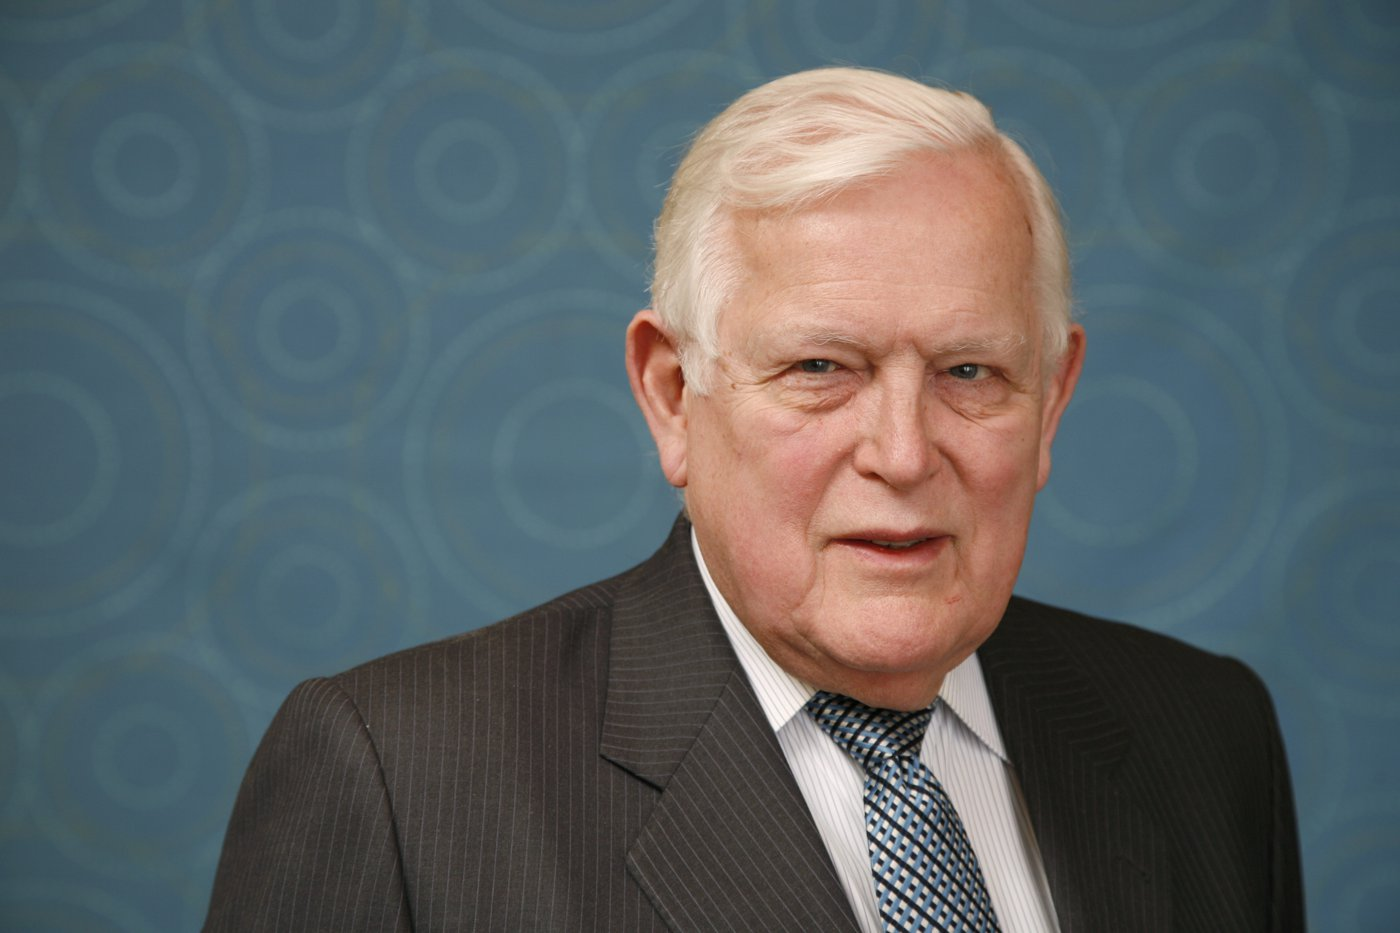
\includegraphics[height=0.36\textheight]{ch6_kalman_2007.jpg}\\[1mm]
\imgcap{Rudolf E. Kálmán, 2007}
\imgcredit{https://commons.wikimedia.org/wiki/File:ETH-BIB-Kalman,_Rudolf_E._(1930-2016)-HK_04-01925.jpg}{Photo: ETH-Bibliothek Zürich, Bildarchiv (2007); CC BY-SA 4.0; Wikimedia Commons}
\end{column}
\begin{column}{0.62\textwidth}
\begin{itemize}
    \item 1960: \refKal\ gives the recursive linear filter; it guides the Apollo missions within a decade
    \item 1982--1997: EM for state space models \refSS; structural time series \refHar; exact diffuse filtering \refKoo
    \item 1993--1999: particle filters \refGSS, \refPS; Gibbs sampling of states \refCK, \refFS; stochastic volatility \refKSC
    \item 2002--2010: the simulation smoother \refDKa; TVP-VAR with stochastic volatility \refPri, \refCSb; particle MCMC \refADH
    \item Today: central banks track trend inflation and the output gap with these tools \refSWb, \refMNZ
\end{itemize}
\end{column}
\end{columns}
\end{frame}


%=============================================================================
\section{The general linear Gaussian model}
%=============================================================================

\begin{frame}{From TSA to this chapter}
\itemsize{\small}
\begin{itemize}
    \item Known (\atschlink{https://danpele.github.io/Time-Series-Analysis/EN/Courses/chapter10_state_space_kalman_markov_switching.pdf}{TSA, Chapter 10}): the state space form, the Kalman filter for the local level by hand, smoothing, ML by the prediction error decomposition, the HP filter as a smoother, Hamilton (2018), Markov switching
    \item New here
    \begin{itemize}
        \item the filter and smoother for any linear Gaussian model, with nonstationary states initialised exactly (not with a large variance)
        \item inference when a variance may be zero; Bayesian sampling of whole state paths
        \item nonlinear and non-Gaussian models: stochastic volatility, particle filters, particle MCMC
        \item applications at research level: MNZ, UC-SV, TVP regressions, the ragged edge of a DFM
    \end{itemize}
    \item Markov switching in depth: \atschlink{https://danpele.github.io/Advanced-Time-Series/EN/Courses/chapter7_regime_switching_models.pdf}{Chapter 7}; nowcasting with factors: \atschlink{https://danpele.github.io/Advanced-Time-Series/EN/Courses/chapter5_bvar_factor_models_nowcasting.pdf}{Chapter 5}
\end{itemize}
\end{frame}

\begin{frame}{The general state space form (1/2)}
\itemsize{\small}
\begin{itemize}
    \item Two equations: the data are a noisy linear function of an unobserved state, and the state follows a first-order linear dynamic \[ y_t = Z_t\alpha_t + \varepsilon_t, \qquad \alpha_{t+1} = c_t + T_t\alpha_t + R_t\eta_t, \qquad t = 1, \dots, n \]
    \item Notation
    \begin{itemize}
        \item $y_t$ ($p\times 1$): the observations; $\alpha_t$ ($m\times 1$): the state; $n$: the sample length
        \item $Z_t$ ($p\times m$): the measurement matrix; $T_t$ ($m\times m$): the transition matrix; $c_t$: a known intercept
        \item $\varepsilon_t \sim N(0, H_t)$: measurement noise; $\eta_t \sim N(0, Q_t)$: state shocks; $R_t$ ($m\times r$) selects the states that receive shocks
        \item $\varepsilon_t$ and $\eta_s$ are independent of each other and over time
    \end{itemize}
    \item Initial state $\alpha_1 \sim N(a_1, P_1)$
    \begin{itemize}
        \item nonstationary or unknown fixed elements: $P_1 = \kappa P_\infty + P_*$, $\kappa \to \infty$; $P_\infty$ marks the diffuse elements, $P_*$ the covariance of the others
    \end{itemize}
\end{itemize}
\end{frame}

\begin{frame}{The general state space form (2/2)}
\itemsize{\small}
\begin{itemize}
    \item The system matrices $Z_t, T_t, R_t, H_t, Q_t$ depend on parameters $\psi$; time variation in $Z_t$ gives regressions with time-varying coefficients
    \begin{itemize}
        \item ARMA, UC, TVP regressions, DFM, VAR with missing data, ETS: all are special cases \refDK
    \end{itemize}
    \item Notation for the estimates
    \begin{itemize}
        \item $Y_t = (y_1, \dots, y_t)$: the data up to $t$
        \item predicted state: $a_t = \E(\alpha_t | Y_{t-1})$, $P_t = \Var(\alpha_t | Y_{t-1})$; filtered: $a_{t|t}$, $P_{t|t}$ (after $y_t$)
        \item smoothed: $\hat\alpha_t = \E(\alpha_t | Y_n)$, $V_t = \Var(\alpha_t | Y_n)$ (all the data)
    \end{itemize}
\end{itemize}
\end{frame}

\begin{frame}{The Kalman filter from one lemma}
\itemsize{\small}
\begin{itemize}
    \item Lemma (conditioning of jointly normal vectors): if $(x, y)$ is Gaussian, $\E(x | y) = \mu_x + \Sigma_{xy}\Sigma_{yy}^{-1}(y - \mu_y)$, $\Var(x | y) = \Sigma_{xx} - \Sigma_{xy}\Sigma_{yy}^{-1}\Sigma_{yx}$
    \begin{itemize}
        \item $\mu_x$, $\mu_y$: the means; $\Sigma_{xy} = \Cov(x, y)$, $\Sigma_{yy} = \Var(y)$: the covariance blocks
        \item apply it to $x = \alpha_t$ and $y = y_t$, conditional on $Y_{t-1}$: $v_t = y_t - Z_ta_t$ is the new information (the prediction error)
    \end{itemize}
    \item Prediction-error variance $\Var(v_t | Y_{t-1}) = F_t = Z_tP_tZ_t' + H_t$; $\Cov(\alpha_t, v_t | Y_{t-1}) = P_tZ_t'$; $v_t$ is independent of $Y_{t-1}$
    \item Update: $a_{t|t} = a_t + P_tZ_t'F_t^{-1}v_t$, $P_{t|t} = P_t - P_tZ_t'F_t^{-1}Z_tP_t$
    \item Prediction: $a_{t+1} = c_t + T_ta_{t|t}$, $P_{t+1} = T_tP_{t|t}T_t' + R_tQ_tR_t'$
    \item Without normality the same recursions give the best \emph{linear} predictor (minimum mean square error among linear functions of $Y_t$)
\end{itemize}
\end{frame}

\begin{frame}{The filter in one pass}
\itemsize{\small}
\begin{itemize}
    \item $v_t = y_t - Z_ta_t$, $\quad F_t = Z_tP_tZ_t' + H_t$, $\quad K_t = T_tP_tZ_t'F_t^{-1}$ (Kalman gain), $\quad L_t = T_t - K_tZ_t$
    \item $a_{t+1} = c_t + T_ta_t + K_tv_t$, $\quad P_{t+1} = T_tP_tL_t' + R_tQ_tR_t'$
    \item Cost: $O(n(m^3 + p^3))$; with time-invariant matrices $P_t$ converges to the steady state of the Riccati equation
    \begin{itemize}
        \item $P_t$ and $K_t$ do not depend on $y$: they can be computed before the data arrive
    \end{itemize}
    \item Missing $y_t$: set $Z_t = 0$ (or drop the missing rows): $v_t$ and $K_t$ vanish and the filter only predicts
    \begin{itemize}
        \item mixed frequencies and the ragged edge of real-time data are therefore free (\atschlink{https://danpele.github.io/Advanced-Time-Series/EN/Courses/chapter5_bvar_factor_models_nowcasting.pdf}{Chapter 5})
    \end{itemize}
    \item Multivariate $y_t$ with diagonal $H_t$: process the $p$ elements one at a time (univariate treatment \refKD): no $p\times p$ inversion
\end{itemize}
\end{frame}

\begin{frame}{Smoothing: backward recursions}
\itemsize{\small}
\begin{itemize}
    \item State smoother \refDK: $r_{t-1} = Z_t'F_t^{-1}v_t + L_t'r_t$, $\quad N_{t-1} = Z_t'F_t^{-1}Z_t + L_t'N_tL_t$, $\quad r_n = 0$, $N_n = 0$
    \item $r_{t-1}$: a weighted sum of the innovations after $t$; $N_{t-1} = \Var(r_{t-1})$; then $\hat\alpha_t = a_t + P_tr_{t-1}$, $\quad V_t = P_t - P_tN_{t-1}P_t$
    \item $r_{t-1}$ is a weighted sum of future innovations: $\hat\alpha_t$ corrects $a_t$ by everything learned after $t$
    \item Disturbance smoother: $\hat\varepsilon_t = H_t(F_t^{-1}v_t - K_t'r_t)$, $\hat\eta_t = Q_tR_t'r_t$: auxiliary residuals for outliers and breaks, and the score of the likelihood
    \item Derivation from the same lemma, now conditioning on $v_t, \dots, v_n$, which are independent (\atsapplink{atsapp1}{atssrc1}{Appendix})
\end{itemize}
\end{frame}

\begin{frame}{Diffuse initialisation}
\itemsize{\footnotesize}
\begin{itemize}
    \item Random walks, trends and regression coefficients have no stationary distribution: $P_1 = \kappa P_\infty + P_*$, $\kappa \to \infty$
    \begin{itemize}
        \item ``big kappa'' ($\kappa = 10^6$--$10^7$) is an approximation with two failures: the likelihood contains $-\frac12\ln\kappa$ terms, and round-off errors grow with $\kappa$
    \end{itemize}
    \item Exact diffuse filter \refKoo, \refAK, \refdJa: expand $P_t = \kappa P_{\infty,t} + P_{*,t} + O(\kappa^{-1})$ and keep both parts while $P_{\infty,t} \ne 0$
    \begin{itemize}
        \item $F_{\infty,t}$, $F_{*,t}$: the diffuse and finite parts of $F_t$; $K^{(0)}_t$, $K^{(1)}_t$: the matching gains; $L^{(0)}_t = T_t - K^{(0)}_tZ_t$, $L^{(1)}_t = -K^{(1)}_tZ_t$
        \item univariate $y_t$, $F_{\infty,t} = Z_tP_{\infty,t}Z_t' > 0$: $K^{(0)}_t = T_tP_{\infty,t}Z_t'/F_{\infty,t}$, $K^{(1)}_t = T_t(P_{*,t}Z_t' - P_{\infty,t}Z_t'F_{*,t}/F_{\infty,t})/F_{\infty,t}$
        \item $a_{t+1} = c_t + T_ta_t + K^{(0)}_tv_t$; $P_{\infty,t+1} = T_tP_{\infty,t}L^{(0)\prime}_t$; $P_{*,t+1} = T_tP_{\infty,t}L^{(1)\prime}_t + T_tP_{*,t}L^{(0)\prime}_t + R_tQ_tR_t'$
    \end{itemize}
    \item $P_{\infty,t}$ reaches zero after $d$ steps ($d$ = number of diffuse elements, if they are identified); then the ordinary filter takes over
    \item The smoother has matching diffuse recursions for $r^{(0)}, r^{(1)}, N^{(0)}, N^{(1)}, N^{(2)}$ \refDK, Section 5.3; in the Quantlet both are checked against \texttt{statsmodels}
\end{itemize}
\end{frame}

\begin{frame}{Exact diffuse against big kappa}
\itemsize{\footnotesize}
\begin{center}
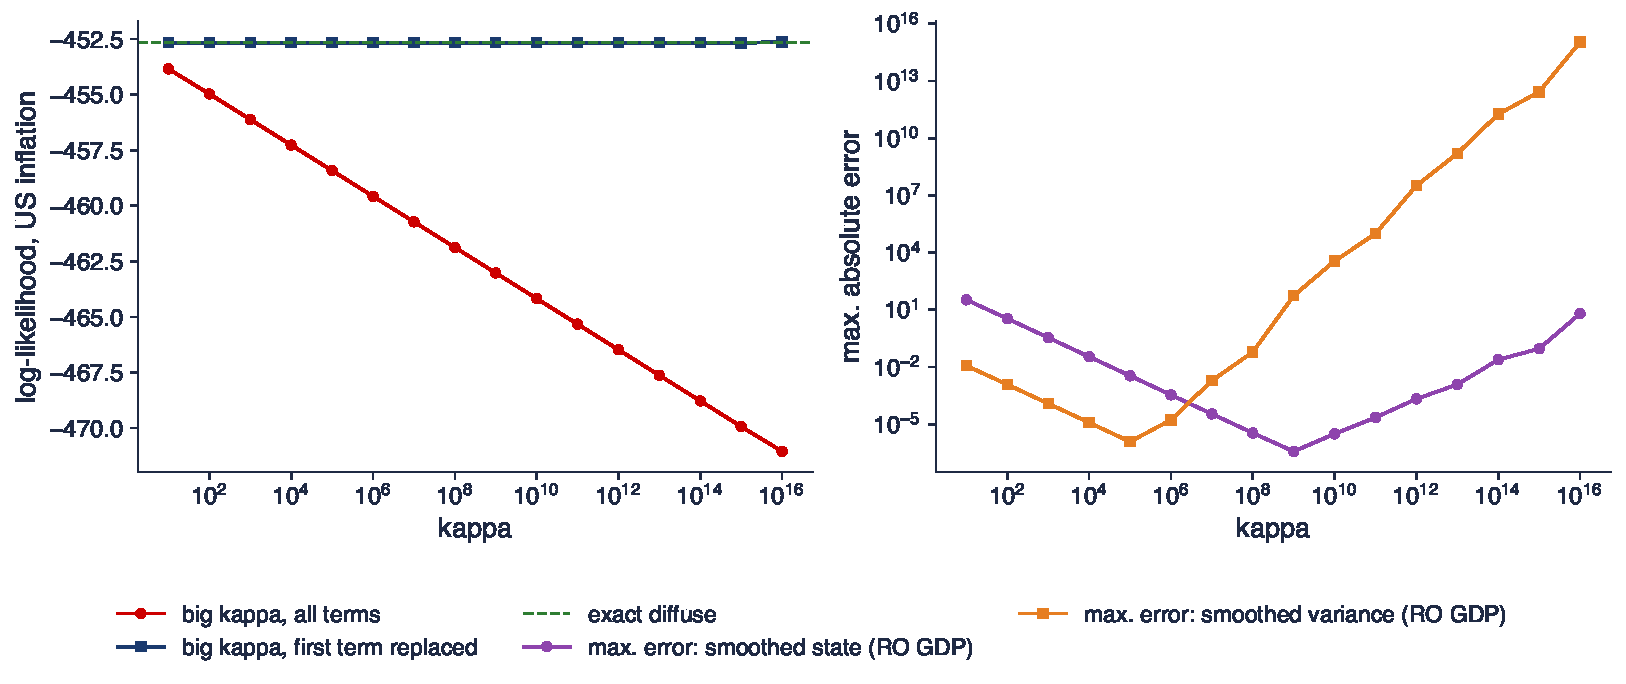
\includegraphics[width=0.97\textwidth,height=0.5\textheight,keepaspectratio]{ats_ch6_diffuse.pdf}
\end{center}
\vspace{-0.25cm}
\begin{itemize}
    \item Left: local level for US GDP-deflator inflation at the ML variances; right: local linear trend for 100$\times$log Romanian real GDP, $T = 106$; both against the exact diffuse filter
\end{itemize}
\quantlet{ATS\_ch6\_kalman\_mle}{\qlurl{ATS_ch6_kalman_mle}}
\end{frame}

\begin{frame}{Interpreting the diffuse initialisation}
\itemsize{\small}
\begin{itemize}
    \item With all terms, the big-kappa log-likelihood falls by $\frac12\ln 10$ per decade of $\kappa$: \ensuremath{-}460.72 at $\kappa = 10^7$, \ensuremath{-}468.78 at $10^{14}$; the exact value is \ensuremath{-}452.66
    \item Replacing the first term by its diffuse limit repairs the level (\ensuremath{-}452.66 at $10^7$), but only because $d = 1$ is known; ML over $\psi$ is unaffected, model comparison across different $d$ is not
    \item Smoothed variances: error 0.000012 at $\kappa = 10^4$, 0.06 at $10^8$ and $10^{15}$ at $10^{16}$: no single $\kappa$ is safe for both states and variances
    \item Practical rule: use the exact diffuse filter whenever the model has nonstationary or fixed unknown states
\end{itemize}
\end{frame}

\begin{frame}{Recap: The general linear Gaussian model}
\itemsize{\small}
\begin{itemize}
    \item One lemma (Gaussian conditioning) gives the filter, the smoother and the disturbance smoother
    \item Missing data, mixed frequencies and multivariate observations are handled inside the same recursions
    \item Nonstationary states need the exact diffuse filter; big kappa breaks the likelihood level and the smoothed variances
\end{itemize}
\end{frame}


%=============================================================================
\section{The exact likelihood and its maximisation}
%=============================================================================

\begin{frame}{The prediction error decomposition, diffuse case}
\itemsize{\small}
\begin{itemize}
    \item $p(y_1, \dots, y_n) = \prod_t p(y_t | Y_{t-1})$, and $y_t | Y_{t-1} \sim N(Z_ta_t, F_t)$: the likelihood is a by-product of the filter
    \item Diffuse log-likelihood \refDK, eq.~(7.4): $\ln L_d = -\frac{np}{2}\ln 2\pi - \frac12\sum_{t=1}^d w_t - \frac12\sum_{t=d+1}^n(\ln|F_t| + v_t'F_t^{-1}v_t)$
    \item $w_t = \ln F_{\infty,t}$ if $F_{\infty,t} > 0$, otherwise $w_t = \ln F_{*,t} + v_t^2/F_{*,t}$: the first $d$ observations only pin down the diffuse states
    \begin{itemize}
        \item equivalent to the marginal likelihood of \refdJa\ and to treating the diffuse states as fixed and concentrating them out
    \end{itemize}
    \item Scale: write $H_t = \sigma^2H^*_t$, $Q_t = \sigma^2Q^*_t$; then $F_t = \sigma^2F^*_t$ and $\hat\sigma^2 = \frac{1}{p(n - d)}\sum_{t>d}v_t'F_t^{*-1}v_t$: one parameter fewer in the numerical search
\end{itemize}
\end{frame}

\begin{frame}{Maximising the likelihood}
\itemsize{\small}
\begin{itemize}
    \item Parameterise variances as $\exp(\cdot)$, correlations as $\tanh(\cdot)$, AR coefficients through partial autocorrelations: unconstrained search, stationary models only
    \begin{itemize}
        \item several starting values: UC likelihoods are often multimodal (MNZ below)
    \end{itemize}
    \item Score in one filter-smoother pass: $\partial\ln L/\partial\psi = \frac12\sum_t\mathrm{tr}\{(\hat\varepsilon_t\hat\varepsilon_t' + \Var(\varepsilon_t|Y_n) - H_t)H_t^{-1}\tfrac{\partial H_t}{\partial\psi}H_t^{-1}\} + \dots$ \refDK, Section 7.3
    \item EM algorithm \refSS: the E-step is the smoother, the M-step has closed forms for $H$ and $Q$; slow near the optimum but robust from poor starts (large DFM)
    \item Standard errors: inverse Hessian at $\hat\psi$ (numerical); valid only for interior points; report them on the transformed scale
    \item Identification: some UC models are observationally equivalent to ARIMA models with fewer parameters; check the reduced form before interpreting the components
\end{itemize}
\end{frame}

\begin{frame}{Local level for US inflation: numpy against statsmodels}
\itemsize{\footnotesize}
\begin{center}
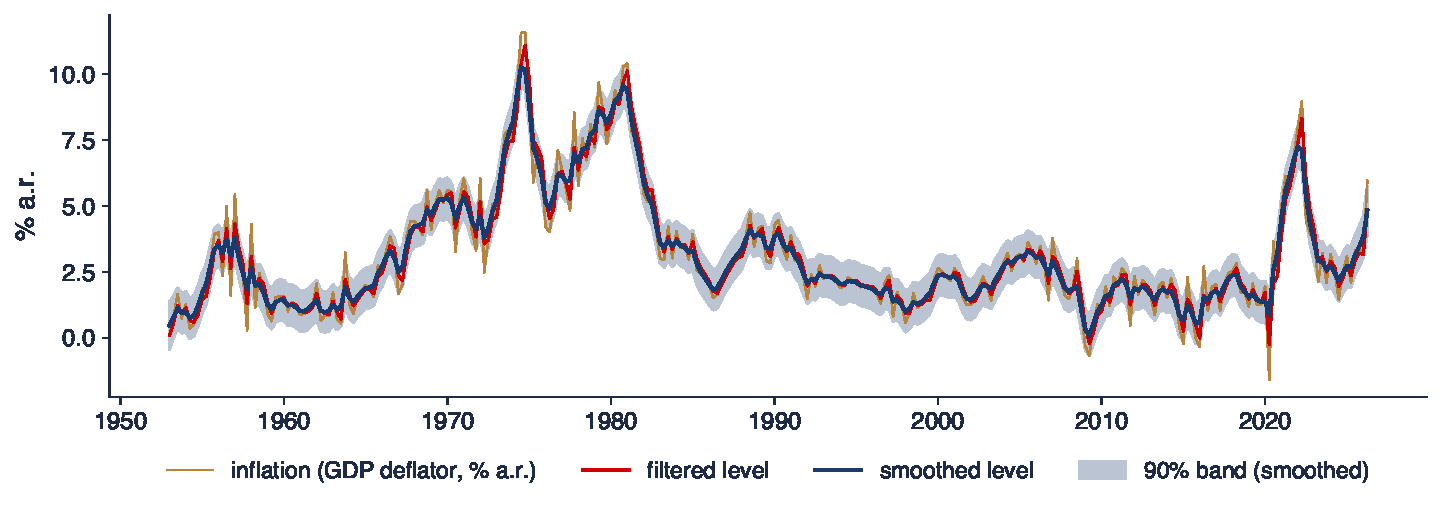
\includegraphics[width=0.97\textwidth,height=0.52\textheight,keepaspectratio]{ats_ch6_local_level.pdf}
\end{center}
\vspace{-0.25cm}
\begin{itemize}
    \item GDP-deflator inflation, 1953Q1--2026Q2, $T = 294$; exact diffuse ML; the smoothed level with a 90\% band and the one-sided (filtered) level
\end{itemize}
\quantlet{ATS\_ch6\_kalman\_mle}{\qlurl{ATS_ch6_kalman_mle}}
\end{frame}

\begin{frame}{Interpreting the local level estimates}
\itemsize{\small}
\begin{itemize}
    \item numpy: $\hat\sigma^2_\varepsilon = 0.517$, $\hat\sigma^2_\eta = 0.453$, $\hat q = 0.877$; statsmodels: 0.517 and 0.453: the same optimum
    \item Log-likelihoods \ensuremath{-}452.66 and \ensuremath{-}451.74: they differ by exactly $\frac12\ln 2\pi = 0.919$, the constant that \texttt{statsmodels} omits for the $d = 1$ diffuse observation
    \item Steady-state gain 0.596: each new quarter moves the level estimate by 60\% of the surprise; inflation is closer to a random walk than to white noise around a mean
    \item Last smoothed level 4.83\% (s.d. 0.55): at the end of the sample the smoothed and filtered estimates coincide, and so does their uncertainty
    \item One constant variance for 1953--2026 is implausible (Great Inflation, Great Moderation): this motivates UC-SV in the last section
\end{itemize}
\end{frame}

\begin{frame}{Inference at the boundary: the pile-up problem}
\itemsize{\small}
\begin{itemize}
    \item Local level with $q = \sigma^2_\eta/\sigma^2_\varepsilon$: the ML estimate equals exactly zero with positive probability even when $q > 0$ \refSH
    \begin{itemize}
        \item the score at $q = 0$ is often negative because a smooth trend fits the data better than a slightly wandering one
    \end{itemize}
    \item Consequences: the Hessian-based CI is invalid; the LR test of $q = 0$ is not $\chi^2_1$, not even $\frac12\chi^2_0 + \frac12\chi^2_1$, because the model under the alternative is nonstationary
    \begin{itemize}
        \item remedies: median-unbiased estimation of a coefficient variance \refSWa; parametric bootstrap of the LR statistic (TVP section); Bayesian priors that keep $q$ away from zero
    \end{itemize}
    \item Same issue in TVP regressions (is the coefficient constant?) and in UC models (is the trend deterministic?)
\end{itemize}
\end{frame}

\begin{frame}{How often is the estimated level variance exactly zero?}
\itemsize{\footnotesize}
\begin{center}
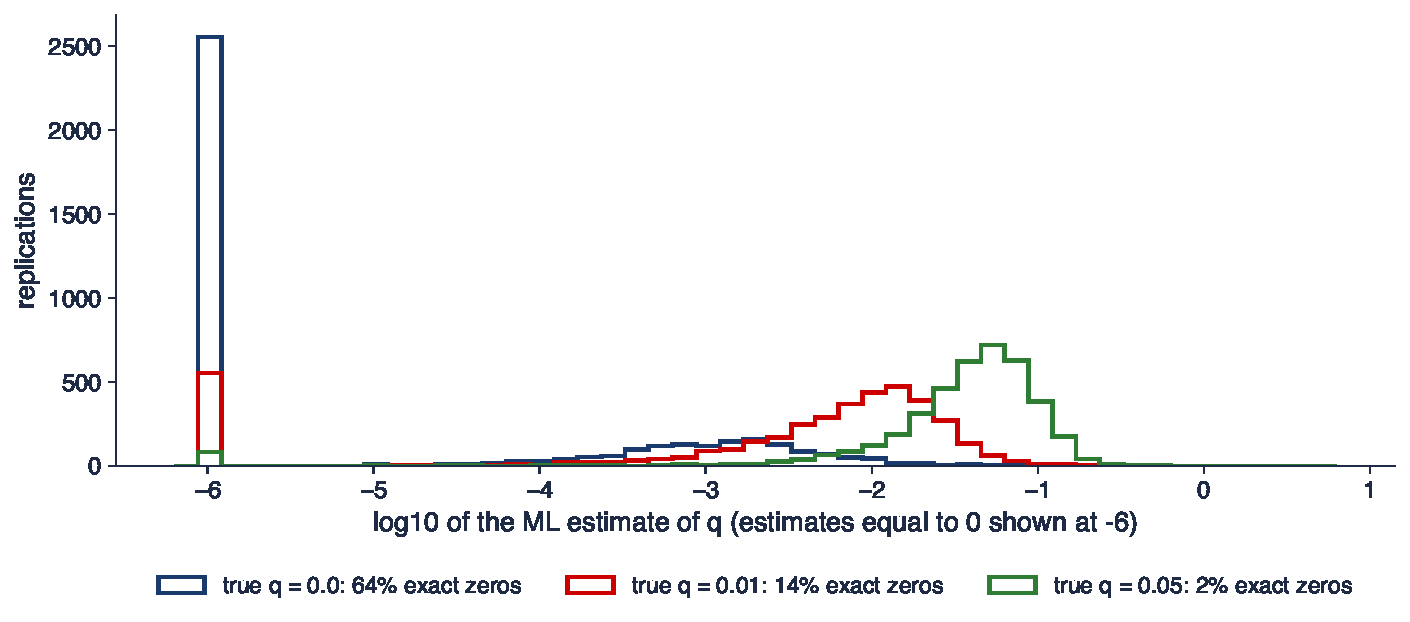
\includegraphics[width=0.97\textwidth,height=0.52\textheight,keepaspectratio]{ats_ch6_pileup.pdf}
\end{center}
\vspace{-0.25cm}
\begin{itemize}
    \item 4\,000 simulated local level series of length $T = 100$ for each true $q$; ML of $q$ on a fine grid with $\sigma^2_\varepsilon$ concentrated out
\end{itemize}
\quantlet{ATS\_ch6\_kalman\_mle}{\qlurl{ATS_ch6_kalman_mle}}
\end{frame}

\begin{frame}{Interpreting the pile-up simulation}
\itemsize{\small}
\begin{itemize}
    \item True $q = 0$: 64\% of the estimates are exactly zero; the rest spread over several orders of magnitude
    \item True $q = 0.01$: still 14\% zeros; median estimate 0.0077; with $q = 0.05$: 2\% zeros
    \item A reported $\hat\sigma^2_\eta = 0$ is therefore not evidence of a constant level; a small positive value is compatible with a deterministic one
    \item Report the profile likelihood or the posterior of $q$, not a point estimate with a Hessian standard error
\end{itemize}
\end{frame}

\begin{frame}{Recap: The exact likelihood}
\itemsize{\small}
\begin{itemize}
    \item The filter delivers the Gaussian likelihood; with diffuse states the first $d$ terms are replaced by their diffuse limits
    \item Concentrate the scale, parameterise without constraints, use several starts, and check the numbers against a second implementation
    \item Variances near zero pile up at zero: standard errors and $\chi^2$ tests fail at the boundary
\end{itemize}
\end{frame}


%=============================================================================
\section{Bayesian state space: simulation smoothing and Gibbs sampling}
%=============================================================================

\begin{frame}{Why sample the states?}
\itemsize{\footnotesize}
\begin{columns}[T]
\begin{column}{0.3\textwidth}
\centering
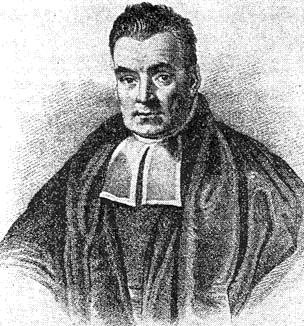
\includegraphics[height=0.34\textheight]{ch6_bayes.png}\\[1mm]
\imgcap{Portrait traditionally identified as Thomas Bayes (identification uncertain)}
\imgcredit{https://commons.wikimedia.org/wiki/File:Thomas_Bayes.gif}{Portrait: unknown author; public domain; Wikimedia Commons}
\end{column}
\begin{column}{0.68\textwidth}
\begin{itemize}
    \item Target: $p(\alpha_1, \dots, \alpha_n, \psi | Y_n)$; the filter gives $p(\alpha_t | Y_t, \psi)$ for one $t$ and one $\psi$ only
    \item Gibbs sampler: alternate $\alpha_{1:n} \sim p(\alpha_{1:n} | \psi, Y_n)$ and $\psi \sim p(\psi | \alpha_{1:n}, Y_n)$; given the states, $\psi$ is often a conjugate regression problem
    \item Uncertainty about $\psi$ enters the bands of the states (ML bands ignore it)
    \item Functions of whole paths become easy: the date of a peak, the probability that a trend stays inside a target band
    \item Sampling the whole path in one block (not $\alpha_t$ one at a time) is what makes the sampler mix
\end{itemize}
\end{column}
\end{columns}
\end{frame}

\begin{frame}{Forward filtering, backward sampling}
\itemsize{\small}
\begin{itemize}
    \item Factorisation: $p(\alpha_{1:n} | Y_n) = p(\alpha_n | Y_n)\prod_{t=1}^{n-1}p(\alpha_t | \alpha_{t+1}, Y_t)$ (Markov property of the state)
    \item Forward: run the filter, store $a_{t|t}, P_{t|t}$; draw $\alpha_n \sim N(a_{n|n}, P_{n|n})$ \refCK, \refFS
    \item Backward: $\alpha_t | \alpha_{t+1}, Y_t \sim N(m_t, S_t)$ by the lemma, with the smoothing gain $G_t = P_{t|t}T_t'P_{t+1}^{-1}$ ($m_t$, $S_t$: conditional mean and variance):
    \begin{itemize}
        \item $m_t = a_{t|t} + G_t(\alpha_{t+1} - c_t - T_ta_{t|t})$, $\quad S_t = P_{t|t} - G_tT_tP_{t|t}$
    \end{itemize}
    \item Issues: $P_{t+1}$ is singular when $R_tQ_tR_t'$ is (lags in the state): use the rows with shocks only; $n$ draws of dimension $m$
    \item Same output as the Gibbs step in the Bayesian VAR and DFM samplers of \atschlink{https://danpele.github.io/Advanced-Time-Series/EN/Courses/chapter5_bvar_factor_models_nowcasting.pdf}{Chapter 5}
\end{itemize}
\end{frame}

\begin{frame}{The Durbin--Koopman simulation smoother}
\itemsize{\small}
\begin{itemize}
    \item Idea \refDKa: $\alpha - \hat\alpha(y)$ has the same conditional distribution for every $y$ (Gaussian model): simulate it once from the model
    \item Algorithm (mean correction):
    \begin{itemize}
        \item 1. draw $\alpha^+_{1:n}, y^+_{1:n}$ from the model (shocks and initial state); keep the missing pattern of $y$
        \item 2. run one state smoother on $y - y^+$ (zero intercepts): $\hat\alpha(y - y^+) = \hat\alpha(y) - \hat\alpha(y^+)$
        \item 3. $\tilde\alpha = \alpha^+ + \hat\alpha(y) - \hat\alpha(y^+)$ is a draw from $p(\alpha | Y_n)$
    \end{itemize}
    \item Only the mean smoother is needed: no $P_{t|t}$ inversions, no singularity problems, diffuse states handled by the exact diffuse smoother
    \item Precursor: the disturbance simulation smoother of \refdJS; same idea for the disturbances $\varepsilon_t, \eta_t$
\end{itemize}
\end{frame}

\begin{frame}{The precision sampler}
\itemsize{\small}
\begin{itemize}
    \item Stack the model: $y = X\alpha + \varepsilon$, $H\alpha = \eta$ with $H$ a banded difference matrix: $\alpha | y \sim N(\hat\alpha, K^{-1})$, $K = H'\Sigma_\eta^{-1}H + X'\Sigma_\varepsilon^{-1}X$ \refCJ
    \item $K$ is banded (tridiagonal for a random walk): one banded Cholesky factor $K = U'U$ costs $O(n)$
    \begin{itemize}
        \item $\alpha$, $y$: all states and observations stacked; $X$: block-diagonal of the $Z_t$; $\Sigma_\varepsilon$, $\Sigma_\eta$: the stacked noise covariances; $K$: the posterior precision (inverse covariance)
        \item $\hat\alpha$ solves $K\hat\alpha = X'\Sigma_\varepsilon^{-1}y$; a draw is $\hat\alpha + U^{-1}z$, $z \sim N(0, I)$
    \end{itemize}
    \item Time-varying variances (stochastic volatility) only change the diagonal weights: ideal inside Gibbs samplers for UC-SV and SV
    \item Three samplers, one target: FFBS, DK and precision sampling draw from the same $p(\alpha | Y_n, \psi)$; they differ in cost and generality
\end{itemize}
\end{frame}

\begin{frame}{Three samplers of the same posterior}
\itemsize{\footnotesize}
\begin{center}
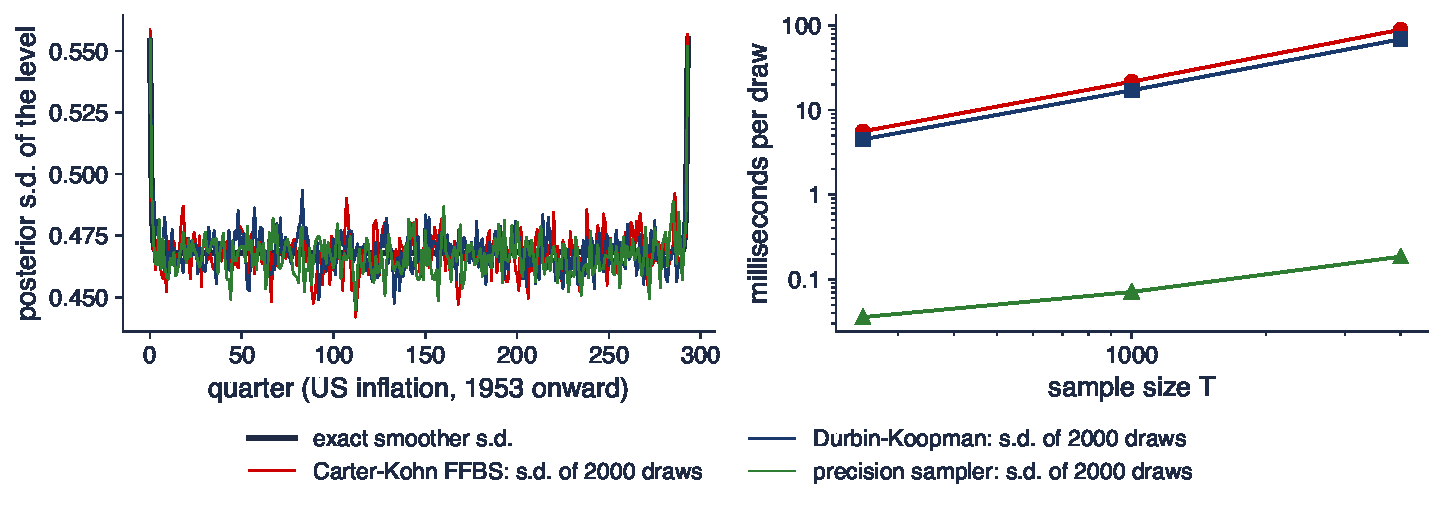
\includegraphics[width=0.97\textwidth,height=0.5\textheight,keepaspectratio]{ats_ch6_simsmoother.pdf}
\end{center}
\vspace{-0.25cm}
\begin{itemize}
    \item Local level for US inflation at the ML variances, proper prior $\mu_1 \sim N(y_1, 100)$; left: s.d. of 2\,000 draws against the exact smoother; right: time per draw for simulated samples
\end{itemize}
\quantlet{ATS\_ch6\_simulation\_smoother}{\qlurl{ATS_ch6_simulation_smoother}}
\end{frame}

\begin{frame}{Interpreting the three samplers}
\itemsize{\small}
\begin{itemize}
    \item Ratios of draw s.d. to exact s.d. lie in [0.94; 1.05] (FFBS), [0.96; 1.05] (DK) and [0.95; 1.04] (precision): Monte Carlo noise only
    \item Largest error of the draw means: 0.031, 0.027, 0.039, of the order of the Monte Carlo standard error
    \item For $T = 4000$: 89.2 ms (FFBS), 68.8 ms (DK), 0.19 ms (precision) per draw; all linear in $T$, the banded solver has no Python loop
    \item Choose DK for general models with diffuse states, precision sampling for random walks with time-varying variances
\end{itemize}
\end{frame}

\begin{frame}{A Gibbs sampler for the local level model}
\itemsize{\small}
\begin{itemize}
    \item Model: $y_t = \mu_t + \varepsilon_t$, $\mu_{t+1} = \mu_t + \eta_t$; $\mu_t$: the level; $IG(a_0, b_0)$: inverse gamma prior with shape $a_0$ and scale $b_0$; $q = \sigma^2_\eta/\sigma^2_\varepsilon$
    \item Block 1: $\mu_{1:n} | \sigma^2_\varepsilon, \sigma^2_\eta, Y_n$ by the DK simulation smoother (exact diffuse $\mu_1$)
    \item Block 2: $\sigma^2_\varepsilon | \mu, Y_n \sim IG(a_0 + \frac n2, b_0 + \frac12\sum_t(y_t - \mu_t)^2)$; $\sigma^2_\eta | \mu \sim IG(a_0 + \frac{n-1}{2}, b_0 + \frac12\sum_t(\Delta\mu_t)^2)$
    \item Prior $IG(2.5, 0.25)$ for both: proper, weak, and it rules out $\sigma^2_\eta = 0$ exactly
    \begin{itemize}
        \item the prior is not innocent near the boundary: a conjugate IG pushes small variances up; the non-centred parameterisation of \refFSW\ allows a normal prior on $\pm\sigma_\eta$ instead
    \end{itemize}
    \item Convergence: trace plots, several chains, inefficiency factor $1 + 2\sum_k\rho_k$ (Parzen weights): the number of draws worth one independent draw \refKSC
\end{itemize}
\end{frame}

\begin{frame}{Gibbs posterior of the signal-to-noise ratio}
\itemsize{\footnotesize}
\begin{center}
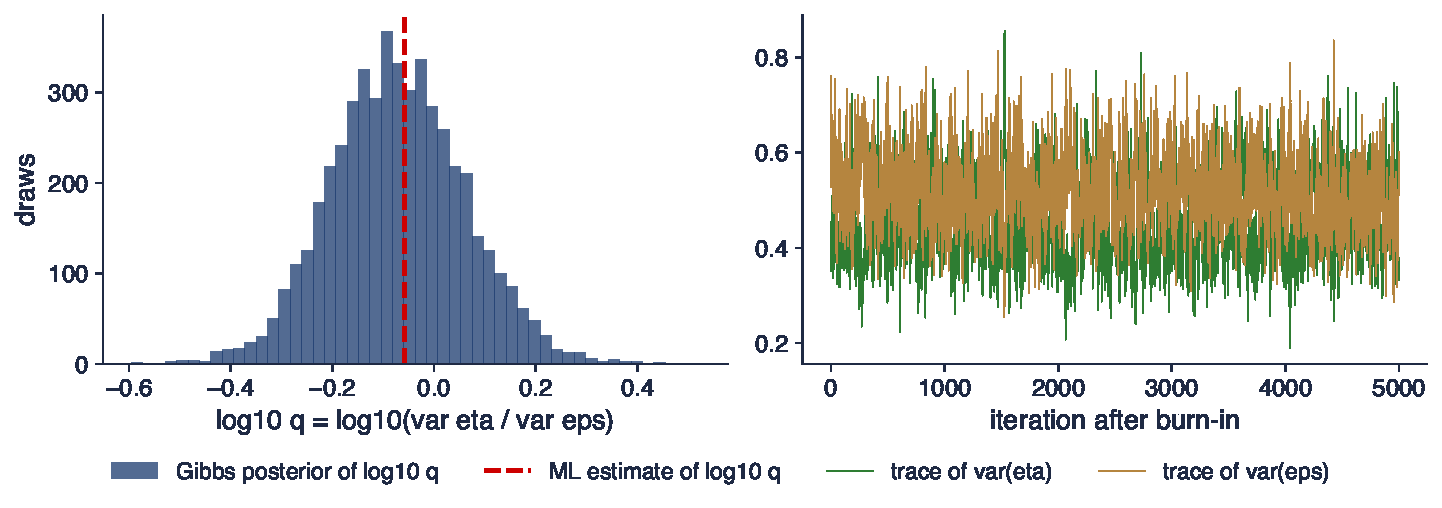
\includegraphics[width=0.97\textwidth,height=0.5\textheight,keepaspectratio]{ats_ch6_gibbs_ll.pdf}
\end{center}
\vspace{-0.25cm}
\begin{itemize}
    \item US inflation, local level, 5\,000 draws after burn-in; left: posterior of $\log_{10}q$ and the ML value; right: traces of the two variances
\end{itemize}
\quantlet{ATS\_ch6\_simulation\_smoother}{\qlurl{ATS_ch6_simulation_smoother}}
\end{frame}

\begin{frame}{Interpreting the Gibbs output}
\itemsize{\small}
\begin{itemize}
    \item Posterior median of $q$: 0.84, 90\% credible interval [0.52; 1.42]; ML: 0.88
    \item Posterior means 0.515 and 0.441 against ML 0.517 and 0.453: with $n = 294$ the prior barely matters away from the boundary
    \item Inefficiency factors 9.9 and 11.3: the variance draws inherit the autocorrelation of the state draws
    \item The interval for $q$ excludes zero: the trend of US inflation moves, but the upper end of the interval is 2.7 times the lower end
\end{itemize}
\end{frame}

\begin{frame}{Recap: Bayesian state space}
\itemsize{\small}
\begin{itemize}
    \item Gibbs: states as one block given the parameters, parameters given the states
    \item FFBS, the DK simulation smoother and the precision sampler draw from the same distribution
    \item Priors regularise boundary problems but must be reported and varied
\end{itemize}
\end{frame}


%=============================================================================
\section{Stochastic volatility}
%=============================================================================

\begin{frame}{The stochastic volatility model}
\itemsize{\footnotesize}
\begin{columns}[T]
\begin{column}{0.3\textwidth}
\centering
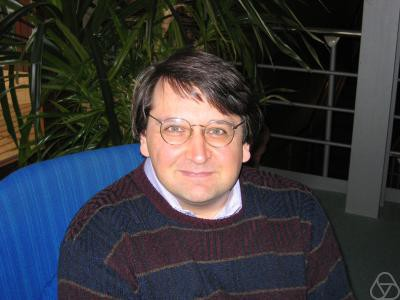
\includegraphics[height=0.30\textheight]{ch6_shephard_2004.jpg}\\[1mm]
\imgcap{Neil Shephard, 2004}
\imgcredit{https://commons.wikimedia.org/wiki/File:Shephard,_Neil_(1964).jpeg}{Photo: Renate Schmid (2004), MFO; CC BY-SA 2.0 de; Wikimedia Commons}
\end{column}
\begin{column}{0.68\textwidth}
\begin{itemize}
    \item $y_t = \exp(h_t/2)\,\epsilon_t$, $\quad h_{t+1} = \mu + \phi(h_t - \mu) + \sigma_\eta\eta_t$, $\quad \epsilon_t, \eta_t \sim$ i.i.d. $N(0, 1)$ \refTay
    \item $h_t$: log-variance, a latent AR(1) state; $\phi$: persistence; $\sigma_\eta$: volatility of volatility; $\exp(\mu/2)$: typical volatility
    \item A state space model with a nonlinear measurement equation: the Kalman filter does not apply directly
    \item Continuous-time counterpart: the log-variance as an Ornstein--Uhlenbeck process (option pricing, realised measures in \atschlink{https://danpele.github.io/Advanced-Time-Series/EN/Courses/chapter8_advanced_volatility.pdf}{Chapter 8})
\end{itemize}
\end{column}
\end{columns}
\end{frame}

\begin{frame}{Stochastic volatility is not GARCH}
\itemsize{\small}
\begin{itemize}
    \item GARCH \refBol: $\sigma^2_t = \omega + \alpha y^2_{t-1} + \beta\sigma^2_{t-1}$ ($\omega > 0$, $\alpha, \beta \ge 0$) is known at $t-1$ (measurable with respect to past returns): one source of randomness
    \begin{itemize}
        \item the likelihood is a product of known densities: one pass, exact ML
    \end{itemize}
    \item SV: $h_t$ has its own shock $\eta_t$; even with all past returns, today's variance is uncertain
    \begin{itemize}
        \item $p(y_{1:n} | \psi) = \int\prod_t N(y_t; 0, e^{h_t})\,p(h_{1:n} | \psi)\,dh_{1:n}$: an $n$-dimensional integral without closed form
    \end{itemize}
    \item Moments, with $\sigma^2_h = \sigma^2_\eta/(1 - \phi^2)$ the unconditional variance of $h_t$
    \begin{itemize}
        \item kurtosis of $y_t$: $3\exp(\sigma^2_h) > 3$ even with Gaussian $\epsilon_t$: fat tails come from the random variance
        \item $\Corr(y^2_t, y^2_{t-k}) = (e^{\sigma^2_h\phi^k} - 1)/(3e^{\sigma^2_h} - 1)$: volatility clustering that decays with $\phi^k$
    \end{itemize}
    \item Leverage enters as $\Corr(\epsilon_t, \eta_t) = \rho < 0$ \refOCSN; GARCH needs an asymmetric term for the same effect
    \item Comparison on the likelihood scale is possible only after the integral is computed: particle filter (next section) or importance sampling \refKSC
\end{itemize}
\end{frame}

\begin{frame}{A linear state space form: log-squared returns}
\itemsize{\small}
\begin{itemize}
    \item $y^*_t = \ln y^2_t = h_t + \xi_t$, $\xi_t = \ln\epsilon^2_t$: linear in $h_t$, but $\xi_t$ follows a $\ln\chi^2_1$ law with mean $-1.2704$ and variance $\pi^2/2 \approx 4.93$
    \item QML \refHRS: run the Kalman filter as if $\xi_t$ were $N(-1.2704, \pi^2/2)$; consistent, but inefficient
    \begin{itemize}
        \item $y^*_t$ is ARMA(1,1): $\Corr(y^*_t, y^*_{t-k}) = \phi^k\sigma^2_h/(\sigma^2_h + \pi^2/2)$, small because the noise dominates the signal
    \end{itemize}
    \item Zero returns: $\ln 0 = -\infty$; use $y^*_t = \ln(y^2_t + c)$ with a small offset $c$ (here $c = 10^{-3}\Var(y)$, scaled to the series)
    \item Multivariate extension of the same idea: factor SV models \refHRS
\end{itemize}
\end{frame}

\begin{frame}{The KSC mixture: a conditionally Gaussian model}
\itemsize{\footnotesize}
\begin{columns}[T]
\begin{column}{0.55\textwidth}
\begin{itemize}
    \item \refKSC: approximate $\ln\chi^2_1$ by a mixture of seven normals; given the component $s_t$, the model is linear and Gaussian
    \item $y^*_t = h_t + m_{s_t} - 1.2704 + \sqrt{v_{s_t}}\,u_t$, $u_t \sim N(0, 1)$, $P(s_t = i) = p_i$; $s_t \in \{1, \dots, 7\}$: the component; $p_i$, $m_i$, $v_i$: its probability, mean and variance (table)
    \item Mixture mean \ensuremath{-}1.2704 and variance 4.935, against $-1.2704$ and 4.935 for the exact law
    \item The residual approximation error can be removed by reweighting the draws (importance weights) \refKSC; finer 10-component mixtures \refOCSN
\end{itemize}
\end{column}
\begin{column}{0.42\textwidth}
\begin{center}
\scriptsize
\begin{tabular}{cccc}
\toprule
$i$ & $p_i$ & $m_i$ & $v_i$ \\
\midrule
1 & $0.00730$ & $-10.12999$ & $5.79596$ \\
2 & $0.10556$ & $-3.97281$ & $2.61369$ \\
3 & $0.00002$ & $-8.56686$ & $5.17950$ \\
4 & $0.04395$ & $2.77786$ & $0.16735$ \\
5 & $0.34001$ & $0.61942$ & $0.64009$ \\
6 & $0.24566$ & $1.79518$ & $0.34023$ \\
7 & $0.25750$ & $-1.08819$ & $1.26261$ \\
\bottomrule
\end{tabular}
\end{center}
\begin{itemize}
    \item Source: \refKSC, Table 4
\end{itemize}
\end{column}
\end{columns}
\end{frame}

\begin{frame}{The log chi-square law and its approximations}
\itemsize{\footnotesize}
\begin{center}
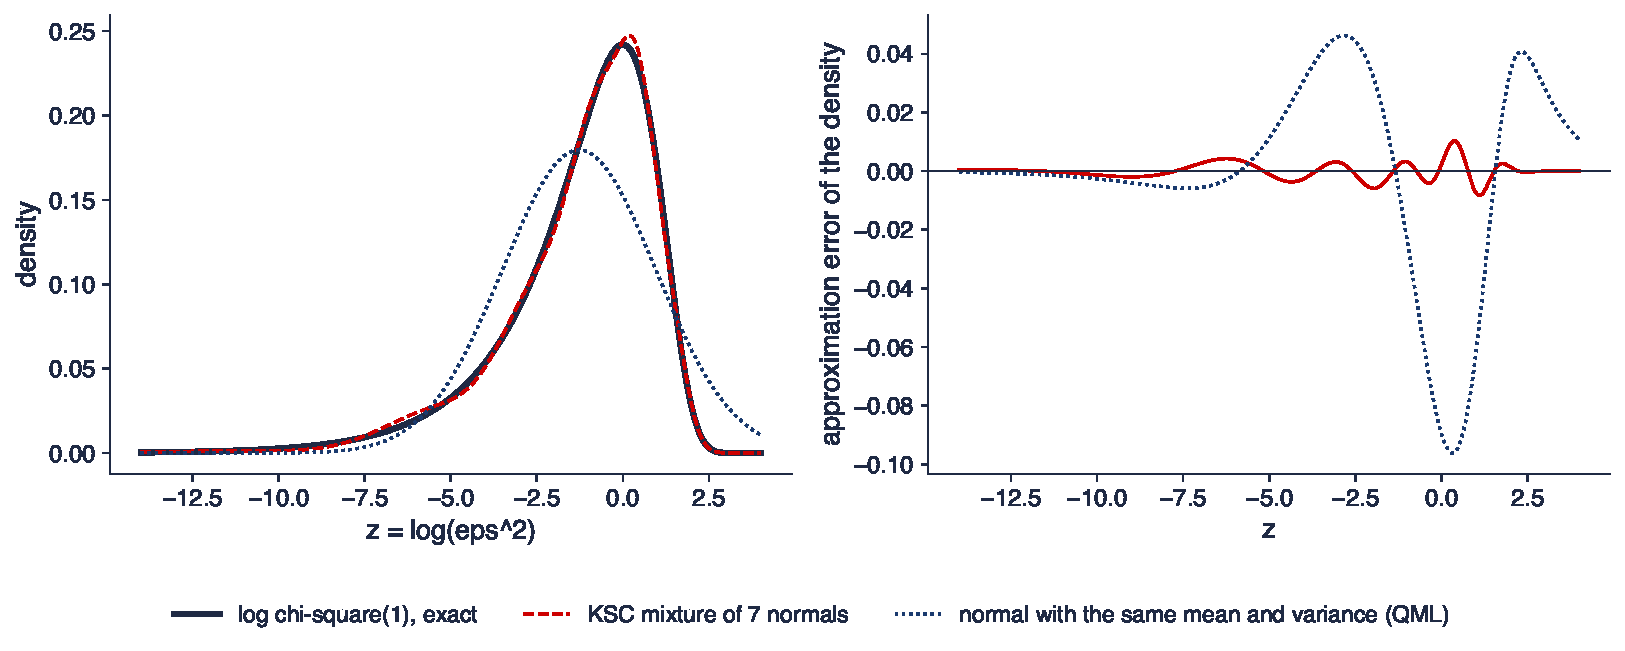
\includegraphics[width=0.97\textwidth,height=0.5\textheight,keepaspectratio]{ats_ch6_ksc.pdf}
\end{center}
\vspace{-0.25cm}
\begin{itemize}
    \item Left: density of $\ln\epsilon^2$ (exact), the KSC mixture and the normal with the same two moments used by QML; right: the two approximation errors
\end{itemize}
\quantlet{ATS\_ch6\_stochastic\_volatility}{\qlurl{ATS_ch6_stochastic_volatility}}
\end{frame}

\begin{frame}{Interpreting the mixture approximation}
\itemsize{\small}
\begin{itemize}
    \item The law is strongly skewed to the left: small returns produce very negative $\ln y^2_t$; the normal approximation misses both the skew and the peak
    \item Largest density error: 0.010 for the mixture, 0.096 for the normal (QML)
    \item QML treats a skewed noise as symmetric: the filter overreacts to near-zero returns; the mixture fixes this at the cost of one extra Gibbs block
\end{itemize}
\end{frame}

\begin{frame}{Gibbs sampling of the SV model}
\itemsize{\small}
\begin{itemize}
    \item Block 1: $s_t | y^*_t, h_t$ independently, $P(s_t = i) \propto p_i\,N(y^*_t - h_t;\ m_i - 1.2704, v_i)$
    \item Block 2: $h_{1:n} | s, \psi, y^*$ in one draw: a linear Gaussian model with known time-varying measurement variances $v_{s_t}$ (precision sampler or DK)
    \item Block 3: $\sigma^2_\eta | h, \mu, \phi$ inverse gamma; $\phi$ by Metropolis--Hastings with the AR(1) regression as proposal; $\mu$ normal
    \item Priors \refKSC: $(\phi + 1)/2 \sim \mathrm{Beta}(20, 1.5)$, $\sigma^2_\eta \sim IG(2.5, 0.025)$, $\mu \sim N(0, 10)$
    \item Single-move samplers (one $h_t$ at a time, \refJPR) mix very slowly because consecutive $h_t$ are highly correlated: sample the path as a block
\end{itemize}
\end{frame}

\begin{frame}{Stochastic volatility of the S\&P 500 and the BET}
\itemsize{\footnotesize}
\begin{center}
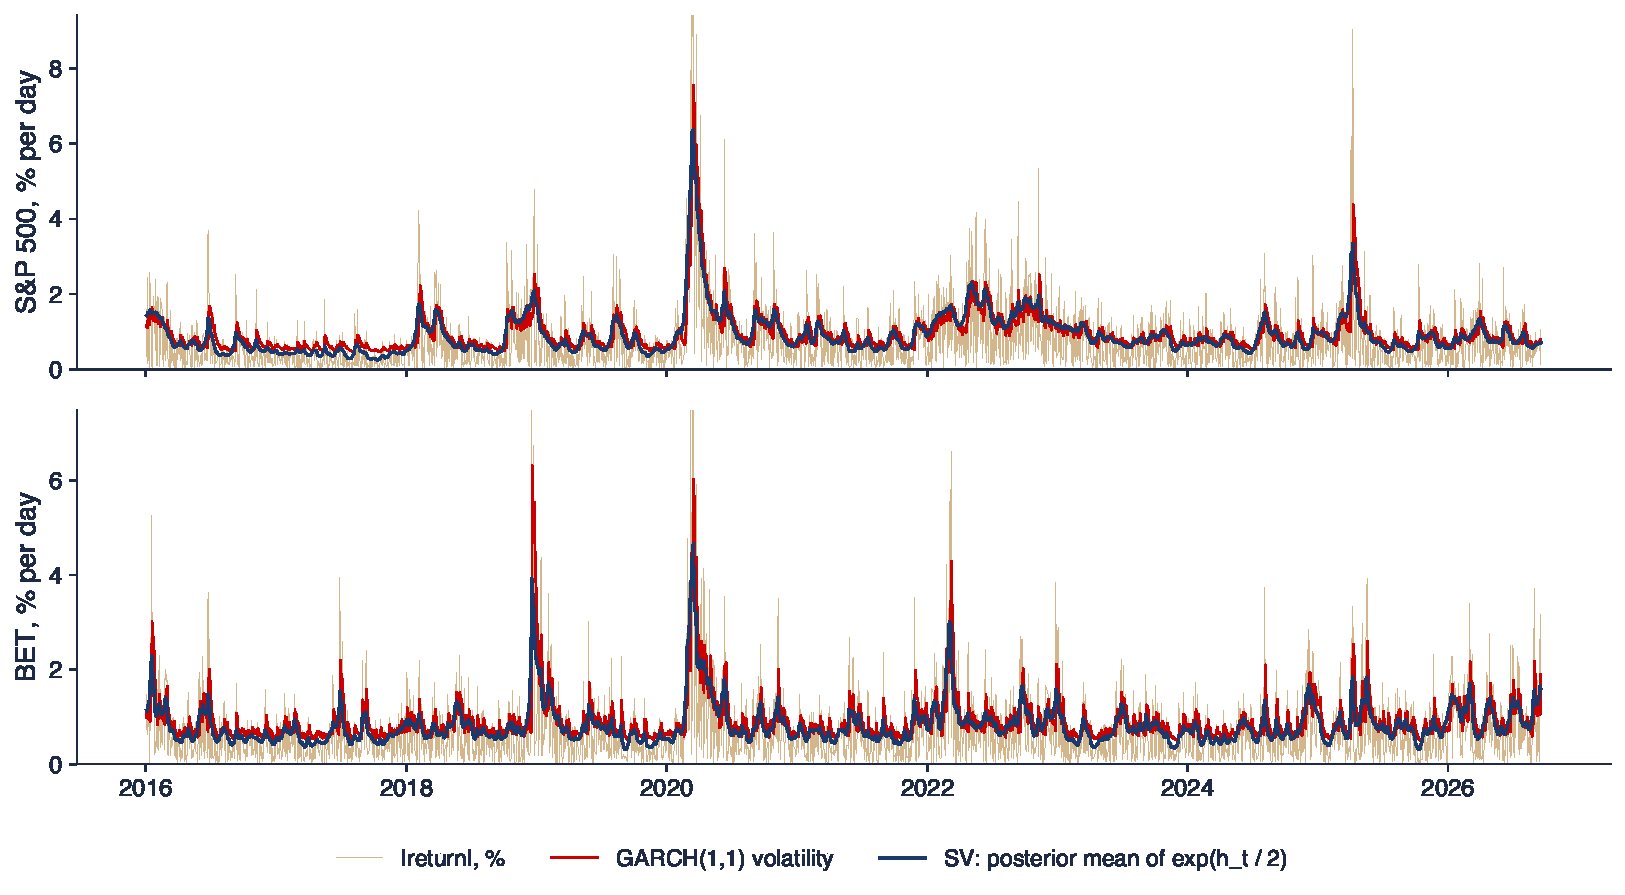
\includegraphics[width=0.97\textwidth,height=0.56\textheight,keepaspectratio]{ats_ch6_sv.pdf}
\end{center}
\vspace{-0.25cm}
\begin{itemize}
    \item Daily log returns in \%, demeaned, 2016--2026 ($T = 2692$ and 2675); KSC Gibbs sampler, 20\,000 draws; GARCH(1,1) by ML on the same data
\end{itemize}
\quantlet{ATS\_ch6\_stochastic\_volatility}{\qlurl{ATS_ch6_stochastic_volatility}}
\end{frame}

\begin{frame}{Interpreting the SV estimates}
\itemsize{\footnotesize}
\begin{center}
\footnotesize
\begin{tabular}{lcccccc}
\toprule
Index & $\phi$ & $\sigma_\eta$ & $\mu$ & ineff. $\phi$, $\sigma_\eta$ & GARCH $\alpha + \beta$ & corr. vol. \\
\midrule
S\&P 500 & 0.963 & 0.289 & \ensuremath{-}0.465 & 49 / 98 & 0.967 & 0.91 \\
BET & 0.914 & 0.393 & \ensuremath{-}0.624 & 58 / 87 & 0.952 & 0.84 \\
\bottomrule
\end{tabular}
\end{center}
\begin{itemize}
    \item 90\% intervals for $\phi$: [0.950; 0.975] (S\&P 500), [0.888; 0.938] (BET): very persistent log-variance, as in \refKSC
    \item The two volatility paths are close (correlation in the last column), but SV reacts less to a single large return than GARCH, whose variance jumps by $\alpha y^2_{t-1}$
    \item Large inefficiency factors for $\sigma_\eta$ are typical: $\sigma_\eta$ and the path $h_{1:n}$ are strongly dependent; long chains or interweaving are needed
    \item Kurtosis of returns: 19.5 (S\&P 500) and 20.8 (BET); with Gaussian $\epsilon_t$, SV explains only part of it (SV-$t$ errors are the usual extension)
\end{itemize}
\end{frame}

\begin{frame}{Recap: Stochastic volatility}
\itemsize{\small}
\begin{itemize}
    \item SV adds a shock to the variance: its likelihood is an integral over the volatility path
    \item Log-squared returns make the model linear; the KSC mixture makes it conditionally Gaussian, so the whole path can be drawn in one block
    \item On daily index returns SV and GARCH give similar volatility paths but different reactions to single large returns
\end{itemize}
\end{frame}


%=============================================================================
\section{Nonlinear and non-Gaussian filtering}
%=============================================================================

\begin{frame}{The Bayes filter}
\itemsize{\small}
\begin{itemize}
    \item General model: $y_t \sim g(y_t | x_t, \psi)$, $x_t \sim f(x_t | x_{t-1}, \psi)$; $g$: measurement density, $f$: transition density, $x_t$: the state; target $p(x_t | Y_t)$ and $p(y_t | Y_{t-1})$
    \item Prediction: $p(x_t | Y_{t-1}) = \int f(x_t | x_{t-1})\,p(x_{t-1} | Y_{t-1})\,dx_{t-1}$
    \item Update: $p(x_t | Y_t) = g(y_t | x_t)\,p(x_t | Y_{t-1}) / p(y_t | Y_{t-1})$, $\quad p(y_t | Y_{t-1}) = \int g(y_t | x_t)\,p(x_t | Y_{t-1})\,dx_t$
    \item Closed form only in two cases: linear Gaussian (Kalman) and finite state spaces (the Hamilton filter of Markov switching, \atschlink{https://danpele.github.io/Advanced-Time-Series/EN/Courses/chapter7_regime_switching_models.pdf}{Chapter 7})
    \begin{itemize}
        \item otherwise: approximate the model (EKF), approximate the densities by points (UKF), or by weighted samples (particle filters)
    \end{itemize}
\end{itemize}
\end{frame}

\begin{frame}{The extended Kalman filter}
\itemsize{\small}
\begin{itemize}
    \item Nonlinear model $y_t = Z(x_t) + \varepsilon_t$, $x_{t+1} = T(x_t) + R\eta_t$: linearise around the current estimates, $\dot Z_t = \partial Z/\partial x\,|_{a_t}$, $\dot T_t = \partial T/\partial x\,|_{a_{t|t}}$
    \item Run the Kalman recursions with $\dot Z_t, \dot T_t$ for the variances and the exact functions for the means \refDK, Section 10.2
    \item A failure that teaches: in SV, $\E(y_t | h_t) = 0$ for every $h_t$, so $\partial\E(y_t | h_t)/\partial h_t = 0$: the EKF gain is zero and the filter never learns $h_t$
    \begin{itemize}
        \item the information about $h_t$ is in $y^2_t$, a second moment; linearisation keeps only first moments
    \end{itemize}
    \item Rule: transform the model first ($\ln y^2_t$), or use a method that propagates the whole distribution
\end{itemize}
\end{frame}

\begin{frame}{The unscented Kalman filter}
\itemsize{\small}
\begin{itemize}
    \item Unscented transform \refJU: represent $N(m, P)$ ($n$ dimensions) by $2n + 1$ sigma points $\mathcal X_0 = m$, $\mathcal X_{\pm i} = m \pm (\sqrt{(n + \lambda)P})_i$
    \item Weights $w_0 = \lambda/(n + \lambda)$, $w_{\pm i} = 1/(2(n + \lambda))$; push each point through $g$ and take weighted means and covariances; $\lambda$: a spread parameter, $(\sqrt{A})_i$: the $i$-th column of a matrix square root
    \item Exact for the mean to second order of the Taylor expansion of $g$ (the EKF: first order); no Jacobians needed
    \item UKF: apply the transform in the prediction and in the update step; cost similar to the EKF
    \item Still Gaussian at each step: multimodal or heavy-tailed filtering densities need particles
\end{itemize}
\end{frame}

\begin{frame}{Linearisation against the unscented transform}
\itemsize{\footnotesize}
\begin{center}
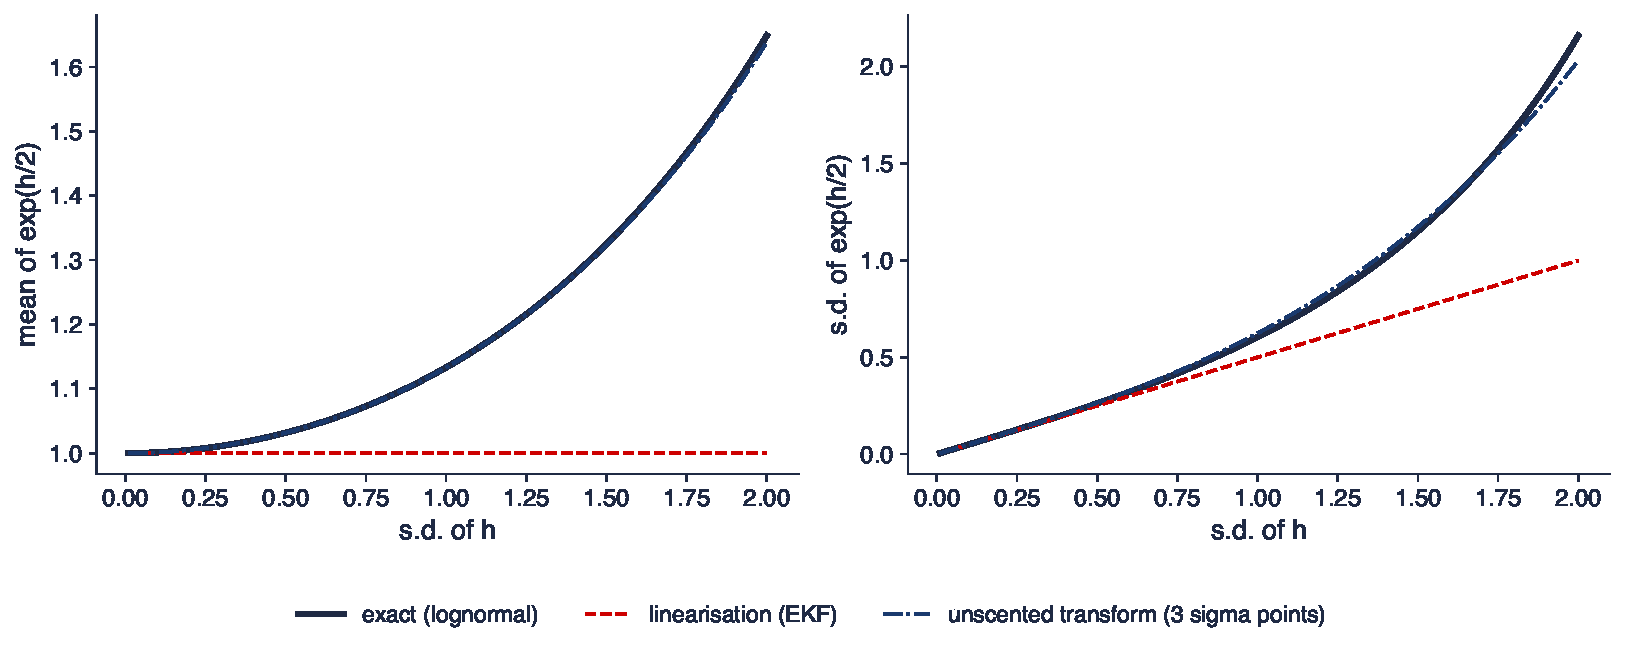
\includegraphics[width=0.97\textwidth,height=0.5\textheight,keepaspectratio]{ats_ch6_ukf.pdf}
\end{center}
\vspace{-0.25cm}
\begin{itemize}
    \item Volatility from log-variance: mean and s.d. of $\exp(h/2)$ for $h \sim N(0, s^2)$; exact lognormal moments, first-order linearisation (EKF) and the unscented transform with three sigma points
\end{itemize}
\quantlet{ATS\_ch6\_nonlinear\_filters}{\qlurl{ATS_ch6_nonlinear_filters}}
\end{frame}

\begin{frame}{Interpreting the unscented transform}
\itemsize{\small}
\begin{itemize}
    \item At $s = 1$: exact mean 1.131, linearisation 1.000, unscented 1.131; exact s.d. 0.598, linearisation 0.496, unscented 0.618
    \item Linearisation ignores the convexity of $\exp$: it underestimates expected volatility, more so when $h$ is uncertain
    \item Three sigma points capture the convexity almost exactly for the mean; the variance is off for large $s$
    \item Same bias in practice: an EKF forecast of volatility or of an option price is too low when the state is uncertain
\end{itemize}
\end{frame}

\begin{frame}{Particle filters}
\itemsize{\footnotesize}
\begin{columns}[T]
\begin{column}{0.3\textwidth}
\centering
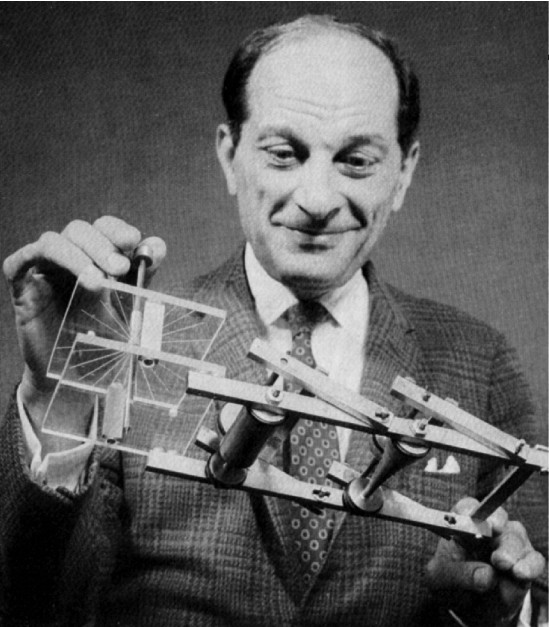
\includegraphics[height=0.32\textheight]{ch6_ulam_fermiac.jpg}\\[1mm]
\imgcap{Stanisław Ulam with the FERMIAC, a Monte Carlo device}
\imgcredit{https://commons.wikimedia.org/wiki/File:STAN_ULAM_HOLDING_THE_FERMIAC.jpg}{Photo: Los Alamos National Laboratory (LA-UR-00-2532); public domain; Wikimedia Commons}
\end{column}
\begin{column}{0.68\textwidth}
\begin{itemize}
    \item Represent $p(x_t | Y_t)$ by particles $x^{(i)}_t$ with weights $W^{(i)}_t$, $i = 1, \dots, N$; Monte Carlo goes back to Ulam and Metropolis (1949)
    \item Bootstrap filter \refGSS, \refKit: (1) propagate $x^{(i)}_t \sim f(\cdot | x^{(i)}_{t-1})$; (2) weight $w^{(i)}_t = g(y_t | x^{(i)}_t)$; (3) resample $N$ particles with probabilities $W^{(i)}_t \propto w^{(i)}_t$
    \item Without resampling the weights degenerate (one particle takes all the weight); effective sample size $\mathrm{ESS}_t = 1/\sum_i(W^{(i)}_t)^2$
    \item Systematic resampling: one uniform $U$, points $(U + i - 1)/N$ on the cumulative weights: lower variance than multinomial
\end{itemize}
\end{column}
\end{columns}
\end{frame}

\begin{frame}{The particle likelihood}
\itemsize{\small}
\begin{itemize}
    \item $\hat p(y_t | Y_{t-1}) = \frac1N\sum_i w^{(i)}_t$ and $\hat L(\psi) = \prod_t\hat p(y_t | Y_{t-1})$
    \item $\E\hat L(\psi) = L(\psi)$ exactly, for any $N \ge 1$ \refDM: unbiased on the level scale
    \begin{itemize}
        \item not on the log scale: if $\ln\hat L \approx N(\ln L - \tau^2/2, \tau^2)$, then $\E\ln\hat L = \ln L - \tau^2/2$; $\tau^2 = \Var\ln\hat L$
    \end{itemize}
    \item $\Var\ln\hat L$ grows roughly linearly in $n$ and falls like $1/N$: double the sample, double the particles
    \item $\hat L(\psi)$ is not smooth in $\psi$ (resampling is discontinuous): do not maximise it by gradient methods; use it inside MCMC
\end{itemize}
\end{frame}

\begin{frame}{Particle filter for the S\&P 500 SV model}
\itemsize{\footnotesize}
\begin{center}
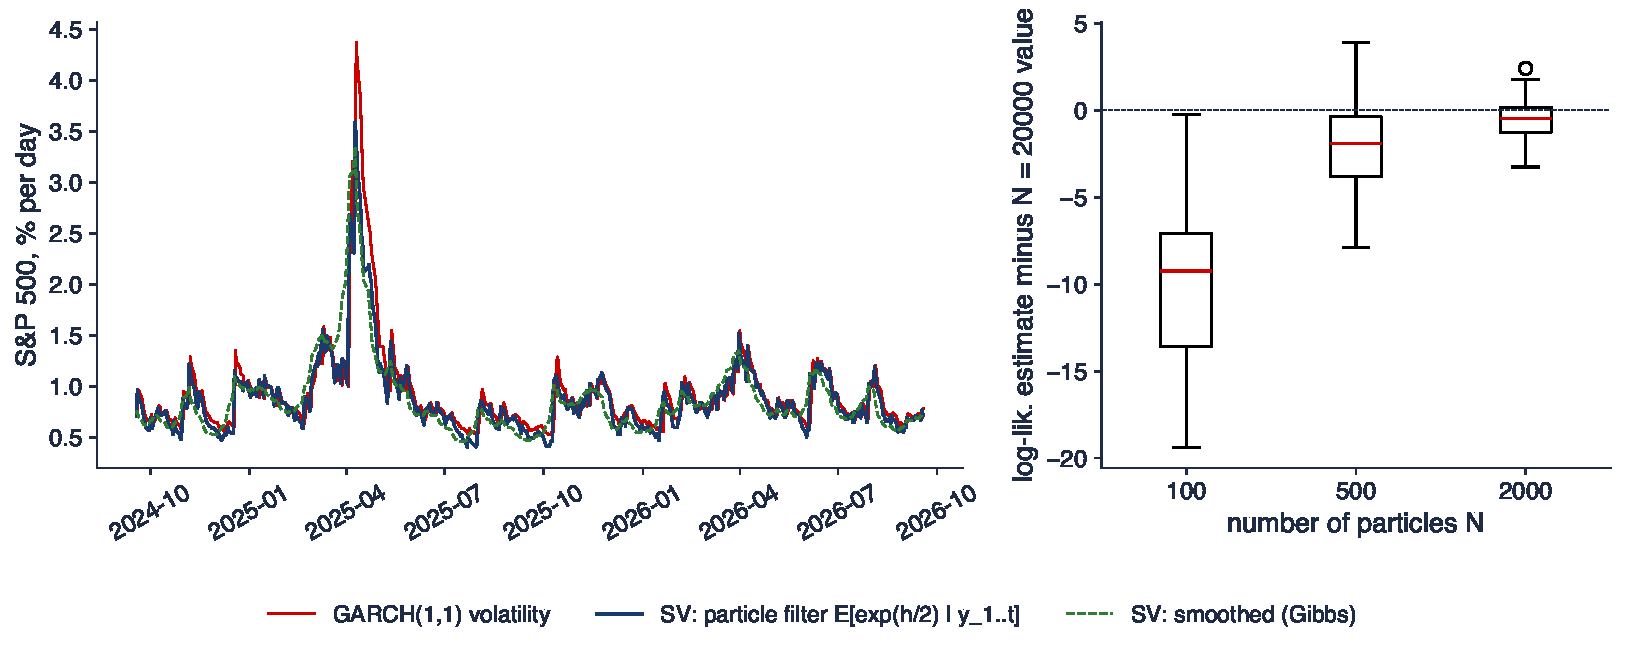
\includegraphics[width=0.97\textwidth,height=0.5\textheight,keepaspectratio]{ats_ch6_pf.pdf}
\end{center}
\vspace{-0.25cm}
\begin{itemize}
    \item Left: filtered volatility $\E[\exp(h_t/2) | Y_t]$ (bootstrap filter, $N = 20\,000$, Gibbs posterior mean of $\psi$) against GARCH(1,1) and the smoothed SV path, last two years; right: log-likelihood estimates, 100 runs per $N$
\end{itemize}
\quantlet{ATS\_ch6\_stochastic\_volatility}{\qlurl{ATS_ch6_stochastic_volatility}}
\end{frame}

\begin{frame}{Interpreting the particle filter}
\itemsize{\footnotesize}
\begin{itemize}
    \item Monte Carlo s.d. of $\ln\hat L$: 4.19 ($N = 100$), 2.38 ($N = 500$), 1.14 ($N = 2000$); small $N$ also biases $\ln\hat L$ downwards
    \item SV log-likelihood \ensuremath{-}3378.8 against the GARCH(1,1) maximum \ensuremath{-}3467.3: a difference of 88.5 with the same number of parameters
    \item The comparison favours SV even at the posterior mean (not the maximum) of its likelihood; \refKSC\ compare SV with ARCH models on the same likelihood scale
    \item The filtered SV volatility is a one-sided estimate, like GARCH: correlation 0.96; the smoothed path anticipates turning points because it uses future data
    \item Effective sample size over the sample: minimum 150, median 18719 of 20\,000 particles
\end{itemize}
\end{frame}

\begin{frame}{The auxiliary particle filter}
\itemsize{\small}
\begin{itemize}
    \item Bootstrap weakness: particles are propagated blind to $y_t$; an outlier leaves few particles with weight
    \item APF \refPS: look ahead before propagating. First stage: resample $x^{(i)}_{t-1}$ with weights $\propto W^{(i)}_{t-1}\,g(y_t | \mu^{(i)}_t)$, $\mu^{(i)}_t = \E(x_t | x^{(i)}_{t-1})$
    \begin{itemize}
        \item second stage: propagate, then weight by $g(y_t | x^{(i)}_t)/g(y_t | \mu^{(k_i)}_t)$ to correct the look-ahead
    \end{itemize}
    \item Fully adapted case: first-stage weights $p(y_t | x_{t-1})$ and proposal $p(x_t | x_{t-1}, y_t)$: second-stage weights are equal (locally optimal)
    \item The likelihood estimate stays unbiased: $\hat p(y_t | Y_{t-1}) = \big(\sum_iW^{(i)}_{t-1}g(y_t | \mu^{(i)}_t)\big)\cdot\frac1N\sum_i\omega^{(i)}_t$
\end{itemize}
\end{frame}

\begin{frame}{Particle likelihoods against the exact Kalman likelihood}
\itemsize{\footnotesize}
\begin{center}
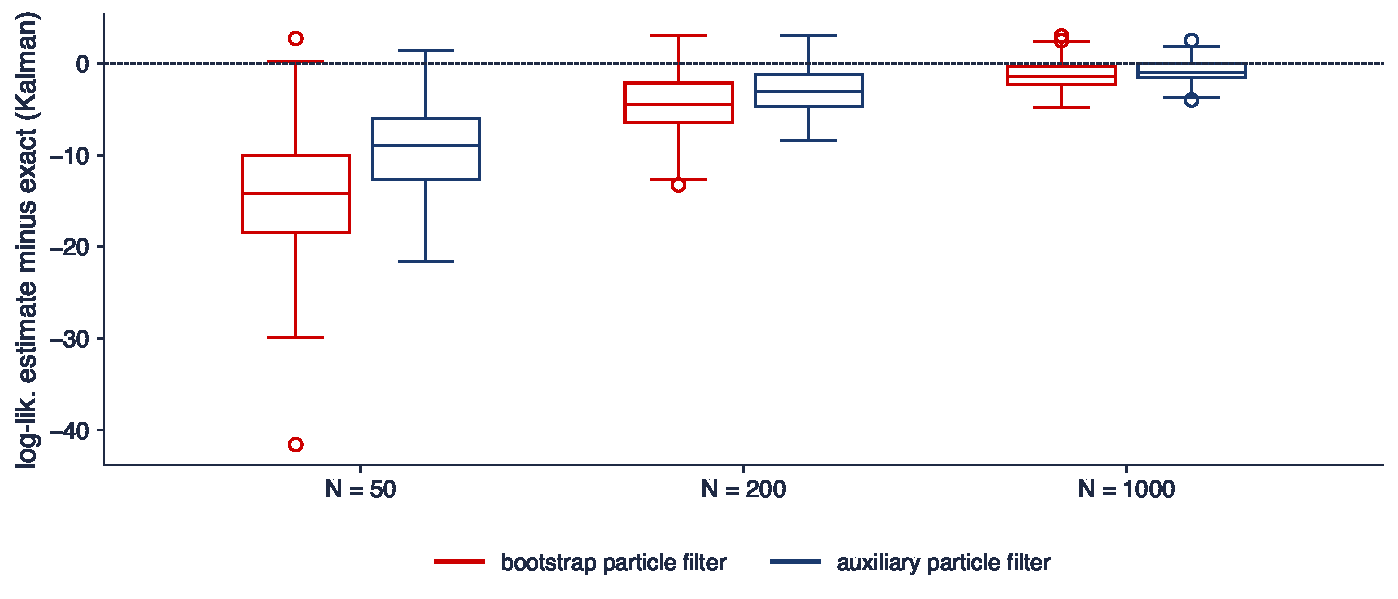
\includegraphics[width=0.97\textwidth,height=0.5\textheight,keepaspectratio]{ats_ch6_pf_check.pdf}
\end{center}
\vspace{-0.25cm}
\begin{itemize}
    \item Local level model for US inflation at the ML variances: error of $\ln\hat L$ (given $y_1$) for the bootstrap and the auxiliary filter, 200 runs per $N$
\end{itemize}
\quantlet{ATS\_ch6\_nonlinear\_filters}{\qlurl{ATS_ch6_nonlinear_filters}}
\end{frame}

\begin{frame}{Interpreting the particle check}
\itemsize{\small}
\begin{itemize}
    \item Mean error of $\ln\hat L$: \ensuremath{-}14.37, \ensuremath{-}4.48, \ensuremath{-}1.30 (bootstrap, $N = 50, 200, 1000$) and \ensuremath{-}9.37, \ensuremath{-}2.87, \ensuremath{-}0.88 (auxiliary)
    \item Standard deviations: 1.46 (bootstrap) and 1.17 (auxiliary) at $N = 1000$: the look-ahead buys precision because the signal-to-noise ratio is high
    \item The negative mean is the Jensen bias of a log of an unbiased estimator: it shrinks like $\Var(\ln\hat L)/2$
    \item Always test a particle filter on a model with a known likelihood before using it where none is available
\end{itemize}
\end{frame}

\begin{frame}{Particle MCMC}
\itemsize{\small}
\begin{itemize}
    \item Pseudo-marginal idea \refAR: run Metropolis--Hastings with an unbiased, positive estimate $\hat L(\psi)$ in place of $L(\psi)$; the chain still targets the exact posterior $p(\psi | Y_n)$
    \item PMMH \refADH: propose $\psi'$ from a proposal density $q(\cdot | \psi)$; run a particle filter for $\hat L(\psi')$; accept with probability $\min\{1, \hat L(\psi')p(\psi')q(\psi | \psi') / [\hat L(\psi)p(\psi)q(\psi' | \psi)]\}$; keep $\hat L$ of the current point
    \item Choosing $N$: too few particles make the chain stick; too many waste time. Target $\Var(\ln\hat L) \approx 1$--$2$ at the posterior mean \refPSGK, \refDPDK
    \begin{itemize}
        \item particle Gibbs (conditional SMC) samples the state path too; useful when no conditionally Gaussian structure exists
    \end{itemize}
    \item Works for any model you can simulate and whose measurement density you can evaluate: SV with jumps, DSGE models, nonlinear UC models
\end{itemize}
\end{frame}

\begin{frame}{PMMH against the KSC Gibbs sampler}
\itemsize{\footnotesize}
\begin{center}
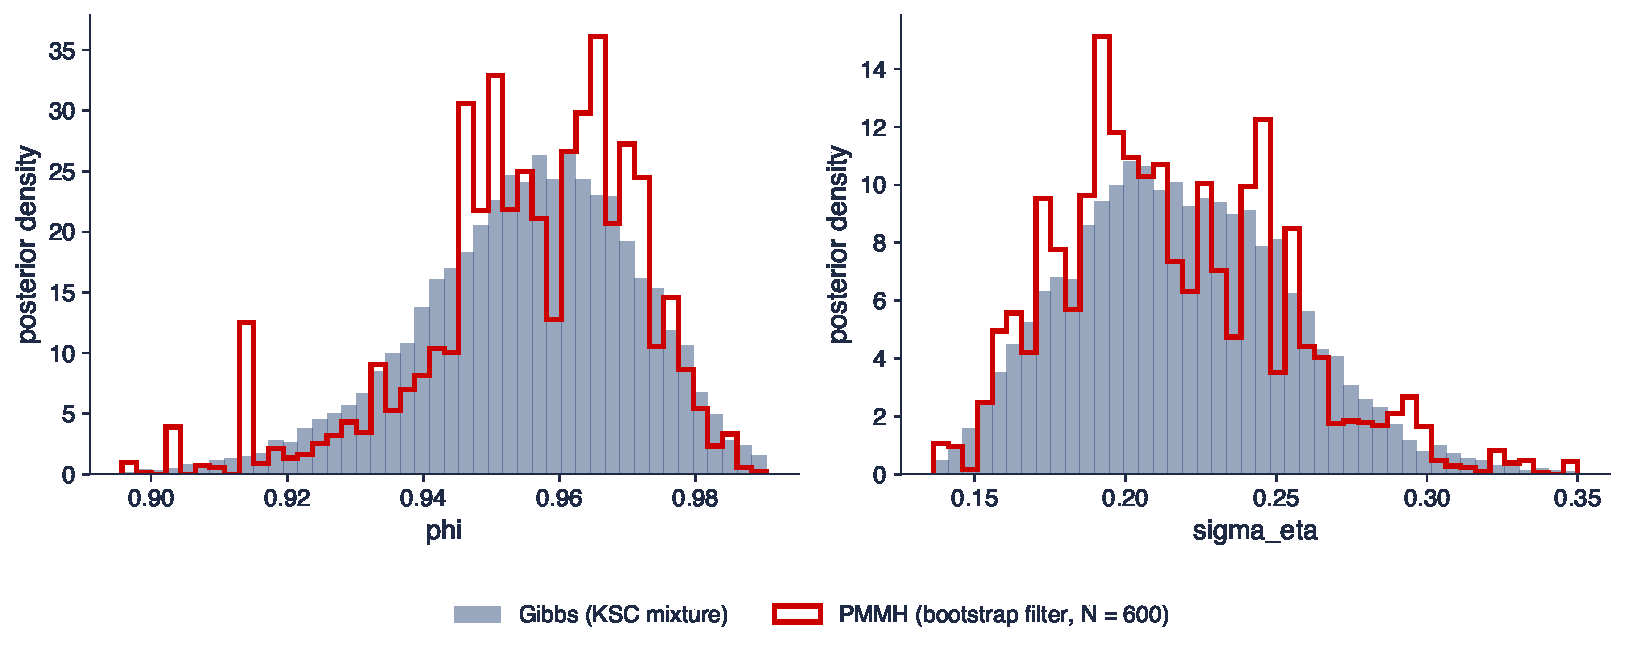
\includegraphics[width=0.97\textwidth,height=0.5\textheight,keepaspectratio]{ats_ch6_pmmh.pdf}
\end{center}
\vspace{-0.25cm}
\begin{itemize}
    \item Last 1000 S\&P 500 returns; PMMH with a bootstrap filter of $N = 600$ particles, 10\,000 iterations, random walk on $(\mu, \operatorname{atanh}\phi, \ln\sigma_\eta)$; Gibbs with the KSC mixture
\end{itemize}
\quantlet{ATS\_ch6\_stochastic\_volatility}{\qlurl{ATS_ch6_stochastic_volatility}}
\end{frame}

\begin{frame}{Interpreting the PMMH run}
\itemsize{\small}
\begin{itemize}
    \item Posterior means of $\phi$: 0.955 (Gibbs) and 0.955 (PMMH); of $\sigma_\eta$: 0.219 and 0.216; posterior s.d. 0.037 and 0.039
    \item Two exact algorithms, one posterior: the KSC mixture approximation has no visible effect here
    \item $N = 600$ gives s.d. of $\ln\hat L$ equal to 1.19 at the posterior mean, inside the recommended range; acceptance rate 13\%
    \item Cost: 3.6 minutes for PMMH against seconds for Gibbs: use PMMH when there is no conditionally Gaussian representation
\end{itemize}
\end{frame}

\begin{frame}{Recap: Nonlinear filtering}
\itemsize{\small}
\begin{itemize}
    \item EKF linearises the model, UKF propagates sigma points, particle filters propagate weighted samples
    \item The particle likelihood is unbiased in levels; its log variance decides the number of particles
    \item PMMH turns any simulable model into an exact Bayesian procedure, at a computational price
\end{itemize}
\end{frame}


%=============================================================================
\section{Time-varying parameters}
%=============================================================================

\begin{frame}{A TVP regression in state space form}
\itemsize{\small}
\begin{itemize}
    \item $y_t = c_t + b_tx_t + D_t'\gamma + \varepsilon_t$, $\quad c_{t+1} = c_t + \eta_{c,t}$, $\quad b_{t+1} = b_t + \eta_{b,t}$: state $\alpha_t = (c_t, b_t, \gamma')'$, $Z_t = (1, x_t, D_t')$; $c_t$, $b_t$: intercept and slope as random walks with variances $\sigma^2_c$, $\sigma^2_b$; $D_t$: dummies with fixed $\gamma$
    \item Fixed coefficients ($\gamma$, here quarterly seasonal dummies) are states with zero variance and a diffuse start: $d$ = number of states = 5
    \begin{itemize}
        \item with $\sigma^2_c = \sigma^2_b = 0$ the smoother returns the OLS estimates (recursive least squares)
    \end{itemize}
    \item Question: has the co-movement of Romanian inflation with euro-area inflation changed since inflation targeting began (2005)?
    \item $y_t$: Romanian HICP inflation, quarterly, \% a.r., not seasonally adjusted; $x_t$: euro-area HICP inflation net of its seasonal pattern; 2005Q4--2026Q2, $T = 83$
    \item Test of a constant slope: $H_0$: $\sigma^2_b = 0$ on the boundary; parametric bootstrap of the LR statistic from the restricted model (199 samples)
\end{itemize}
\end{frame}

\begin{frame}{Romanian on euro-area inflation: a time-varying slope?}
\itemsize{\footnotesize}
\begin{center}
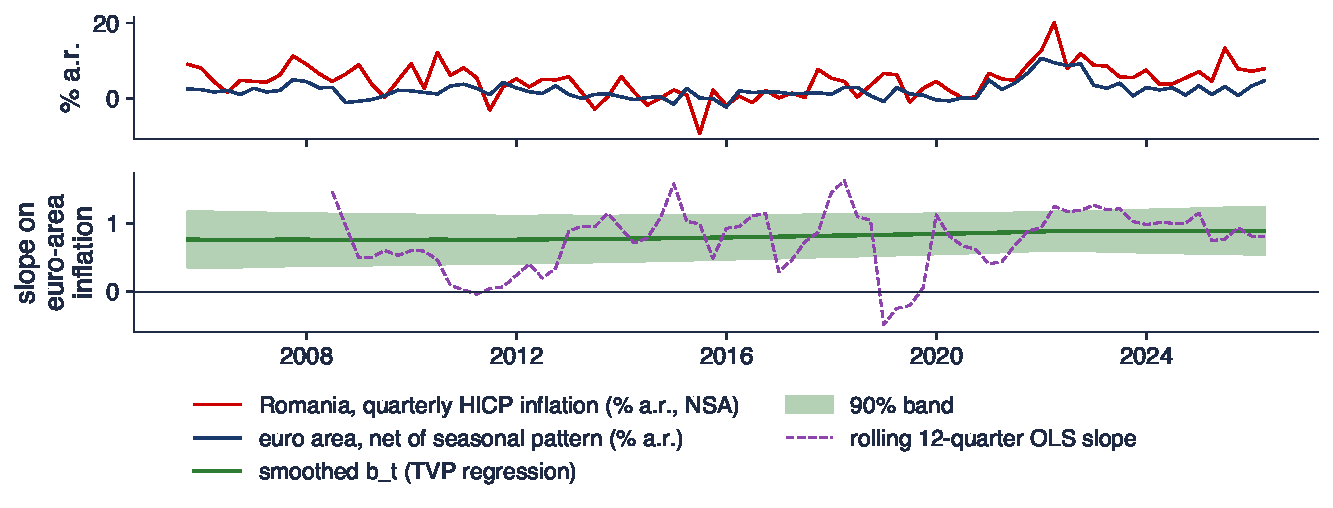
\includegraphics[width=0.97\textwidth,height=0.56\textheight,keepaspectratio]{ats_ch6_tvp.pdf}
\end{center}
\vspace{-0.25cm}
\begin{itemize}
    \item Top: the two inflation rates; bottom: smoothed $b_t$ with a 90\% band (exact diffuse ML) and the slope of a rolling 12-quarter regression with the same dummies
\end{itemize}
\quantlet{ATS\_ch6\_tvp\_inflation}{\qlurl{ATS_ch6_tvp_inflation}}
\end{frame}

\begin{frame}{Interpreting the TVP regression}
\itemsize{\small}
\begin{itemize}
    \item ML: $\hat\sigma^2_c = 0.332$, $\hat\sigma^2_b = 0.0011$, $\hat\sigma^2_\varepsilon = 7.21$; numpy and \texttt{statsmodels} log-likelihoods \ensuremath{-}209.93 and \ensuremath{-}209.93
    \item $b_t$ drifts from 0.76 (s.e. 0.23) in 2008Q3 to 0.89 (s.e. 0.17) in 2022Q4: a slope close to one, but no significant change
    \item LR $= 0.066$; bootstrap $p = 0.265$ (95\% quantile 1.91; 66\% of bootstrap statistics are exactly zero: pile-up again); the $\frac12\chi^2_1$ rule gives $p = 0.399$
    \item The rolling regression swings between negative values and 1.5: that is sampling noise of 12-quarter windows, not time variation; the state space model averages it out with an explicit variance
\end{itemize}
\end{frame}

\begin{frame}{TVP-VAR with stochastic volatility}
\itemsize{\footnotesize}
\begin{columns}[T]
\begin{column}{0.3\textwidth}
\centering
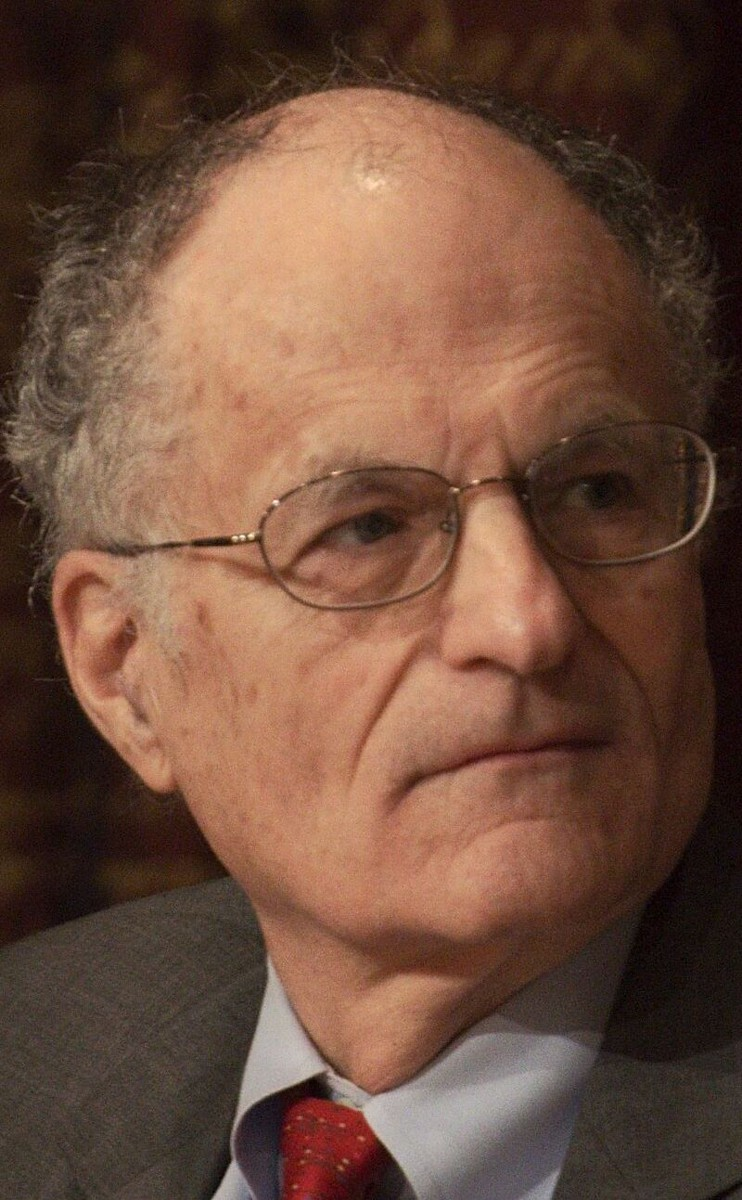
\includegraphics[height=0.36\textheight]{ch6_sargent_2011.jpg}\\[1mm]
\imgcap{Thomas J. Sargent, 2011}
\imgcredit{https://commons.wikimedia.org/wiki/File:Thomas_J._Sargent_close-up_(cropped).jpg}{Photo: Holger Motzkau (2011); CC BY-SA 3.0; Wikimedia Commons}
\end{column}
\begin{column}{0.68\textwidth}
\begin{itemize}
    \item \refCSa, \refCSb, \refPri: $y_t = X_t'\beta_t + A_t^{-1}\Sigma_t\epsilon_t$; $\beta_t$, the free elements $a_t$ of the lower-triangular $A_t$ and $\ln\sigma_{j,t}$ follow random walks; $X_t$: the lags; $\Sigma_t = \mathrm{diag}(\sigma_{j,t})$; $\epsilon_t \sim N(0, I)$
    \item Question: did US monetary policy change (drifting coefficients) or did the shocks shrink (falling volatilities) after 1980?
    \item Answer of \refPri: the systematic response of policy did change, but these changes explain little of the 1970s; the variance of non-policy shocks matters more
    \item Without stochastic volatility, falling shock variances are wrongly attributed to changing coefficients
\end{itemize}
\end{column}
\end{columns}
\end{frame}

\begin{frame}{Estimating a TVP-VAR-SV}
\itemsize{\small}
\begin{itemize}
    \item Gibbs blocks, each one of the samplers of this chapter:
    \begin{itemize}
        \item $\beta_{1:n}$ | rest: simulation smoother of a linear Gaussian model with known time-varying covariances
        \item $a_{1:n}$ | rest: equation by equation, the same smoother
        \item $\ln\sigma_{j,1:n}$ | rest: the KSC mixture with its indicators
        \item covariances of the random walks: inverse Wishart
    \end{itemize}
    \item The order of the Gibbs steps matters: the original algorithm drew the mixture indicators at the wrong point of the cycle; \refDNP\ give the corrected order, and the substantive results change little
    \item Priors from a training sample at the start of the data, as in \refPri, with small scales for the random-walk covariances: the prior decides how much variation is allowed
    \item Overparameterisation: with $k$ coefficients per equation, shrink the variances, or select which coefficients vary (non-centred parameterisation, \refFSW)
\end{itemize}
\end{frame}

\begin{frame}{Recap: Time-varying parameters}
\itemsize{\small}
\begin{itemize}
    \item A TVP regression is a state space model with $Z_t$ built from the regressors; fixed coefficients are diffuse states without shocks
    \item Rolling windows exaggerate time variation; test it at the boundary with a bootstrap
    \item TVP-VAR-SV combines the simulation smoother and the KSC mixture in one Gibbs sampler
\end{itemize}
\end{frame}


%=============================================================================
\section{Dynamic factor models in state space form}
%=============================================================================

\begin{frame}{The DFM as a state space model}
\itemsize{\small}
\begin{itemize}
    \item $x_{it} = \lambda_i'f_t + e_{it}$, $\quad f_t = \Phi f_{t-1} + u_t$, $\quad e_{it} = \rho_ie_{i,t-1} + \nu_{it}$: state $(f_t', f_{t-1}', e_t')'$, $Z = (\Lambda, 0, I)$
    \begin{itemize}
        \item $f_t$: the factors, a VAR(1) with matrix $\Phi$; $\lambda_i$: the loadings of series $i$, stacked in $\Lambda$; $e_{it}$: idiosyncratic AR(1) errors with coefficients $\rho_i$; $u_t$, $\nu_{it}$: shocks
    \end{itemize}
    \item Estimation:
    \begin{itemize}
        \item two steps \refDGR: principal components give $\Lambda$, $\Phi$, $\Sigma_e$; then the Kalman smoother re-estimates $f_t$ on the full panel; consistent as $N, T \to \infty$
        \item ML by EM \refSS, \refBM: the E-step is the smoother, arbitrary missing patterns are allowed
        \item large $N$: collapse the $N$ observations into an $r$-dimensional vector before filtering \refJK; the cost no longer grows with $N^3$
    \end{itemize}
    \item Mixed frequencies: a quarterly growth rate is a weighted sum of monthly states \refMM; missing months are simply skipped by the filter
    \item Nowcasting \refGRS: the ragged edge, news decomposition and real-time evaluation are in \atschlink{https://danpele.github.io/Advanced-Time-Series/EN/Courses/chapter5_bvar_factor_models_nowcasting.pdf}{Chapter 5}; this section shows the state space engine
\end{itemize}
\end{frame}

\begin{frame}{A one-factor model of the US coincident indicators}
\itemsize{\footnotesize}
\begin{center}
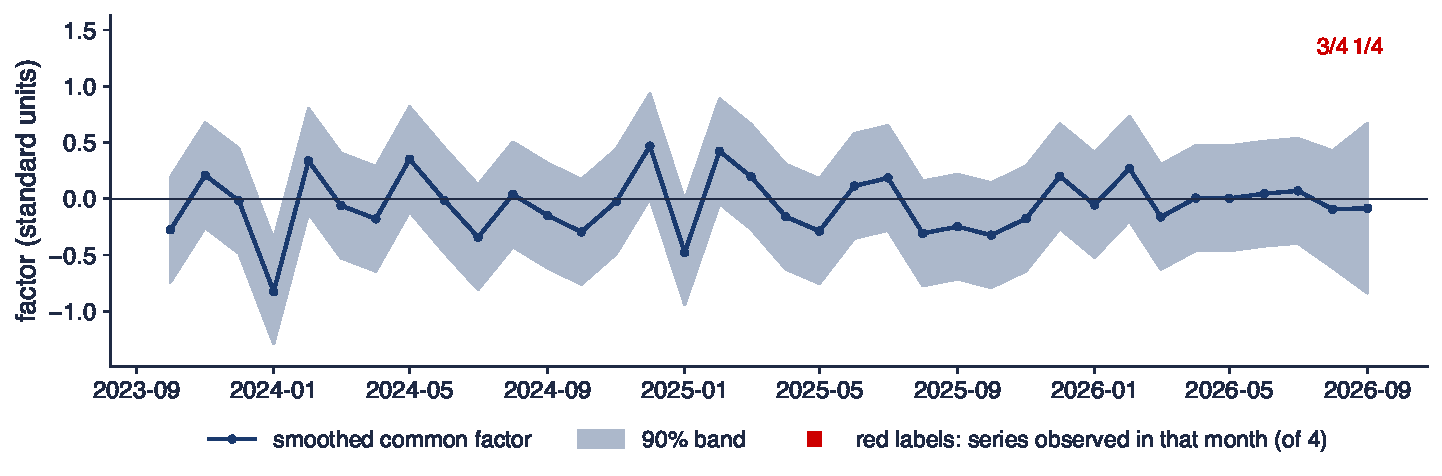
\includegraphics[width=0.97\textwidth,height=0.5\textheight,keepaspectratio]{ats_ch6_dfm.pdf}
\end{center}
\vspace{-0.25cm}
\begin{itemize}
    \item Monthly growth of industrial production, payrolls, real income less transfers and real sales (FRED), standardised, January 1990--September 2026; two-step estimator, univariate treatment of the observation vector; last 36 months
\end{itemize}
\quantlet{ATS\_ch6\_dfm\_ragged\_edge}{\qlurl{ATS_ch6_dfm_ragged_edge}}
\end{frame}

\begin{frame}{Interpreting the ragged edge}
\itemsize{\small}
\begin{itemize}
    \item Loadings 0.90, 0.89, 0.68, 0.84; factor AR coefficient 0.12: monthly growth rates have little persistence, so the factor is mostly a weighted average of the month
    \item The last complete month is July 2026: the factor s.d. is 0.28; in September 2026, with one series of four available, it rises to 0.46
    \item The filter weighs each series by its signal-to-noise ratio; no series is dropped, no gap is filled by hand
    \item Forecasting the factor beyond the data is the same recursion with all observations missing
\end{itemize}
\end{frame}


%=============================================================================
\section{Trend--cycle decompositions revisited}
%=============================================================================

\begin{frame}{Three definitions of the cycle}
\itemsize{\small}
\begin{itemize}
    \item Beveridge--Nelson \refBN: trend = long-horizon forecast net of drift, $\tau^{BN}_t = y_t + \sum_{j\ge1}\E_t(\Delta y_{t+j} - \mu)$; cycle $c^{BN}_t = y_t - \tau^{BN}_t$
    \begin{itemize}
        \item $\E_t$: expectation given data to $t$; $\mu$: mean growth; the trend is where $y$ is expected to settle once the predictable growth has died out
        \item for an AR(1) in growth: $c^{BN}_t = -\frac{\phi}{1 - \phi}(\Delta y_t - \mu)$; one-sided, depends on the ARMA chosen; reliable versions: \refKMW
    \end{itemize}
    \item Unobserved components \refCla, \refWat, \refHJ: $y_t = \tau_t + c_t$ with a random-walk (or smooth) trend and an AR(2) cycle; two-sided after smoothing
    \item Hamilton \refHamB: $c_{t+h}$ = residual of $y_{t+h}$ on $(1, y_t, \dots, y_{t-3})$, $h = 8$ quarters; model-free and one-sided (\atschlink{https://danpele.github.io/Time-Series-Analysis/EN/Courses/chapter10_state_space_kalman_markov_switching.pdf}{TSA, Chapter 10})
    \item For US GDP the BN cycle is small and noisy, the UC cycle large and smooth: the same data, two stories. Why?
\end{itemize}
\end{frame}

\begin{frame}{Unobserved components with correlated shocks}
\itemsize{\small}
\begin{itemize}
    \item \refMNZ: $y_t = \tau_t + c_t$, $\tau_t = \mu + \tau_{t-1} + \eta_t$, $c_t = \phi_1c_{t-1} + \phi_2c_{t-2} + \varepsilon_t$, $\Corr(\eta_t, \varepsilon_t) = \rho$ (UC-UR)
    \begin{itemize}
        \item $\tau_t$: the stochastic trend with drift $\mu$ and shocks $\eta_t$ (s.d. $\sigma_\eta$); $c_t$: an AR(2) cycle with shocks $\varepsilon_t$ (s.d. $\sigma_\varepsilon$); $\rho$: the correlation of the two shocks
    \end{itemize}
    \item Clark's UC0 imposes $\rho = 0$; with an AR(2) cycle, $\rho$ is identified: the reduced form is an ARIMA(2,1,2) with as many parameters as UC-UR
    \begin{itemize}
        \item with an AR(1) cycle, $\rho$ is not identified
    \end{itemize}
    \item Result: if $\rho$ is free, the filtered UC cycle equals the BN cycle of the ARIMA(2,1,2): the difference between BN and UC was the restriction $\rho = 0$
    \item State $(\tau_t, c_t, c_{t-1})$: $\tau$ diffuse, the cycle block stationary (mixed initialisation); case study below: their sample, 1947Q1--1998Q2, today's data vintage
\end{itemize}
\end{frame}

\begin{frame}{Replicating Morley, Nelson and Zivot (2003)}
\itemsize{\footnotesize}
\begin{center}
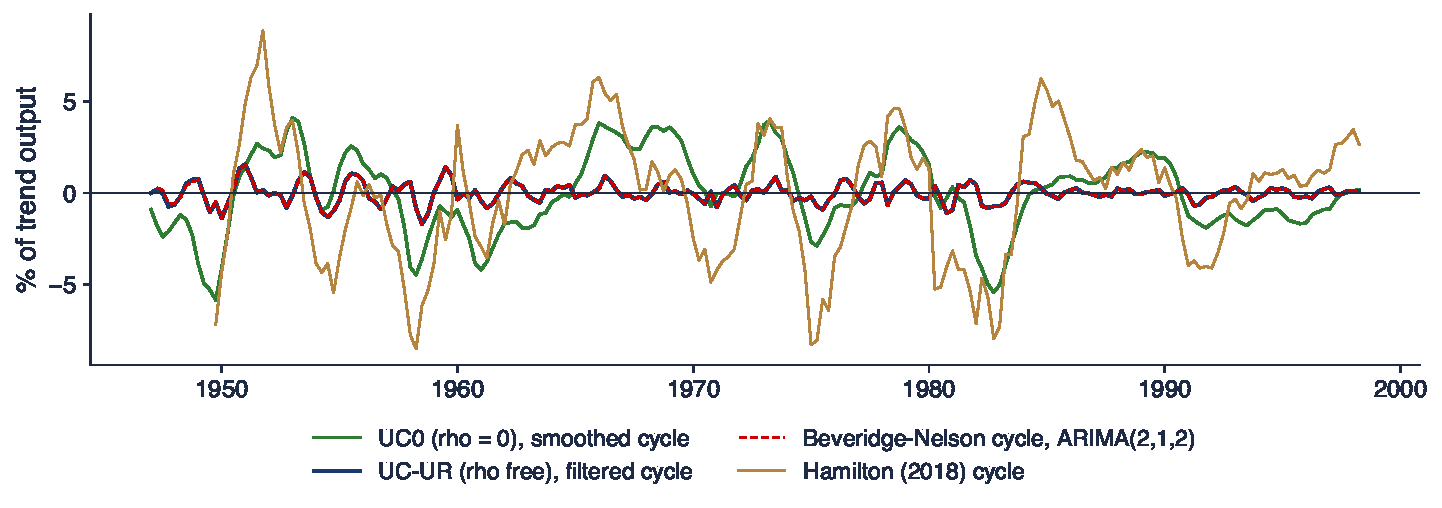
\includegraphics[width=0.97\textwidth,height=0.52\textheight,keepaspectratio]{ats_ch6_mnz.pdf}
\end{center}
\vspace{-0.25cm}
\begin{itemize}
    \item 100$\times$log US real GDP (FRED GDPC1), $T = 206$; UC0 and UC-UR by exact diffuse ML; BN cycle from an ARIMA(2,1,2); Hamilton (2018) cycle for comparison
\end{itemize}
\quantlet{ATS\_ch6\_trend\_cycle}{\qlurl{ATS_ch6_trend_cycle}}
\end{frame}

\begin{frame}{Interpreting the MNZ replication}
\itemsize{\footnotesize}
\begin{center}
\footnotesize
\begin{tabular}{lccccccc}
\toprule
Model & $\mu$ & $\phi_1$ & $\phi_2$ & $\sigma_\eta$ & $\sigma_\varepsilon$ & $\rho$ & $\ln L$ \\
\midrule
UC0 & 0.858 & 1.501 & \ensuremath{-}0.571 & 0.612 & 0.665 & 0 & \ensuremath{-}280.81 \\
UC-UR & 0.859 & 1.334 & \ensuremath{-}0.738 & 1.185 & 0.669 & \ensuremath{-}0.927 & \ensuremath{-}279.35 \\
\bottomrule
\end{tabular}
\end{center}
\begin{itemize}
    \item $\hat\rho = \ensuremath{-}0.927$: trend and cycle shocks are almost perfectly negatively correlated; trend shocks are larger than cycle shocks ($\hat\sigma_\eta > \hat\sigma_\varepsilon$)
    \item Correlation of the UC-UR filtered cycle with the BN cycle (ARIMA AR roots 1.334, \ensuremath{-}0.738 as in UC-UR): 0.999; s.d. of the cycles: UC0 2.20, UC-UR 0.52, BN 0.52, Hamilton 3.50
    \item LR test of $\rho = 0$: 2.92, $p = 0.088$ ($\chi^2_1$); the cycle of UC0 is large because it is assumed orthogonal to the trend, not because the data demand it
    \item Our numbers use today's GDP vintage; the paper's estimates differ in the decimals, not in the conclusion
\end{itemize}
\end{frame}

\begin{frame}{Romania: the cycle is the trend}
\itemsize{\footnotesize}
\begin{columns}[T]
\begin{column}{0.3\textwidth}
\centering
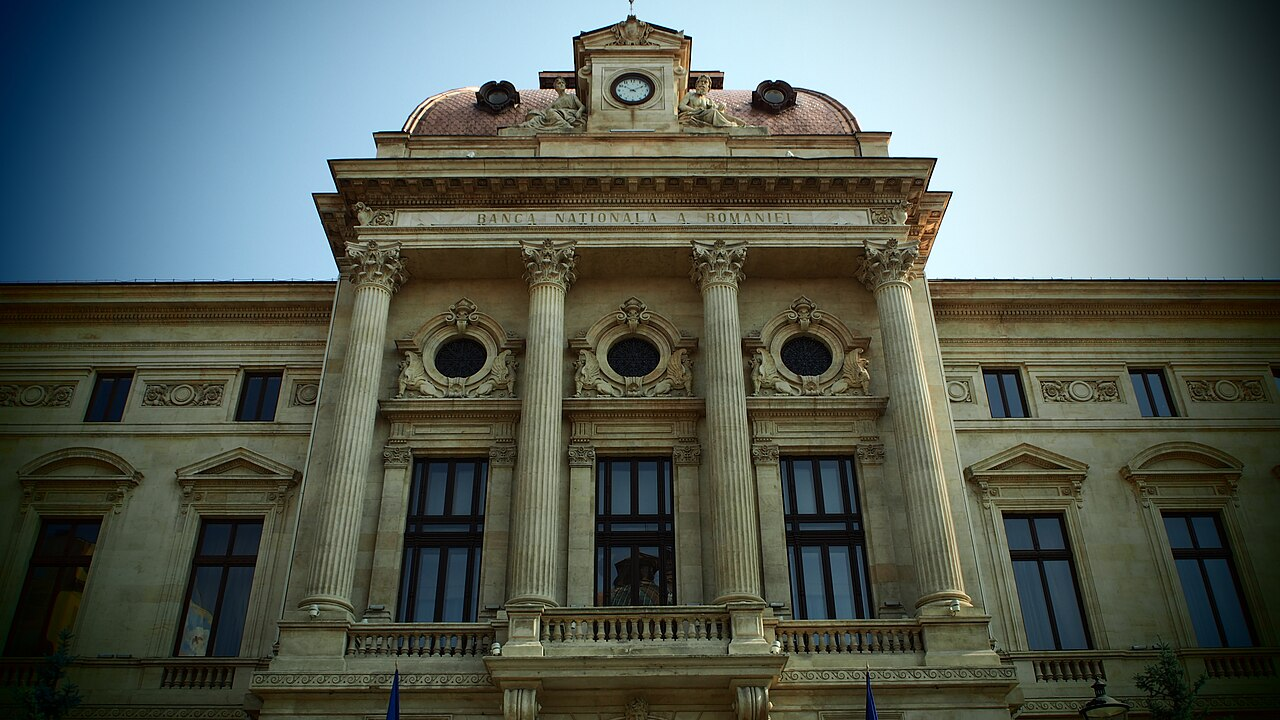
\includegraphics[height=0.30\textheight]{ch0_bnr_palace_2015.jpg}\\[1mm]
\imgcap{The BNR palace, Bucharest}
\imgcredit{https://commons.wikimedia.org/wiki/File:Bucharest_-_BNR_Palace_(19644434340).jpg}{Photo: Ștefan Jurcă (2015); CC BY 2.0; Wikimedia Commons}
\end{column}
\begin{column}{0.68\textwidth}
\begin{itemize}
    \item Emerging economies have volatile trend shocks \refAG: a random-walk trend absorbs most of the movement in GDP
    \item Romanian UC0, 2000Q1--2026Q2 (2020Q2--Q4 treated as missing): $\hat\sigma_\eta = 1.897$, $\hat\sigma_\varepsilon = 0.950$, $\hat\phi_1 = 0.280$, $\hat\phi_2 = \ensuremath{-}0.261$: a short, weak cycle
    \item UC-UR: $\hat\rho = 1.00$ at the boundary, LR $= 2.92$: in 106 quarters the correlation is poorly determined
    \item Alternative: a smooth trend (integrated random walk, the HP model \refHJ) with an AR(2) cycle: $\hat\sigma^2_\zeta = 0.0046$, $\hat\sigma^2_\varepsilon = 4.95$, $\hat\phi = (0.87, 0.09)$
\end{itemize}
\end{column}
\end{columns}
\end{frame}

\begin{frame}{The Romanian output gap}
\itemsize{\footnotesize}
\begin{center}
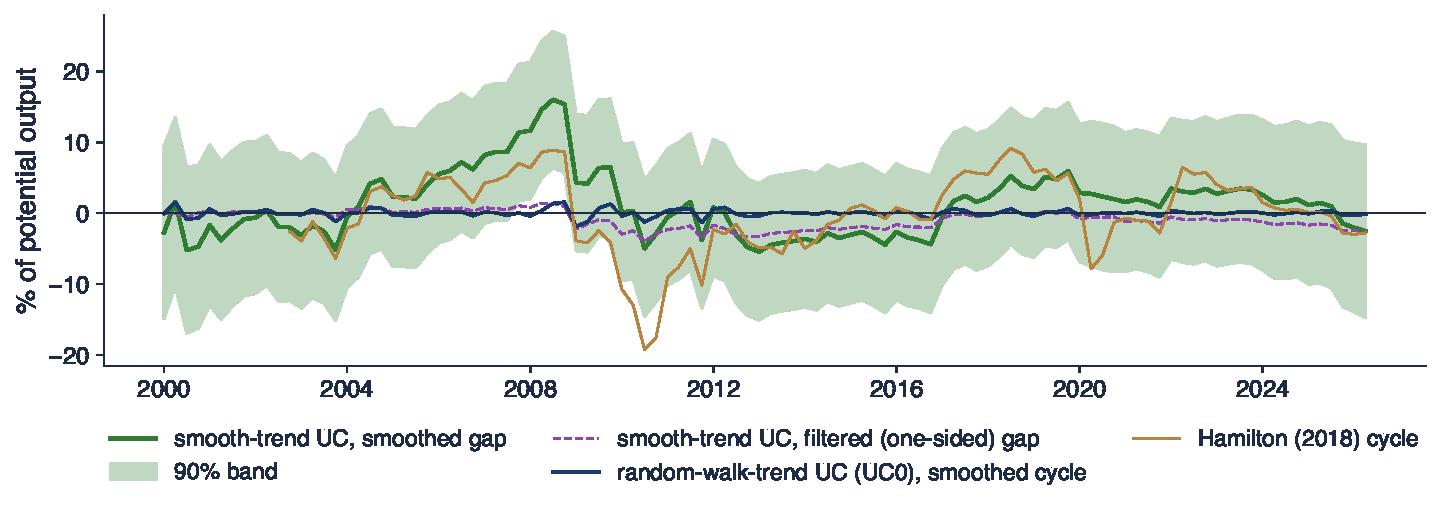
\includegraphics[width=0.97\textwidth,height=0.52\textheight,keepaspectratio]{ats_ch6_ro_gap.pdf}
\end{center}
\vspace{-0.25cm}
\begin{itemize}
    \item 100$\times$log real GDP, Eurostat, seasonally and calendar adjusted; smooth-trend UC (smoothed, with 90\% band, and filtered), random-walk-trend UC0, Hamilton (2018) on the full series
\end{itemize}
\quantlet{ATS\_ch6\_trend\_cycle}{\qlurl{ATS_ch6_trend_cycle}}
\end{frame}

\begin{frame}{Interpreting the Romanian output gap}
\itemsize{\small}
\begin{itemize}
    \item Smooth-trend gap: 16.0\% in 2008Q3 (s.d. 5.9), \ensuremath{-}5.0\% in 2010Q3, 5.9\% in 2019Q4; last quarter \ensuremath{-}2.6\% (s.d. 7.4)
    \item Real time is different: the filtered gap was only 1.4\% in 2008Q3 and 0.3\% in 2019Q4; s.d. of the revisions (smoothed minus filtered): 3.8 pp \refOvN
    \item Model choice dominates: s.d. of the gap 4.5 (smooth trend), 0.53 (UC0), 5.4 (Hamilton); correlation smooth trend--Hamilton 0.65
    \item A Romanian output gap without its band and without the model behind it is not information
\end{itemize}
\end{frame}

\begin{frame}{Recap: Trend--cycle decompositions}
\itemsize{\small}
\begin{itemize}
    \item BN, UC and Hamilton define the cycle differently; MNZ show that BN and UC agree once trend and cycle shocks may correlate
    \item In short, volatile samples (Romania) the correlation is not identified and the trend specification decides the gap
    \item Report filtered and smoothed estimates: the end-of-sample gap is the least reliable number
\end{itemize}
\end{frame}


%=============================================================================
\section{Trend inflation with stochastic volatility}
%=============================================================================

\begin{frame}{The UC-SV model of Stock and Watson (2007)}
\itemsize{\small}
\begin{itemize}
    \item $\pi_t = \tau_t + \sigma_{\eta,t}\eta_t$, $\quad \tau_t = \tau_{t-1} + \sigma_{\varepsilon,t}\varepsilon_t$, $\quad \ln\sigma^2_{j,t} = \ln\sigma^2_{j,t-1} + \nu_{j,t}$, $\nu_{j,t} \sim N(0, \gamma)$ \refSWb
    \begin{itemize}
        \item $\pi_t$: inflation; $\tau_t$: trend inflation (a random walk); $\sigma_{\eta,t}$, $\sigma_{\varepsilon,t}$: the time-varying s.d. of the transitory and trend shocks ($j \in \{\eta, \varepsilon\}$); $\eta_t, \varepsilon_t \sim N(0, 1)$
    \end{itemize}
    \item $\gamma = 0.2$ is fixed, not estimated: the only tuning parameter; it governs how fast the volatilities can move
    \begin{itemize}
        \item reduced form: IMA(1,1) with a time-varying MA coefficient $\theta_t$, a function of $\sigma_{\varepsilon,t}/\sigma_{\eta,t}$
    \end{itemize}
    \item Gibbs: $\tau_{1:n}$ by the precision sampler (time-varying weights); each $\ln\sigma^2_{j,1:n}$ by the KSC mixture on $\ln(\hat\eta^2_t + c)$ and $\ln(\Delta\tau^2_t + c)$
    \begin{itemize}
        \item for Romania: three quarterly seasonal coefficients as an extra Gibbs block (weighted regression); the HICP is not seasonally adjusted
    \end{itemize}
    \item Why it matters: the share of trend shocks decides how much of an inflation surge is permanent and how much a forecaster should extrapolate
\end{itemize}
\end{frame}

\begin{frame}{US trend inflation, 1953--2026}
\itemsize{\footnotesize}
\begin{center}
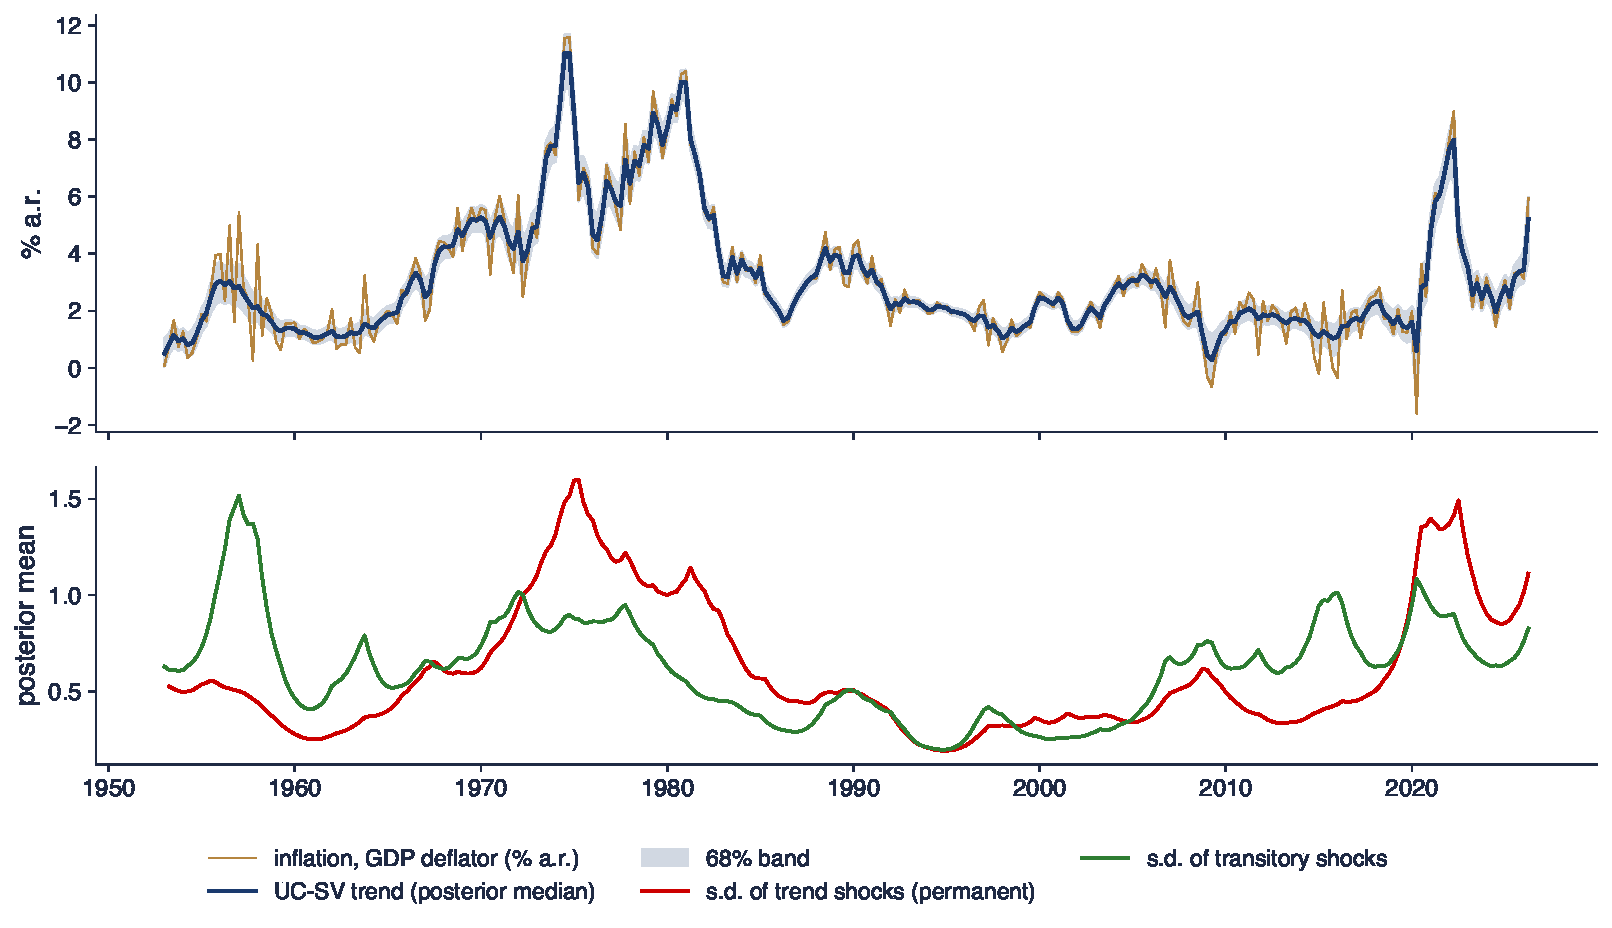
\includegraphics[width=0.97\textwidth,height=0.56\textheight,keepaspectratio]{ats_ch6_ucsv_us.pdf}
\end{center}
\vspace{-0.25cm}
\begin{itemize}
    \item GDP-deflator inflation, $T = 294$ quarters; UC-SV with $\gamma = 0.2$, Gibbs sampler; top: trend with 68\% band; bottom: posterior means of $\sigma_{\varepsilon,t}$ (trend) and $\sigma_{\eta,t}$ (transitory)
\end{itemize}
\quantlet{ATS\_ch6\_ucsv\_inflation}{\qlurl{ATS_ch6_ucsv_inflation}}
\end{frame}

\begin{frame}{Interpreting US trend inflation}
\itemsize{\footnotesize}
\begin{itemize}
    \item Trend: 8.9\% in 1975Q1, 2.1\% in 1995Q1, 1.4\% in 2019Q4, 8.0\% [6.6; 8.9] in 2022Q2, 5.2\% [3.8; 6.0] in 2026Q2
    \item Trend shocks: s.d. 1.60 in 1975, 0.19 in 1995, 1.42 in 2022; transitory shocks: 0.88, 0.20, 0.90
    \item Implied MA coefficient $\theta_t$: \ensuremath{-}0.20 (1975), \ensuremath{-}0.39 (1995), \ensuremath{-}0.37 (2019), \ensuremath{-}0.24 (2022): inflation became more like a random walk again in 2021--2022
    \item This is the forecasting lesson of \refSWb: in calm periods smooth heavily; when trend volatility rises, a fixed-coefficient model reacts too slowly
\end{itemize}
\end{frame}

\begin{frame}{Romanian trend inflation and the BNR target}
\itemsize{\footnotesize}
\begin{center}
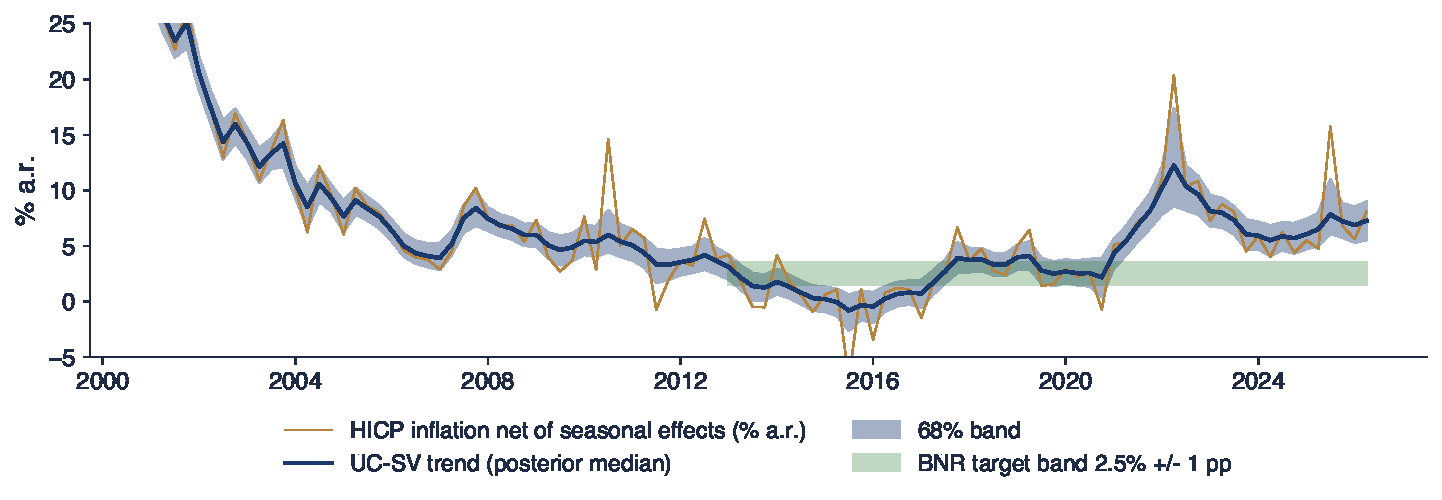
\includegraphics[width=0.97\textwidth,height=0.52\textheight,keepaspectratio]{ats_ch6_ucsv_ro.pdf}
\end{center}
\vspace{-0.25cm}
\begin{itemize}
    \item Quarterly HICP inflation (quarterly averages of the monthly index), $T = 102$, 2001Q1--2026Q2; UC-SV with $\gamma = 0.2$ and quarterly seasonal dummies; inflation-target band of the BNR since 2013
\end{itemize}
\quantlet{ATS\_ch6\_ucsv\_inflation}{\qlurl{ATS_ch6_ucsv_inflation}}
\end{frame}

\begin{frame}{Interpreting Romanian trend inflation}
\itemsize{\small}
\begin{itemize}
    \item Trend: 8.4\% when inflation targeting began (2005Q3), \ensuremath{-}0.8\% in 2015Q3, 2.5\% in 2019Q4, 8.1\% in 2023Q1
    \item Last quarter: 7.3\% [5.5; 9.0]; posterior probability that the trend lies inside 1.5--3.5\%: 2\%
    \item Since 2013 the trend has been inside the band only part of the time: below it in 2015--2016 (VAT cuts), above it since 2021
    \item Caveats: administered prices (energy caps, VAT changes) enter as trend shocks in a univariate model; a project can add them as regressors or as a separate component
\end{itemize}
\end{frame}

\begin{frame}{Beyond: BSTS and regime switching}
\itemsize{\small}
\begin{itemize}
    \item Bayesian structural time series \refSV: local linear trend + seasonal + regression with a spike-and-slab prior on many regressors (Google Trends)
    \begin{itemize}
        \item the same simulation smoother inside a Gibbs sampler; variable selection on the regression block
        \item counterfactuals for policy evaluation (CausalImpact, \refBro): \atschlink{https://danpele.github.io/Advanced-Time-Series/EN/Courses/chapter14_causal_inference_time_series.pdf}{Chapter 14}
    \end{itemize}
    \item Discrete states: $s_t \in \{1, \dots, K\}$ with a Markov chain; the Hamilton filter is the Bayes filter with sums instead of integrals
    \begin{itemize}
        \item state space models with regime switching (Kim filter, Gibbs sampling) \refKN: \atschlink{https://danpele.github.io/Advanced-Time-Series/EN/Courses/chapter7_regime_switching_models.pdf}{Chapter 7}
    \end{itemize}
    \item Forecast evaluation of all these models (density forecasts, scoring rules): \atschlink{https://danpele.github.io/Advanced-Time-Series/EN/Courses/chapter1_forecast_evaluation.pdf}{Chapter 1}
\end{itemize}
\end{frame}

\begin{frame}{Recap: Trend inflation}
\itemsize{\small}
\begin{itemize}
    \item UC-SV lets the split between permanent and transitory shocks change over time
    \item Two KSC blocks and one precision sampler make the Gibbs sampler fast
    \item US trend inflation rose sharply in 2021--2022; Romanian trend inflation is still above the target band
\end{itemize}
\end{frame}


%=============================================================================
\section{AI for scientific discovery}
%=============================================================================

\begin{frame}{An open question}
\itemsize{\small}
\begin{itemize}
    \item How much of the 2021--2023 inflation surge was a shift in trend inflation, in the US and in Romania, and has it been reversed?
    \begin{itemize}
        \item formal: the posterior of $\tau_t$ and of $\sigma_{\varepsilon,t}/\sigma_{\eta,t}$ in UC-SV; falsified if the trend has returned to its 2019 level with high posterior probability under every pre-registered specification
        \item the univariate answer depends on one fixed parameter, $\gamma$: the mini-case below
    \end{itemize}
    \item Why it matters: a central bank reacts differently to a transitory and to a persistent surge; anchoring is a statement about the trend, not about headline inflation
    \begin{itemize}
        \item literature to start from: \refSWb, \refCSb, \refPri, \refMNZ
    \end{itemize}
\end{itemize}
\end{frame}

\begin{frame}{The discovery loop with an AI assistant}
\itemsize{\footnotesize}
\begin{itemize}
    \item An AI assistant (an LLM such as Claude, ChatGPT, Gemini or Copilot) speeds up each step; Semantic Scholar and Elicit help with the literature
    \begin{itemize}
        \item \textbf{literature}: \aiprompt{List peer-reviewed papers that estimate trend inflation with stochastic volatility for European countries after 2021; give DOIs.} Then check every DOI on Crossref
        \item \textbf{hypothesis}: \aiprompt{Propose three observable implications that distinguish a trend shift from a sequence of large transitory shocks.}
        \item \textbf{code and replication}: ask for a UC-SV Gibbs sampler, then reproduce a known number first (the US trend of this lecture)
        \item \textbf{robustness and critique}: \aiprompt{Act as a hostile referee: which fixed choices of a UC-SV model could change the conclusion about 2022?}
    \end{itemize}
    \item Report: what was asked, what was kept, what was rejected (AI\_USE.md, AI\_ERRORS.md)
\end{itemize}
\end{frame}

\begin{frame}{What the human checks}
\itemsize{\small}
\begin{itemize}
    \item Every reference exists and says what is claimed (DOI resolves, title matches, the result is in the paper)
    \item The sampler targets the stated posterior: test it on a model with a known answer (the Kalman smoother, as in the three-sampler check)
    \item Convergence is reported: several chains, inefficiency factors, the effect of doubling the draws
    \item Fixed choices ($\gamma$, the KSC offset, priors, seasonal treatment, start date) are listed and varied before conclusions are drawn
    \item End-of-sample estimates are reported as filtered values with their bands, not as smoothed point estimates
\end{itemize}
\end{frame}

\begin{frame}{Mini-case: one fixed parameter, four trends}
\itemsize{\footnotesize}
\begin{center}
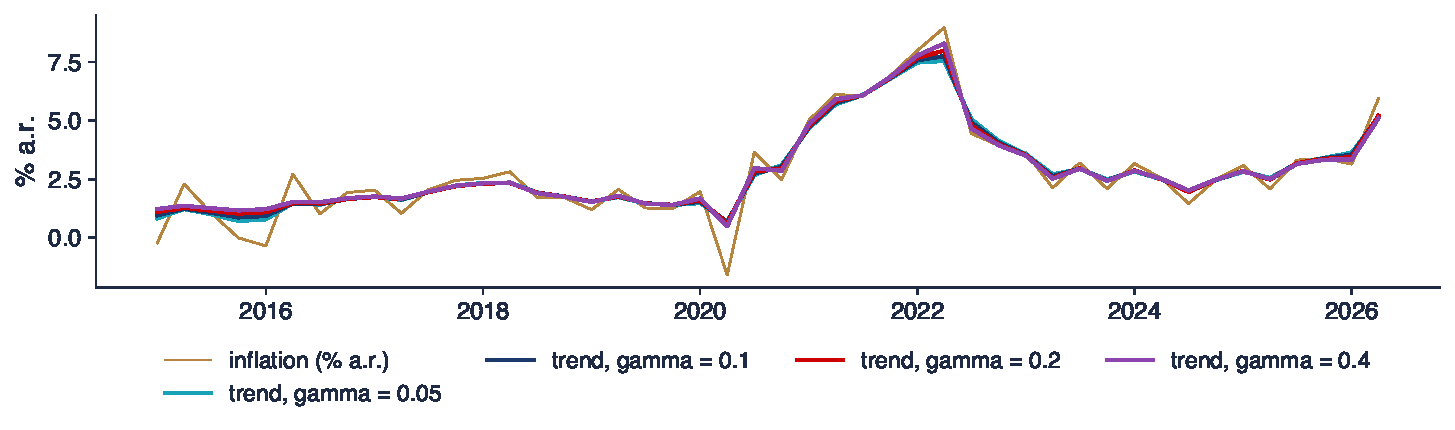
\includegraphics[width=0.97\textwidth,height=0.5\textheight,keepaspectratio]{ats_ch6_ai_case.pdf}
\end{center}
\vspace{-0.25cm}
\begin{itemize}
    \item US UC-SV trend since 2015 for $\gamma \in \{0.05, 0.1, 0.2, 0.4\}$: trend in 2022Q2 7.6, 7.8, 8.0, 8.3\% (inflation 9.0\%); in the last quarter 5.1, 5.2, 5.2, 5.1\%
    \item The ranking is stable but the level of the 2022 trend is not: an AI summary that reports ``trend inflation peaked at X\%'' without $\gamma$ hides a modelling choice
\end{itemize}
\quantlet{ATS\_ch6\_ai\_robustness}{\qlurl{ATS_ch6_ai_robustness}}
\end{frame}

\begin{frame}{Project idea}
\itemsize{\small}
\begin{itemize}
    \item \textbf{Trend inflation and anchoring in Central and Eastern Europe}: replicate first, then extend
    \begin{itemize}
        \item replicate: the US UC-SV trend of this lecture (2022Q2: 8.0\%) and the Romanian trend (7.3\% in 2026Q2)
        \item extend: Romania, Hungary, Poland and Czechia; a multivariate UC-SV with a common euro-area trend; administered prices as a separate component; $\gamma$ estimated with a prior instead of fixed
        \item pre-register: data, sample, priors, the anchoring statistic (posterior probability inside the target band), the real-time exercise and the robustness grid
    \end{itemize}
    \item Deliverables follow the course rules: repository, report, AI\_USE.md, AI\_ERRORS.md, oral defence
\end{itemize}
\end{frame}


%=============================================================================
\section{Wrap-up}
%=============================================================================

\begin{frame}{Key takeaways}
\itemsize{\small}
\begin{itemize}
    \item The Kalman filter is Gaussian conditioning applied recursively; the smoother, the likelihood and the simulation smoother follow from it
    \item Initialise nonstationary states exactly; treat zero variances as boundary problems
    \item Bayesian state space: sample whole paths; FFBS, DK and precision samplers are interchangeable
    \item Stochastic volatility is not GARCH; the KSC mixture and particle filters make it tractable
    \item Latent quantities (gaps, trends, time-varying slopes) come with model-dependent uncertainty: report bands, filtered values and alternatives
\end{itemize}
\end{frame}

\begin{frame}{Self-assessment}
\itemsize{\small}
\begin{columns}[T]
\begin{column}{0.58\textwidth}
\begin{block}{Questions}
\begin{itemize}
    \item Why does a big-kappa likelihood fall without bound as $\kappa$ grows?
    \item What does an ML estimate $\hat\sigma^2_\eta = 0$ tell you about a local level?
    \item Why does the DK simulation smoother need only a mean smoother?
    \item Why is the EKF gain zero in the SV model?
    \item Why is $\ln\hat L$ biased although $\hat L$ is unbiased?
    \item Which restriction makes the UC cycle differ from the BN cycle?
\end{itemize}
\end{block}
\end{column}
\begin{column}{0.38\textwidth}
\begin{block}{Next: \atschlink{https://danpele.github.io/Advanced-Time-Series/EN/Courses/chapter7_regime_switching_models.pdf}{Chapter 7}}
\begin{itemize}
    \item Regime-switching models
    \item Discrete hidden states: the Hamilton filter, the Kim smoother, EM and Gibbs for Markov switching, and state space models with regimes
\end{itemize}
\end{block}
\end{column}
\end{columns}
\end{frame}


%=============================================================================
\section{Appendix}
%=============================================================================

\begin{frame}{Appendix: the Kalman filter from the lemma}
\hypertarget{atsapp1}{}\atsappback{atssrc1}{Back}
\itemsize{\small}
\begin{itemize}
    \item Given $Y_{t-1}$: $\begin{pmatrix}\alpha_t\\ y_t\end{pmatrix} \sim N\left(\begin{pmatrix}a_t\\ Z_ta_t\end{pmatrix}, \begin{pmatrix}P_t & P_tZ_t'\\ Z_tP_t & F_t\end{pmatrix}\right)$, $F_t = Z_tP_tZ_t' + H_t$
    \item Conditioning on $y_t$ (equivalently on $v_t$, since $Y_t = (Y_{t-1}, v_t)$ and $v_t$ is independent of $Y_{t-1}$) gives $a_{t|t}$ and $P_{t|t}$
    \item $\alpha_{t+1} = c_t + T_t\alpha_t + R_t\eta_t$ with $\eta_t$ independent of $Y_t$: $a_{t+1} = c_t + T_ta_{t|t}$, $P_{t+1} = T_tP_{t|t}T_t' + R_tQ_tR_t'$
    \item Smoother: $\hat\alpha_t = a_t + \sum_{j=t}^n\Cov(\alpha_t, v_j)F_j^{-1}v_j$ (the $v_j$ are independent); $\Cov(\alpha_t, v_j) = P_tL_t'\cdots L_{j-1}'Z_j'$ gives $\hat\alpha_t = a_t + P_tr_{t-1}$
\end{itemize}
\end{frame}

\begin{frame}{Appendix: why the DK simulation smoother is exact}
\hypertarget{atsapp2}{}\atsappback{atssrc1}{Back}
\itemsize{\small}
\begin{itemize}
    \item Gaussian model: $\alpha | y \sim N(\hat\alpha(y), V)$ with $V$ independent of $y$, and $\hat\alpha(y)$ linear in $y$ (affine with the intercepts)
    \item For a draw $(\alpha^+, y^+)$ from the joint law, $\alpha^+ - \hat\alpha(y^+) \sim N(0, V)$ and is independent of $y^+$ (and of $y$)
    \item Hence $\tilde\alpha = \hat\alpha(y) + \alpha^+ - \hat\alpha(y^+) \sim N(\hat\alpha(y), V)$; linearity gives $\hat\alpha(y) - \hat\alpha(y^+) = \hat\alpha_0(y - y^+)$, one smoother pass with zero intercepts
    \item Diffuse states: the exact diffuse smoother is invariant to the diffuse part of $\alpha_1^+$, so it can be set to $a_1$
\end{itemize}
\end{frame}

\begin{frame}{Appendix: unbiasedness of the particle likelihood}
\hypertarget{atsapp3}{}\atsappback{atssrc1}{Back}
\itemsize{\small}
\begin{itemize}
    \item Bootstrap filter, one step: $\E[\frac1N\sum_iw^{(i)}_t\,|\,\mathcal F_{t-1}] = \int g(y_t | x)\,\hat p_{N}(x | Y_{t-1})\,dx$, with $\hat p_N$ the empirical predictive law of the particles
    \item Telescoping the conditional expectations over $t = n, n-1, \dots, 1$ with multinomial or systematic resampling gives $\E\prod_t\hat p(y_t | Y_{t-1}) = p(y_{1:n})$ \refDM
    \item Each factor is a ratio estimate, but the product is unbiased because resampling preserves the expected weights; normalised quantities (filtered means) are only consistent
    \item Jensen: $\E\ln\hat L \le \ln\E\hat L = \ln L$; under a CLT for $\ln\hat L$ the bias is $-\frac12\Var(\ln\hat L)$
\end{itemize}
\end{frame}


%=============================================================================
\section{References}
%=============================================================================

\begin{frame}{References (1/5)}
\itemsize{\tiny}
\begin{itemize}
    \item Aguiar, M., \& Gopinath, G. (2007). Emerging market business cycles: The cycle is the trend. \textit{Journal of Political Economy}, 115(1), 69--102. \href{https://doi.org/10.1086/511283}{doi:10.1086/511283}
    \item Andrieu, C., Doucet, A., \& Holenstein, R. (2010). Particle Markov chain Monte Carlo methods. \textit{Journal of the Royal Statistical Society: Series B}, 72(3), 269--342. \href{https://doi.org/10.1111/j.1467-9868.2009.00736.x}{doi:10.1111/j.1467-9868.2009.00736.x}
    \item Andrieu, C., \& Roberts, G. O. (2009). The pseudo-marginal approach for efficient Monte Carlo computations. \textit{The Annals of Statistics}, 37(2), 697--725. \href{https://doi.org/10.1214/07-AOS574}{doi:10.1214/07-AOS574}
    \item Ansley, C. F., \& Kohn, R. (1985). Estimation, filtering, and smoothing in state space models with incompletely specified initial conditions. \textit{The Annals of Statistics}, 13(4), 1286--1316. \href{https://doi.org/10.1214/aos/1176349739}{doi:10.1214/aos/1176349739}
    \item Bańbura, M., \& Modugno, M. (2014). Maximum likelihood estimation of factor models on datasets with arbitrary pattern of missing data. \textit{Journal of Applied Econometrics}, 29(1), 133--160. \href{https://doi.org/10.1002/jae.2306}{doi:10.1002/jae.2306}
    \item Beveridge, S., \& Nelson, C. R. (1981). A new approach to decomposition of economic time series into permanent and transitory components with particular attention to measurement of the `business cycle'. \textit{Journal of Monetary Economics}, 7(2), 151--174. \href{https://doi.org/10.1016/0304-3932(81)90040-4}{doi:10.1016/0304-3932(81)90040-4}
    \item Bollerslev, T. (1986). Generalized autoregressive conditional heteroskedasticity. \textit{Journal of Econometrics}, 31(3), 307--327. \href{https://doi.org/10.1016/0304-4076(86)90063-1}{doi:10.1016/0304-4076(86)90063-1}
    \item Brodersen, K. H., Gallusser, F., Koehler, J., Remy, N., \& Scott, S. L. (2015). Inferring causal impact using Bayesian structural time-series models. \textit{The Annals of Applied Statistics}, 9(1), 247--274. \href{https://doi.org/10.1214/14-AOAS788}{doi:10.1214/14-AOAS788}
    \item Carter, C. K., \& Kohn, R. (1994). On Gibbs sampling for state space models. \textit{Biometrika}, 81(3), 541--553. \href{https://doi.org/10.1093/biomet/81.3.541}{doi:10.1093/biomet/81.3.541}
    \item Chan, J. C. C., \& Jeliazkov, I. (2009). Efficient simulation and integrated likelihood estimation in state space models. \textit{International Journal of Mathematical Modelling and Numerical Optimisation}, 1(1/2), 101--120. \href{https://doi.org/10.1504/IJMMNO.2009.030090}{doi:10.1504/IJMMNO.2009.030090}
    \item Chopin, N., \& Papaspiliopoulos, O. (2020). \textit{An Introduction to Sequential Monte Carlo}. Springer. \href{https://doi.org/10.1007/978-3-030-47845-2}{doi:10.1007/978-3-030-47845-2}
    \item Clark, P. K. (1987). The cyclical component of U.S. economic activity. \textit{The Quarterly Journal of Economics}, 102(4), 797--814. \href{https://doi.org/10.2307/1884282}{doi:10.2307/1884282}
\end{itemize}
\end{frame}

\begin{frame}{References (2/5)}
\itemsize{\tiny}
\begin{itemize}
    \item Cogley, T., \& Sargent, T. J. (2001). Evolving post-World War II U.S. inflation dynamics. \textit{NBER Macroeconomics Annual}, 16, 331--373. \href{https://doi.org/10.1086/654451}{doi:10.1086/654451}
    \item Cogley, T., \& Sargent, T. J. (2005). Drifts and volatilities: Monetary policies and outcomes in the post WWII US. \textit{Review of Economic Dynamics}, 8(2), 262--302. \href{https://doi.org/10.1016/j.red.2004.10.009}{doi:10.1016/j.red.2004.10.009}
    \item de Jong, P. (1991). The diffuse Kalman filter. \textit{The Annals of Statistics}, 19(2), 1073--1083. \href{https://doi.org/10.1214/aos/1176348139}{doi:10.1214/aos/1176348139}
    \item de Jong, P., \& Shephard, N. (1995). The simulation smoother for time series models. \textit{Biometrika}, 82(2), 339--350. \href{https://doi.org/10.1093/biomet/82.2.339}{doi:10.1093/biomet/82.2.339}
    \item Del Moral, P. (2004). \textit{Feynman--Kac Formulae: Genealogical and Interacting Particle Systems with Applications}. Springer. \href{https://doi.org/10.1007/978-1-4684-9393-1}{doi:10.1007/978-1-4684-9393-1}
    \item Del Negro, M., \& Primiceri, G. E. (2015). Time varying structural vector autoregressions and monetary policy: A corrigendum. \textit{The Review of Economic Studies}, 82(4), 1342--1345. \href{https://doi.org/10.1093/restud/rdv024}{doi:10.1093/restud/rdv024}
    \item Doucet, A., Pitt, M. K., Deligiannidis, G., \& Kohn, R. (2015). Efficient implementation of Markov chain Monte Carlo when using an unbiased likelihood estimator. \textit{Biometrika}, 102(2), 295--313. \href{https://doi.org/10.1093/biomet/asu075}{doi:10.1093/biomet/asu075}
    \item Doz, C., Giannone, D., \& Reichlin, L. (2011). A two-step estimator for large approximate dynamic factor models based on Kalman filtering. \textit{Journal of Econometrics}, 164(1), 188--205. \href{https://doi.org/10.1016/j.jeconom.2011.02.012}{doi:10.1016/j.jeconom.2011.02.012}
    \item Durbin, J., \& Koopman, S. J. (2002). A simple and efficient simulation smoother for state space time series analysis. \textit{Biometrika}, 89(3), 603--616. \href{https://doi.org/10.1093/biomet/89.3.603}{doi:10.1093/biomet/89.3.603}
    \item Durbin, J., \& Koopman, S. J. (2012). \textit{Time Series Analysis by State Space Methods} (2nd ed.). Oxford University Press. \href{https://doi.org/10.1093/acprof:oso/9780199641178.001.0001}{doi:10.1093/acprof:oso/9780199641178.001.0001}
    \item Frühwirth-Schnatter, S. (1994). Data augmentation and dynamic linear models. \textit{Journal of Time Series Analysis}, 15(2), 183--202. \href{https://doi.org/10.1111/j.1467-9892.1994.tb00184.x}{doi:10.1111/j.1467-9892.1994.tb00184.x}
    \item Frühwirth-Schnatter, S., \& Wagner, H. (2010). Stochastic model specification search for Gaussian and partial non-Gaussian state space models. \textit{Journal of Econometrics}, 154(1), 85--100. \href{https://doi.org/10.1016/j.jeconom.2009.07.003}{doi:10.1016/j.jeconom.2009.07.003}
\end{itemize}
\end{frame}

\begin{frame}{References (3/5)}
\itemsize{\tiny}
\begin{itemize}
    \item Giannone, D., Reichlin, L., \& Small, D. (2008). Nowcasting: The real-time informational content of macroeconomic data. \textit{Journal of Monetary Economics}, 55(4), 665--676. \href{https://doi.org/10.1016/j.jmoneco.2008.05.010}{doi:10.1016/j.jmoneco.2008.05.010}
    \item Gordon, N. J., Salmond, D. J., \& Smith, A. F. M. (1993). Novel approach to nonlinear/non-Gaussian Bayesian state estimation. \textit{IEE Proceedings F (Radar and Signal Processing)}, 140(2), 107--113. \href{https://doi.org/10.1049/ip-f-2.1993.0015}{doi:10.1049/ip-f-2.1993.0015}
    \item Hamilton, J. D. (1994). \textit{Time Series Analysis}. Princeton University Press. \href{https://doi.org/10.2307/j.ctv14jx6sm}{doi:10.2307/j.ctv14jx6sm}
    \item Hamilton, J. D. (2018). Why you should never use the Hodrick--Prescott filter. \textit{The Review of Economics and Statistics}, 100(5), 831--843. \href{https://doi.org/10.1162/rest_a_00706}{doi:10.1162/rest\_a\_00706}
    \item Harvey, A. C. (1990). \textit{Forecasting, Structural Time Series Models and the Kalman Filter}. Cambridge University Press. \href{https://doi.org/10.1017/CBO9781107049994}{doi:10.1017/CBO9781107049994}
    \item Harvey, A. C., \& Jaeger, A. (1993). Detrending, stylized facts and the business cycle. \textit{Journal of Applied Econometrics}, 8(3), 231--247. \href{https://doi.org/10.1002/jae.3950080302}{doi:10.1002/jae.3950080302}
    \item Harvey, A., Ruiz, E., \& Shephard, N. (1994). Multivariate stochastic variance models. \textit{The Review of Economic Studies}, 61(2), 247--264. \href{https://doi.org/10.2307/2297980}{doi:10.2307/2297980}
    \item Jacquier, E., Polson, N. G., \& Rossi, P. E. (1994). Bayesian analysis of stochastic volatility models. \textit{Journal of Business \& Economic Statistics}, 12(4), 371--389. \href{https://doi.org/10.1080/07350015.1994.10524553}{doi:10.1080/07350015.1994.10524553}
    \item Julier, S. J., \& Uhlmann, J. K. (2004). Unscented filtering and nonlinear estimation. \textit{Proceedings of the IEEE}, 92(3), 401--422. \href{https://doi.org/10.1109/JPROC.2003.823141}{doi:10.1109/JPROC.2003.823141}
    \item Jungbacker, B., \& Koopman, S. J. (2015). Likelihood-based dynamic factor analysis for measurement and forecasting. \textit{The Econometrics Journal}, 18(2), C1--C21. \href{https://doi.org/10.1111/ectj.12029}{doi:10.1111/ectj.12029}
    \item Kalman, R. E. (1960). A new approach to linear filtering and prediction problems. \textit{Journal of Basic Engineering}, 82(1), 35--45. \href{https://doi.org/10.1115/1.3662552}{doi:10.1115/1.3662552}
    \item Kamber, G., Morley, J., \& Wong, B. (2018). Intuitive and reliable estimates of the output gap from a Beveridge--Nelson filter. \textit{The Review of Economics and Statistics}, 100(3), 550--566. \href{https://doi.org/10.1162/REST_a_00691}{doi:10.1162/REST\_a\_00691}
\end{itemize}
\end{frame}

\begin{frame}{References (4/5)}
\itemsize{\tiny}
\begin{itemize}
    \item Kim, C.-J., \& Nelson, C. R. (1999). \textit{State-Space Models with Regime Switching: Classical and Gibbs-Sampling Approaches with Applications}. MIT Press. \href{https://doi.org/10.7551/mitpress/6444.001.0001}{doi:10.7551/mitpress/6444.001.0001}
    \item Kim, S., Shephard, N., \& Chib, S. (1998). Stochastic volatility: Likelihood inference and comparison with ARCH models. \textit{The Review of Economic Studies}, 65(3), 361--393. \href{https://doi.org/10.1111/1467-937X.00050}{doi:10.1111/1467-937X.00050}
    \item Kitagawa, G. (1996). Monte Carlo filter and smoother for non-Gaussian nonlinear state space models. \textit{Journal of Computational and Graphical Statistics}, 5(1), 1--25. \href{https://doi.org/10.1080/10618600.1996.10474692}{doi:10.1080/10618600.1996.10474692}
    \item Koopman, S. J. (1997). Exact initial Kalman filtering and smoothing for nonstationary time series models. \textit{Journal of the American Statistical Association}, 92(440), 1630--1638. \href{https://doi.org/10.1080/01621459.1997.10473685}{doi:10.1080/01621459.1997.10473685}
    \item Koopman, S. J., \& Durbin, J. (2000). Fast filtering and smoothing for multivariate state space models. \textit{Journal of Time Series Analysis}, 21(3), 281--296. \href{https://doi.org/10.1111/1467-9892.00186}{doi:10.1111/1467-9892.00186}
    \item Mariano, R. S., \& Murasawa, Y. (2003). A new coincident index of business cycles based on monthly and quarterly series. \textit{Journal of Applied Econometrics}, 18(4), 427--443. \href{https://doi.org/10.1002/jae.695}{doi:10.1002/jae.695}
    \item Morley, J. C., Nelson, C. R., \& Zivot, E. (2003). Why are the Beveridge--Nelson and unobserved-components decompositions of GDP so different? \textit{The Review of Economics and Statistics}, 85(2), 235--243. \href{https://doi.org/10.1162/003465303765299765}{doi:10.1162/003465303765299765}
    \item Omori, Y., Chib, S., Shephard, N., \& Nakajima, J. (2007). Stochastic volatility with leverage: Fast and efficient likelihood inference. \textit{Journal of Econometrics}, 140(2), 425--449. \href{https://doi.org/10.1016/j.jeconom.2006.07.008}{doi:10.1016/j.jeconom.2006.07.008}
    \item Orphanides, A., \& van Norden, S. (2002). The unreliability of output-gap estimates in real time. \textit{The Review of Economics and Statistics}, 84(4), 569--583. \href{https://doi.org/10.1162/003465302760556422}{doi:10.1162/003465302760556422}
    \item Petropoulos, F., Apiletti, D., Assimakopoulos, V., Babai, M. Z., et al.\ (2022). Forecasting: Theory and practice. \textit{International Journal of Forecasting}, 38(3), 705--871. \href{https://doi.org/10.1016/j.ijforecast.2021.11.001}{doi:10.1016/j.ijforecast.2021.11.001}
    \item Pitt, M. K., \& Shephard, N. (1999). Filtering via simulation: Auxiliary particle filters. \textit{Journal of the American Statistical Association}, 94(446), 590--599. \href{https://doi.org/10.1080/01621459.1999.10474153}{doi:10.1080/01621459.1999.10474153}
    \item Pitt, M. K., Silva, R. d. S., Giordani, P., \& Kohn, R. (2012). On some properties of Markov chain Monte Carlo simulation methods based on the particle filter. \textit{Journal of Econometrics}, 171(2), 134--151. \href{https://doi.org/10.1016/j.jeconom.2012.06.004}{doi:10.1016/j.jeconom.2012.06.004}
\end{itemize}
\end{frame}

\begin{frame}{References (5/5)}
\itemsize{\tiny}
\begin{itemize}
    \item Primiceri, G. E. (2005). Time varying structural vector autoregressions and monetary policy. \textit{The Review of Economic Studies}, 72(3), 821--852. \href{https://doi.org/10.1111/j.1467-937X.2005.00353.x}{doi:10.1111/j.1467-937X.2005.00353.x}
    \item Scott, S. L., \& Varian, H. R. (2014). Predicting the present with Bayesian structural time series. \textit{International Journal of Mathematical Modelling and Numerical Optimisation}, 5(1/2), 4--23. \href{https://doi.org/10.1504/IJMMNO.2014.059942}{doi:10.1504/IJMMNO.2014.059942}
    \item Shephard, N., \& Harvey, A. C. (1990). On the probability of estimating a deterministic component in the local level model. \textit{Journal of Time Series Analysis}, 11(4), 339--347. \href{https://doi.org/10.1111/j.1467-9892.1990.tb00062.x}{doi:10.1111/j.1467-9892.1990.tb00062.x}
    \item Shumway, R. H., \& Stoffer, D. S. (1982). An approach to time series smoothing and forecasting using the EM algorithm. \textit{Journal of Time Series Analysis}, 3(4), 253--264. \href{https://doi.org/10.1111/j.1467-9892.1982.tb00349.x}{doi:10.1111/j.1467-9892.1982.tb00349.x}
    \item Stock, J. H., \& Watson, M. W. (1998). Median unbiased estimation of coefficient variance in a time-varying parameter model. \textit{Journal of the American Statistical Association}, 93(441), 349--358. \href{https://doi.org/10.1080/01621459.1998.10474116}{doi:10.1080/01621459.1998.10474116}
    \item Stock, J. H., \& Watson, M. W. (2007). Why has U.S. inflation become harder to forecast? \textit{Journal of Money, Credit and Banking}, 39(s1), 3--33. \href{https://doi.org/10.1111/j.1538-4616.2007.00014.x}{doi:10.1111/j.1538-4616.2007.00014.x}
    \item Taylor, S. J. (1994). Modeling stochastic volatility: A review and comparative study. \textit{Mathematical Finance}, 4(2), 183--204. \href{https://doi.org/10.1111/j.1467-9965.1994.tb00057.x}{doi:10.1111/j.1467-9965.1994.tb00057.x}
    \item Watson, M. W. (1986). Univariate detrending methods with stochastic trends. \textit{Journal of Monetary Economics}, 18(1), 49--75. \href{https://doi.org/10.1016/0304-3932(86)90054-1}{doi:10.1016/0304-3932(86)90054-1}
\end{itemize}
\end{frame}

\end{document}
